%%%%%%%%%%%%%%%%%%%%%%%%%%%%%%%%%%%%%%%%%%%%%%%%%%%%
%
% compile the document with
% latex, bibtex, makeindex, latex, latex
%
%%%%%%%%%%%%%%%%%%%%%%%%%%%%%%%%%%%%%%%%%%%%%%%%%%%%
\documentclass{style/icon_docu_style}
\newcommand{\versnr}{1.8.00}
\newcommand{\doctitle}{ICON User's Guide }

% ------------------------------------------------------
% define a base path for TeX-includes
% ------------------------------------------------------
\newcommand*{\basepath}{../}%


% ------------------------------------------------------
% define new commands here
% ------------------------------------------------------
\newcommand{\icon}{ICON}
\newcommand{\echam}{ECHAM}


\begin{document}

% Title
% This is a list of authors of the ICON User Guide and ICON Technical Documentation sorted by their affiliation.

%-------
% KIT
%-------

\newcommand{\riegerd}{D. Rieger}
\newcommand{\vogelb}{B. Vogel}
\newcommand{\krauti}{I. Kraut}
\newcommand{\vogelh}{H. Vogel}
\newcommand{\schadt}{T. Schad}
\newcommand{\walterc}{C. Walter}
\newcommand{\grubers}{S. Gruber}
\newcommand{\deetzk}{K. Deetz}

%-------
% DWD
%-------

\newcommand{\zaenglg}{G. Z\"angl}
\newcommand{\reinertd}{D. Reinert}
\newcommand{\prillf}{F. Prill}
\newcommand{\frankh}{H. Frank}
\newcommand{\heinzet}{T. Heinze}
\newcommand{\majewskid}{D. Majewski}
\newcommand{\rhodina}{A. Rhodin}
\newcommand{\ritterb}{B. Ritter}
\newcommand{\ripodasp}{P. R\'\i{}podas}
\newcommand{\baldaufm}{M. Baldauf}
\newcommand{\domsg}{G. Doms}
\newcommand{\foerstnerj}{J. F\"orstner}
\newcommand{\heisee}{E. Heise}
\newcommand{\herzogh}{H.-J. Herzog}
\newcommand{\mironovd}{D. Mironov}
\newcommand{\raschendorferm}{M. Raschendorfer}
\newcommand{\reinhardtt}{T. Reinhardt}
\newcommand{\schrodinr}{R. Schrodin}
\newcommand{\schulzj}{J.-P. Schulz}
\newcommand{\vogelg}{G. Vogel}


%-------
% MPI
%-------

\newcommand{\ronnebergerk}{K. Ronneberger}
\newcommand{\linardakisl}{L. Linardakis}
\newcommand{\bonaventural}{L. Bonaventura}
\newcommand{\eschm}{M. Esch}
\newcommand{\giorgettam}{M. Giorgetta}
\newcommand{\kornp}{P. Korn}
\newcommand{\kornbluehl}{L. Kornblueh}
\newcommand{\schulzweidau}{U. Schulzweida}
\newcommand{\muellerr}{R. M\"uller}
\newcommand{\lorenzs}{S. Lorenz}
\newcommand{\dipankara}{A. Dipankar}
\newcommand{\wanh}{H. Wan}
\newcommand{\gassmanna}{A. Gassmann}
\newcommand{\rasts}{S. Rast}
\newcommand{\muellers}{S. M\"uller}
\newcommand{\ram}{R. M\"uller}

\renewcommand\Affilfont{\itshape\normalsize}

\titlehead{  
\unitlength = 1mm  
\begin{picture}(80,0)  
\put(-10,-10){ 
\includegraphics[scale=0.3]{../pictures/mpilogo.pdf} }  
\put(63,-20){\makebox(0,0)[rb]{\textbf{Max-Planck-Institut f\"ur Meteorologie}}}
\put(63,-24){\makebox(0,0)[rb]{Bundesstr. 53}}
\put(63,-29){\makebox(0,0)[rb]{D-20146 Hamburg}}
\end{picture}
\hspace{1cm}
\begin{picture}(80,0)
\put(13.9,-10){ 
\includegraphics[scale=0.2]{../pictures/dwdlogo.png} }  
\put(72,-20){\makebox(0,0)[rb]{\textbf{Deutscher Wetterdienst}}}
\put(72,-24){\makebox(0,0)[rb]{Frankfurter Str. 135}}
\put(72,-29){\makebox(0,0)[rb]{D-63067 Offenbach}}
\end{picture} 
\begin{picture}(80,0)  
\put(58,-150){ 
\includegraphics[scale=0.08]{../pictures/kitlogo.jpg} }  
\put(78,-160){\makebox(0,0)[cb]{\textbf{Karlsruhe Institute of Technology}}}
\put(78,-165){\makebox(0,0)[cb]{Institute for Meteorology and Climate Research (IMK-TRO)}}
\put(78,-169){\makebox(0,0)[cb]{Hermann-von-Helmholtz-Platz 1}}
\put(78,-174){\makebox(0,0)[cb]{D-76344 Eggenstein-Leopoldshafen}}
\end{picture} 
\begin{picture}(80,0)  
\put(0,-125){\makebox(0,0)[cb]{\textbf{assembled and edited by}}}
\put(0,-130){\makebox(0,0)[cb]{\textbf{\schadt, \krauti, \riegerd, \walterc, \grubers, \deetzk, \vogelh, and \vogelb}}}
\end{picture} 
} 


\title{\vspace{6cm}ICON User's Guide}  

\author{\hspace{2cm}\zaenglg}
\author{\reinertd}
\author{\prillf}
\author{\newline\giorgettam}
\author{\kornbluehl}
\author{\linardakisl}


\affil{}%Karlsruhe Institute of Technology (KIT)\\
%Institute for Meteorology and Climate Research (IMK-TRO)}  
%\affil[2]{Deutscher Wetterdienst\\Frankfurter Str. 135\\D-63067 Offenbach\\Germany}  
%\affil[3]{Max-Planck-Institut f\"ur Meteorologie\\Bundesstr. 53\\D-20146 Hamburg\\Germany}   


\date{\vspace{8cm}\today}  

\maketitle

\begin{abstract}

\section*{Preface}



This user guide was assembled and edited based on available documents on the 
ICON webpage by the persons mentioned at the front page. The content of the user guide follows the requirements of DWD.


\textit{Important hints:}

In chapter 4 a list of the namelist parameters is given. New and inexperienced users should only modify the namelist parameters that are given in bold letters. 




When results produced with ICON are published the following papers have to be cited
in the list of references:

\cite{Zaengl:2013}


\end{abstract}

\newpage
\par\vspace*{\fill}
\begin{center}\textbf{Information for authors:}

\textbf{Please read the README for further instructions and tamplates.}
\end{center}
\pagenumbering{roman}
\pagestyle{fancyplain}
\renewcommand{\footrulewidth}{0.4pt}
\renewcommand{\plainheadrulewidth}{0.4pt}
\renewcommand{\plainfootrulewidth}{0.4pt}

\lhead[\bf\thepage]{\small\sffamily Contents}
\rhead[\small\sffamily Contents]{\bf\thepage}
\lfoot[\footnotesize\sffamily Contents]%
      {\footnotesize\sffamily \doctitle -- \versnr}
\rfoot[\footnotesize\sffamily \doctitle -- \versnr]%
      {\footnotesize\sffamily Contents}
\cfoot{}

%Contents page
\ifpdf
\hypertarget{IX}{\tableofcontents}
\else
\tableofcontents
\fi
\clearpage


\ifpdf
\rhead[\small\sffamily\rightmark]{\hyperlink{IX}{\bf\thepage}}
\lhead[\hyperlink{IX}{\bf\thepage}]{\small\sffamily\rightmark}
\else
\rhead[\small\sffamily\rightmark]{\bf\thepage}
\lhead[\bf\thepage]{\small\sffamily\rightmark}
\fi
\lfoot[\footnotesize\sffamily\leftmark]%
      {\footnotesize\sffamily \doctitle -- \versnr}
\rfoot[\footnotesize\sffamily \doctitle -- \versnr]%
      {\footnotesize\sffamily\leftmark}

\pagenumbering{arabic}
\setcounter{page}{1}


% Place new content here
\chapter{Guide for New Users}

\newcommand{\netcdf}{NetCDF}

%%%%%%%%%%%%%%%%%%%%%%%%%%%%%%%%%%%%%%%%%%%%%%%
% Progression Bar
% |==============>   |
% empty chapter        chapter finished
%%%%%%%%%%%%%%%%%%%%%%%%%%%%%%%%%%%%%%%%%%%%%%%

This tutorial is meant for people with some knowledge and/or experience in modelling and Linux, but which have no experience with the ICON model. In the following we will describe in short how to compile and run ICON on your machine. 

\section{Needed Software}

For some components ICON uses external libraries. Therefore you will need some additional software which should be installed on your machine. The following software needed to be installed on your machine:

\begin{itemize}
 \item \netcdf : \netcdf is a set of software libraries and self-describing, machine-independent data formats that support the creation, access, and sharing of array-oriented scientific data.\newline
 (Source: \href{http://www.unidata.ucar.edu/software/netcdf/}{http://www.unidata.ucar.edu/software/netcdf/})
 \item GRIB: GRIB (GRIdded Binary) is a format defined by the WMO (World Meteorological Organization). The use of GRIB in ICON is optional. The ECMWF GRIB API is an application program interface accessible from C, FORTRAN and Python programs developed for encoding and decoding WMO FM-92 GRIB edition 1 and edition 2 messages. A useful set of command line tools is also provided to give quick access to GRIB messages. \newline
 (Source: \href{https://software.ecmwf.int/wiki/display/GRIB/Home}{https://software.ecmwf.int/wiki/display/GRIB/Home})
 \item MPI: MPI is a library specification for message-passing, proposed as a standard by a broadly based committee of vendors, implementors, and users.\newline
 (Source: \href{http://www.mcs.anl.gov/research/projects/mpi/}{http://www.mcs.anl.gov/research/projects/mpi/})
 \item OpenMP: Jointly defined by a group of major computer hardware and software vendors, the OpenMP API is a portable, scalable model that gives shared-memory parallel programmers a simple and flexible interface for developing parallel applications on platforms ranging from embedded systems and accelerator devices to multicore systems and shared-memory systems.\newline
 (Source: \href{http://openmp.org/wp/}{http://openmp.org/wp/})
\end{itemize}

\section{The Source Code}
% Filenames and URL needs to be adapted
You can obtain the source code on the website of DKRZ:

\href{https://www.dkrz.de/}{https://www.dkrz.de/}

You can use the following commands to untar the ICON source code:

\begin{verbatim}
tar xfvz icon.tar.gz
\end{verbatim}

This will create a folder \verb+icon-1.0+ inside your current directory. Within the ICON User Guide, this folder will further on be called \verb+$ICONDIR+.

\subsection{Directory structure}

Within \verb+$ICONDIR+, you will find a set of subdirectories. The important subdirectories are described in the following. 

\subsubsection{build}

Within the \verb+$ICONDIR/build+ directory, a subdirectory with the name of your computer architecture is created at compilation. Within this subdirectory, a \verb+bin+ subdirectory containing the binary \verb+control_model+ and several further subdirectories containing the compiled module files are created at compilation. 

\subsubsection{config}

Inside the \verb+$ICONDIR/config+ directory, different machine dependent configuration are stored within the configuration files. You can find a description of how to use and set up such configuration files in chapter \ref{chap:UG_config_compil}.

\subsubsection{data}

Within the \verb+$ICONDIR/data+ directory, you will find divers input datasets. For example, there are the datasets \verb+"rrtmg_lw.nc"+ and \verb+"ECHAM6_CldOptProps.nc"+, which are necessary for the radiation scheme (see sec. \ref{InputReal:Rad}). 

\subsubsection{doc}

Within the \verb+$ICONDIR/doc+ directory, several documentations for ICON are stored. There are according subdirectories for scientific (\verb+$ICONDIR/doc/science+), technical (\verb+$ICONDIR/doc/technical+) and programming style guides (\verb+$ICONDIR/doc/style+).

\subsubsection{externals}

Within the \verb+$ICONDIR/externals+ directory, external libraries for ICON are stored. Currently, it is the mtime library which is used to convert different date time formats.

\subsubsection{include}

Within the \verb+$ICONDIR/include+ directory, interfaces to libraries needed by ICON are stored. Currently, the interface to the CDI library is stored inside this directory. 

\subsubsection{run}

Within the \verb+$ICONDIR/run+ directory, namelist descriptor files as well as the full namelist documentation are stored. The namelist descriptor files can be used to generate runscripts. Further information can be found in \ref{chap:UG_running_model}.

\subsubsection{src}

Within the \verb+$ICONDIR/src+ directory, the source code of ICON including the main program and ICON modules can be found. The modules are ordered in several subdirectories which are described in the following. 

The main program \verb+control_model.f90+ can be found inside the subdirectory \newline \verb+$ICONDIR/src/drivers+. Additionally, this directory contains the modules for a hydrostatic and a nonhydrostatic setup.

The configuration of an ICON run is performed within the modules inside \newline \verb+$ICONDIR/src/configure_model+ and \verb+$ICONDIR/src/namelists+. Modules regarding the configuration of idealized test cases can be found inside \verb+$ICONDIR/src/testcases+.

The dynamics of ICON are inside \verb+$ICONDIR/src/atm_dyn_iconam+ and the physical parameterizations inside \verb+$ICONDIR/src/atm_phy_nwp+. Parameterizations for the interactions with the surface can be found inside \verb+$ICONDIR/src/lnd_phy_nwp+.

Shared infrastructure modules for 3-D and 4-D variables can be found within \newline \verb+$ICONDIR/src/shared+. The according routines for 2-D fields (e.g. external parameters) are stored within \verb+$ICONDIR/src/shr_horizontal+.

Modules handling the parallelization can be found in \newline\verb+$ICONDIR/src/parallel_infrastructure+.

Input and output modules are stored in \verb+$ICONDIR/src/io+.

The modules for the grid generator, as described in chapter \ref{chap:UG_grid_generation} can be found inside \newline \verb+$ICONDIR/src/grid_generator+.

\subsubsection{vertical\_coord\_table}

Inside the \verb+$ICONDIR/vertical_coord_tables+ directory, information files describing the relation between model layer, pressure and height are stored.

\section{Configuration and Compilation}
\label{chap:UG_config_compil}

%Configure and Compile

To ease up the compilation a configure-file is provided which should take over the main work. This Autoconf configuration is used to analyze the computer architecture (hardware and software) and set user specified preferences, e.g. the compiler. This preferences are read from \verb+config/mh-<OS>+, where \verb+<OS>+ is the identified operating system. Operating systems are listed in the configure-files in \verb+$ICONDIR/config/+ with the according files \verb+mh-<OS>+. If your machine is not listed you can add a config-file with your own \verb+<OS>+ based on the given \verb+mh-<OS>+ files. If different compilers are available, the \verb+mh-<OS>+ file may contain a case construct to distinguish them. If your \verb+<OS>+ is not recognized but is one of the listed \verb+<OS>+ you can invoke the configure file with the according option \verb+--host=$HOST+. Examples for the DWD CRAY system are given in the boxes.

\subsection{Description of the Configuration Files}

To add a specific compiler or change your compiler flags, you have to enter the \newline \verb+$ICONDIR/config/mh-<OS>+ according to your operating system \verb+<OS>+. For the DWD CRAY, the compiler flags in \verb+mh-linux+ look like the following:

\begin{Verbatim}[frame=single]
cray)
    config_compiler=cray
	CC          = cc
    FC          = ftn
    F77         = "$FC"
    FFLAGS      = -v -D__LOOP_EXCHANGE -D__MIXED_PRECISION -Df2cFortran 
-e Z -em -hflex_mp=conservative -hfp1 -hadd_paren -r am -Ktrap=divz,ovf
    CFLAGS      = -I${GRIB_API}/include -v -Df2cFortran 
-DHAVE_CF_INTERFACE -DHAVE_LIBNETCDF -DHAVE_LIBGRIB 
-DHAVE_LIBGRIB_API -O3  -D__SVN_VERSION="${SVNVERSION}"
    F77FLAGS    = "$FFLAGS"
    FCLIBS      = "-v"
    GEN_FLAGS   =
    FDEBUG      = -g -R abc
    OMPFLAG     = -mp
    DEFOPT      = -D
    DEFCOPT     = -D
    MODOPT      = -I
    MODDIR      = 
    ;;
\end{Verbatim}

The \verb+cray)+ in this example gives the name of this specific configuration. It can be addressed by a flag at configuration. For this example, the according command to choose this setting would be \verb+./configure --with-fortran=cray+ (see section \ref{sec:config_compile}). Like this, you can create your own configuration by adding a new compiler.

\verb+CC+, \verb+FC+ and \verb+F77+ are the compiler directives for C-Compiler, FORTRAN2003-Compiler and FORTRAN77-Compiler. The according compiler flags are set via \verb+CFLAGS+, \verb+FFLAGS+ and \verb+F77FLAGS+. The variable to set an OpenMP flag is called \verb+OMPFLAG+. Libraries are set via \verb+FCLIBS+. 

\subsection{Configuring and Compiling the Code} \label{sec:config_compile}

To configure the source code go to \verb+$ICONDIR+ and give:

\begin{small}
 \begin{verbatim}
  ./configure
  ./build_command
  \end{verbatim}
\end{small}

If you want to use another compiler than the default compiler you give:

\begin{small}
  \begin{verbatim}
   ./configure --with-fortran=<compiler>
   ./build_command
  \end{verbatim}
\end{small}

where \verb+<compiler>+ is \verb+{gcc,nag,intel,pgi,cray}+.

\begin{Verbatim}[frame=single]
CRAY EXAMPLE: Configure + Make
./configure --with-fortran=cray}
./build_command
\end{Verbatim}

Note, that CRAY compiler environment (cce) versions 8.2.x do not work with ICON. The CRAY configuration is expanded to the following:

\begin{Verbatim}[frame=single]
CRAY EXAMPLE: Configuration
ftn -I../module -v -D__LOOP_EXCHANGE -D__MIXED_PRECISION -Df2cFortran -e 
Z -em -hflex_mp=conservative -hfp1 -hadd_paren -r am -Ktrap=divz,ovf 
-D__ICON__ <object files> -L/usr/local/pkg/grib_api/1.11.0/CRAY/lib  
-L../lib -lsupport -lgrib_api_f90 -lgrib_api -lmtime $(LAPACK_LIB) 
$(NETCDF_LIB) $(HDF5_LIB) $(SZIP_LIB) $(ZLIB_LIB) $(MPI_LIB) 
$(METIS_LIB) $(PROFILE_LIB) $(SCT_LIB)
\end{Verbatim}

ICON is parallelized using MPI and OpenMP. You can control the parallelization to be used by giving:

\begin{small}
  \begin{verbatim}
   ./configure --with-mpi/--without-mpi --with-openmp/--without-openmp
   ./build_command
  \end{verbatim}
\end{small}

By default the options are set to \verb+--with-mpi --without-openmp+. After a successful build, you will find the ICON executable named \verb+control_model+ inside \verb+$ICONDIR/build/<OS>/bin/+.

\begin{Verbatim}[frame=single]
CRAY EXAMPLE: OpenMP
The CRAY Fortran compiler command includes automatically OpenMP. 
Therefore, although using --without-openmp, OpenMP is used.
\end{Verbatim}

If you wish to re-configure ICON it is advisable first to clean the old setup by giving:

\begin{small}
  \begin{verbatim}
   make distclean  
  \end{verbatim}
\end{small}

Some more details on configure options can be found in the help of the configure command:

\begin{small}
 \begin{verbatim}
  ./configure --help
 \end{verbatim}
\end{small}

\section{Running the Model (Idealized Cases)}
\label{chap:UG_running_model_idealized}

To shed light on the functionality and the quality of the dynamical core, setups for two test cases are presented in the following. Additionally, results of these test cases are shown. These tests are classified in short deterministic test cases (typically a simulation period of about 10-30 days) and tests in a climate mode (typically a multi-year period). This section concentrates on the first class, which starts from prescribed initial conditions (ideally provided in analytic form). The simulation results are either compared to analytic solutions (if available) or high-resolution reference solutions. %% http://www-personal.umich.edu/~cjablono/dycore_test_suite.html (access: 07.02.2014, last updated: 2012)
For testcase details the reader is referred to \cite{Zaengl:2013}. Here only some special setups are described.

\subsection{Jablonowski-Williamson test}

The Jablonowski-Williamson Test \citep{Jablonowski:2006} is a standard test for dynamical cores in global models and can be run for dry dynamics only - as it is intended for- but full physics can be also tested. 

\subsubsection{Setup}

For full physics, two additional namelist parameters are introduced in the  \verb+testcase_nml+ to control the initial moisture in the atmosphere:
\begin{itemize}
\item Here \verb+rh_at_1000hpa+ to be set between $0$ and $1$. The default is set to $0.7$ which gives a quite smooth start. If you really want to see early onsets of convection and microphysics you have to tune this parameter.
\item \verb+qv_max+ is usually set to $20.e-3 kg/kg$ and refers to the maximum value in the tropics.
\end{itemize}

\subsubsection{Input Data}

GRID

\subsubsection{Results}

The \textbf{Jablonowski-Williamson steady-state test} is based on a zonally symmetric, strongly baroclinic atmosphere. Initially, it is in a hydrostatic and geostrophic balance and therefore should remain stationary if no perturbation is imposed. Grid irregularities can disturb this stationary conditions and hence the test identifies the presence and magnitude of grid imprinting of a numerical model.
For the \textbf{Jablonowski-Williamson baroclinic wave test}, a weak (and unbalanced) perturbation disturbs the initial wind. This test highlights the diffusivity (or effective resolution) of a dynamical core and the presence of phase speed errors in the advection of poorly resolved structures.

\subsection{Mountain Rossby wave}

In order to test the model dynamics in dry stage but with real or any complex topography one can choose the mountain rossby wave test and select different types of topography.

\subsubsection{Setup}

 By setting this, you might want to have the turbulence scheme switched on while the rest of physics is switched OFF. Simulating dry physics means to set the tracer fields to zero. The transport is not necessary but should be switched off via the transport namelist, so the resulting namelist setting for this case is:
\begin{itemize}
\item \verb+testcase_nml+
 \begin{itemize}
  \item  \verb+nh_test_name  = 'mrw_nh'+
 \end{itemize}
\end{itemize}
As an extreme case the user can examine the flow over very steep mountains, by using a flow of an isothermal atmosphere with 
$U = 20  \rm \, m \, s^{-1}$ over a circular Gaussian mountain
\begin{align}
h(x,y) = h_m \exp \left( - \frac{x^2 + y^2}{a^2} \right)
\end{align}
with $a = 2000\,\mathrm{m}$ and $h_m = 4000\,\mathrm{m}$ and $7000\,\mathrm{m}$, respectively. 
This configuration produces slope angles of 59$^\circ$ and 71$^\circ$. However, \cite{Zaengl:2013} recommend  to avoid slope angles close to or even above 70$^\circ$ in scientific applications.

\subsubsection{Input Data}

GRID

\subsubsection{Results}



\section{Running the Model (Real Case)}
\label{chap:UG_running_model}


The ICON code, as checkout from the SVN repository, does not include runscripts. Instead the run directory (\verb+$ICONDIR/run/+) includes several descriptor files for building grids, defining experiments and post-processings. There exist three different types of descriptor files with prefixes \verb+grid, exp, post+:

\begin{itemize}
 \item \verb+grid.<name>+: to configure the grid generator, see chapter \ref{chap:UG_grid_generation} for more details. It is recommended to use pre-built grids. For details, see section \ref{chap:prebuilt_grid}.
 \item \verb+exp.<name>+: to define the namelist, which determinate the experiments.
 \item \verb+post.<name>+: to define post-processing.
\end{itemize}

\subsection{Input Data}

Generally ICON requires the following input data: Grid files, external parameters, initialization (DWD analysis or IFS), input fields for radiation.

\subsubsection{Grid Files}\label{sec:grid_input}

In order to run ICON, it is necessary to have the horizontal grid information as an input parameter. This information is stored within so-called grid files. For a ICON run, one global grid file is necessary. Additionally, if you want to nest, grid files of the nested domains are necessary, too. To improve the performance of ICON, a (optional) reduced radiation grid for each domain may be used. 

The naming of the ICON-Grid is as follows: The initial icosahedron grid is refined by \textless n\textgreater -secting the edges, and further refinement is obtained by iteratively bisecting the created edges. The grid produced at the \textless k\textgreater refining iteration is named "R\textless n\textgreater B\textless k\textgreater". For further details, see the ICON Technical Documentation.

It is recommended to use pre-built grids. Further information can be found in chapter \ref{chap:prebuilt_grid}. For building own grids, the reader is referred to chapter \ref{chap:UG_grid_generation}. The names of the grid files have to be specified within the \verb+grid_nml+:

\begin{verbatim}
&grid_nml
dynamics_grid_filename = "<INSERTFILENAME>"
radiation_grid_filename = "<INSERTFILENAME>"
\end{verbatim}

\subsubsection{External Parameters}\label{InputReal:Ext}

ICON requires geographical localized datasets like the topographic height of the earth surface, the plant cover, the distribution of land and sea and, dependent on the schemes used, a variety of other so called external parameters. The EXTPAR software system (EXTPAR - External Parameter for Numerical Weather Prediction and Climate Application) is able to generate external parameters for the different models GME, COSMO, HRM and ICON. The software can run on a UNIX or Linux systems where the raw data is stored. It allows operators (experienced users) running the scripts to create new external parameters controlled by user specifications like the model domain. For a more detailed overview of EXTPAR, the reader is referred to the User and Implementation Guide of EXTPAR. 

The name of the EXTPAR file which has to be read by ICON can be specified as follows:

\begin{verbatim}
&extpar_nml
extpar_filename = "<INSERTFILENAME>"
\end{verbatim}

If not specified explicitly, ICON uses the following file name: \newline
\verb+"<path>extpar_<gridfile>"+.\newline
 \verb+<path>+ and \verb+<gridfile>+ are then replaced at runtime by ICON.

\subsubsection{Initialization}\label{InputReal:Ini}

For the initialization of ICON, input data from either DWD or IFS is needed. 

In case of DWD (init\_mode=1) a first guess and an analysis is required: 
\begin{verbatim}
&initicon_nml
dwdfg_filename = "<INSERTFILENAME>"
dwdana_filename = "<INSERTFILENAME>"
\end{verbatim}

If not specified explicitly, ICON uses the following file names: \newline 
\verb+"<path>dwdFG_R<n>B<k>_DOM<idom>.nc"+ and \newline
\verb+"<path>dwdana_R<n>B<k>_DOM<idom>.nc"+. \newline
\verb+<path>+, \verb+<n>+, \verb+<k>+ and \verb+<idom>+ are then replaced at runtime by ICON according to the chosen gridfile (see \ref{sec:grid_input}). The variable \verb+<idom>+ is an index for the domain on which the calculations are performed. \verb+<idom>=0000+ is reserved for a reduced radiation grid, \verb+<idom>=0001+ for the global domain, higher numbers are used for nested domains. NETCDF as well as GRIB2 input can be used.

In case of IFS (init\_mode=2) an analysis is required. It has to be in \netcdf: 
\begin{verbatim}
&initicon_nml
ifs2icon_filename = "<INSERTFILENAME>"
\end{verbatim}

If not specified explicitly, ICON uses the following file name: \newline 
\verb+"<path>ifs2icon_R<n>B<k>_DOM<idom>.nc"+. \newline
\verb+<path>+, \verb+<n>+, \verb+<k>+ and \verb+<idom>+ are then replaced at runtime by ICON according to the chosen gridfile (see \ref{sec:grid_input}). The variable \verb+<idom>+ is an index for the domain on which the calculations are performed. \verb+<idom>=0000+ is reserved for a reduced radiation grid, \verb+<idom>=0001+ for the global domain, higher numbers are used for nested domains.

\subsubsection{Radiation}\label{InputReal:Rad}

ICON requires input fields for the RRTM radiation scheme. The file names are specified as follows:

\begin{verbatim}
&nwp_phy_nml
lrtm_filename = "<INSERTFILENAME>" 
cldopt_filename = "<INSERTFILENAME>"
\end{verbatim}

If not specified explicitly, ICON uses the following file names: \newline 
\verb+"rrtmg_lw.nc"+ and \newline
\verb+"ECHAM6_CldOptProps.nc"+.

The files can be found within \verb+$ICONDIR/data+.

\subsection{Creating a Runscript}

To create a runscript, new users are advised to use the namelist descriptor file \verb+exp.nh-oper+ which contains recently recommended namelist settings. It might be necessary to account for the file names and paths of the input data. Additionally, machine dependent settings need to be added to this script to obtain a runscript. For some architectures, this step can be performed by using the make runscript environment as shown in \ref{sec:make_runscript}. In the following, example settings for DWD CRAY are listed.

\begin{Verbatim}[frame=single]
CRAY EXAMPLE: Environment variables
#!/bin/ksh
#==============================================================
#PBS -q xc_normal
#PBS -l select=?:ncpus=?:mpiprocs=?:ompthreads=?:mem=?gb
#PBS -l place=scatter
#PBS -j oe
#PBS -N <<Jobname>>

export MPICH_RMA_OVER_DMAPP=1
\end{Verbatim}

\begin{Verbatim}[frame=single]
CRAY EXAMPLE: Namelists
<<Place your namelists e.g. from exp.nh_oper here>>
\end{Verbatim}

\begin{Verbatim}[frame=single]
CRAY EXAMPLE: Submitting a job
aprun                                    \
  -n <<INSERT: MPI Tasks>>            \
  -N <<INSERT: MPI Tasks/Node>>       \
  <<INSERT: Hyperthreading e.g. 2 -> 20 physical -> 40 "virtual" cores>> \
  -d <<INSERT: Threads/MPI Task>>     \
  -m <<INSERT: Amount of memory to use>> control_model
\end{Verbatim}


\subsection{Restart}

A restart of the model requires a restart file that has to be created by a 
previous model run. In the following the procedures and the corresponding namelist settings are explained.

\subsubsection{Creating the initial restart file:}

The first job in a series of model runs creates the first restart file.
To do so we have to use the following namelist switches.

\begin{verbatim}
&master_nml
lrestart = .FALSE. 
\end{verbatim}

In addition we have to prescribe at which time interval the job should produce a restart file:

\begin{verbatim}
&io_nml
dt_checkpoint = "<Insert time in seconds>" 
\end{verbatim}


The ICON run then creates restart files for each domain 1, ..., \verb+n_dom+, and for each restart
output time step. 

The filenames are generic and look like:

\begin{verbatim}
 "<gridfile>_restart_<modeltype>_<timestamp>.nc", 
\end{verbatim}

An example would be:

\begin{verbatim}
 "iconR2B06_DOM01_restart_atm_20110101T001200Z.nc"    (NetCDF format)
\end{verbatim}
   
This filename can be customized using the namelist parameter:
    
     
\begin{verbatim}
&mo_run_nml
restart_filename = "<INSERTFILENAME>" 
\end{verbatim}

This file contains:

\begin{itemize}
\item{data} 
\item{namelists}
\item{several attributes}
\end{itemize}


Note:
    -  ICON reads the namelists only once and assumes that these
       are identical for all domains.
    -  Since we do not know about the total number of domains at startup,
       we have to ask the current restart file for the attribute \verb+"n_dom"+.


For each domain 1, ..., \verb+n_dom+, a symbolic link is generated with the generic name: 

 \verb+"restart_<modeltype>_DOMxx.nc"+

     
     
 
Note:
    -  The domain-dependent suffix "...DOMxx" is also required for 
non-nested setups.

    


\subsubsection{Running the model in the restart mode:}

ICON has to be informed that you want to carry out a restart run:

\begin{verbatim}
&master_nml
lrestart = .TRUE. 
\end{verbatim}

The generic link \verb+"restart_<modeltype>_DOMxx.nc"+ is used by the restart run to point to the last written restart file of the previous model run. 


\subsubsection*{Chain of restart runs}

If a chain of restart runs is foreseen it is recommended to use the namelist parameter
\verb+dt_restart+. 

\begin{verbatim}
&time_nml
dt_restart = "<Insert time in seconds>" 
\end{verbatim}


In this case only one restart file is produced by each model run and after writing the restart file the job stops.

Note:- \verb+dt_restart+ and \verb+dt_checkpoint+ have to be selected carefully. 
 


\subsubsection*{Asynchronous in- and  output:} 

It is highly recommended that the asynchronous in- and output option of ICON is applied. In short this option reserves a number of processors for in- and output only.  While reading and writing the remaining processors continuously carry out calculations. Otherwise they would have to wait until in- or output is finished. The corresponding namelist parameter is:

\begin{verbatim}
&parallel_nml
num_restart_procs = n
\end{verbatim} 

n is the number of processors used for in- and output. 

Note: n=1 is the most efficient selection.


\subsection{Make Runscript Environment}\label{sec:make_runscript}


A full listing of descriptor files you will find in \verb+$ICON/run/+. 

After configuration and compiling (chapter \ref{chap:UG_config_compil}) these descriptor files can be transformed into runscripts, which should include the necessary system dependent parameters and the execution section \verb+exec.icon+ (\verb+$ICONDIR/run/exec.iconrun+), which starts the actual integration. This transformation is done in \verb+$ICONDIR+ by:

\begin{small}
 \begin{verbatim}
  ./make_runscripts
 \end{verbatim}
\end{small}

This transforms every existing descriptor file in \verb+$ICONDIR/run/<type>.<name>+ into a ready-to-use run script \verb+$ICONDIR/run/<type>.<name>.run+

For illustration there exists also 

\begin{small}
 \begin{verbatim}
  ./make_my_runscripts
 \end{verbatim}
\end{small}

which transforms a single descriptor file into a run script. This file is an exemplary file and you can see how to define run parameters.

An exemplary descriptor file for a operational run is \verb+exp.nh_oper+.

\textbf{Note:} if you change, or create a descriptor you will need to (re)create the run script in order for the changes to take effect.

To run a script \verb+<type>.<name>.run+, either for creating grids or making an experiment or doing post-processing, go to the \verb+./run+ folder

\begin{small}
  \begin{verbatim}
   cd run
  \end{verbatim}
\end{small}

and use the job submission command, which depends on your machine:

\begin{small}
  \begin{verbatim}
   [<submit>] <type>.<name>.run
  \end{verbatim}
\end{small} 

\verb+[<submit>]+ is something like: \verb+{llsubmit,qsub}+

\textbf{Note:} \underline{Before} (!) running an experiment, the ICON grids must be available to the model. For this purpose, either pre-built grids and ExtPar Data can be used (see Sec. \ref{chap:prebuilt_grid}) or create own grids (\ref{chap:UG_grid_generation}). For a new user, it is suggested to use pre-built grids first.

\section{Pre-built Grids and ExtPar Data}\label{chap:prebuilt_grid}
A list of grid files has been pre-built for the ICON model together with the corresponding reduced radiation grids and the external parameters.

\begin{enumerate}
\item The \textbf{primary storage} location for ICON grids is
\begin{small}
 \begin{verbatim}
  blizzard:/pool/data/ICON/grids/public 
 \end{verbatim}
\end{small}
\item Every 24h the contents of the primary storage directory are mirrored to DWD's HPC.
\item Every 24h the contents of the primary storage directory are mirrored to a public web site:
\href{http://icon-downloads.zmaw.de}{http://icon-downloads.zmaw.de}.
\end{enumerate}

Each grid file consists of a NetCDF file and a GPG signature file\\ 
(\href{http://de.wikipedia.org/wiki/GNU\_Privacy\_Guard}{http://de.wikipedia.org/wiki/GNU\_Privacy\_Guard}).\\ 
The signature file makes sure that a grid file is complete and verifies the authorship.

\subsection{Grid file nomenclature}
The grids are identified by
\begin{itemize}
\item a \textbf{centre} number
\item a \textbf{subcentre} number
\item a \textbf{numberOfGridUsed}\\
which is simply an integer number, increased by one with every new \lq official\rq\ grid.  
\end{itemize}

The grid files and the external parameter files are named accordingly, e.g.,
\begin{small}
 \begin{verbatim}
  icon_grid_0001_RxxByy_G.nc
  icon_extpar_0001_RxxByy_G.nc 
 \end{verbatim}
\end{small}
where the name components are as follows:
\begin{small}
 \begin{verbatim}
 icon _	grid   _ 0001 _	R 02 B 06 _	R                   .nc 
                                     (radiation/reduced)
 icon _ extpar _ 0002 _	  03   07 _	G                   .nc
                                     (global)         
                 ...      ...  ...
 \end{verbatim}
\end{small}

The \verb+numberOfGridUsed+ parameter is part of the file name (0001, ...) and makes this file name unique.

In general, a lookup table is required to find the actual file name to which a set of these parameters corresponds. 
This \lq table file\rq\ is located under 
\begin{center}
  {\tt http://icon-downloads.zmaw.de/dwd\_grids.xml} 
\end{center}
(the table file itself is under version control: \href{https://svn.zmaw.de/svn/icon\_grid\_table}{https://svn.zmaw.de/svn/icon\_grid\_table}). 



%\subsection{How does the XML grid description look like?}
%The table is stored in XML format, which is more or less human-readable. It consists of paragraphs of the following form:
%
%\begin{small}
% \begin{verbatim}
%    <grid  oper                = "yes"
%           number_of_grid_used = "2"
%           centre              = "78"
%           subcentre           = "255"
%           type                = "horizontal">
%     <description>
%           Global R02B06 grid.
%           40 km resolution
%     </description>
%     <uri>grids/public/edzw/icon_grid_0002_R02B06_G.nc</uri>
%     <extpar>
%      <uri>grids/public/edzw/icon_extpar_0002_R02B06_G.nc</uri>
%      <description>Globcover-based data set.</description>
%     </extpar>
%    </grid>
% \end{verbatim}
%\end{small}
%
%\begin{itemize}
%\item The optional oper attribute allows to mark a specific grid as operational. 
%\item The \verb+<description>+ tag allows to describe the grid properties in a few words. 
%\end{itemize}
%
%The XML file can also be \textbf{viewed in a web browser}
%\begin{small}
% \begin{verbatim}
%  firefox --no-remote ${ICON_XML_GRID_TABLE}
% \end{verbatim}
%\end{small}
%
%where the table layout is then defined by the XSL definitions in \verb+xml/dwd_grids.xsl+. 
%\begin{itemize}
%\item The XML file will later be available in tabular form on the public grid web site. 
%\end{itemize}
%
%Finally, the XML file contains information on \textbf{associated grids} (e.g., refinement hierarchies):
%\begin{small}
% \begin{verbatim}
%    <gridset>
%      <description>
%        Global R02B04 grid hierarchy without nests.
%      </description>
%      <grid number_of_grid_used = "9"  
%            centre              = "78"
%            subcentre           = "255"
%            type                = "horizontal" />
%      <grid number_of_grid_used = "10"  
%            centre              = "78"
%            subcentre           = "255"
%            type                = "horizontal" />
%    </gridset>
% \end{verbatim}
%\end{small}

\section{Grid Generation}
\label{chap:UG_grid_generation}
\subsection{ICON atmosphere grids}

The ICON horizontal spherical grid is based on the projection of the icosahedron on the sphere. This is a 2-dimensional grid, representing the earth's surface. For defining the vertical discretization see the Experiments section. The ICON grids need to be created, stored as \netcdf~ files, and consequently used by the ICON model. Alternatively, already stored grids maybe used.

The initial icosahedron grid is refined by \textless n\textgreater -secting the edges, and further refinement is obtained by iteratively bisecting the created edges. The grid produced at the \textless k\textgreater refining iteration is named "R\textless n\textgreater B\textless k\textgreater", and the corresponding \netcdf -file is \verb+"iconR<n>B<k>-grid.nc"+. The grid files, after their creation, are located in the ./grids folder.

Examples of grids are in Grids. More information can be found in\\ 
\verb+$ICONDIR/doc/technical/icon_grid.pdf+

\subsection{Creating atmosphere grids}

The descriptor file for creating the atmosphere grids is \verb+./run/grid.create_atmo_grids+. It generates 5 levels of icon grids using spring dynamics and symmetry optimizations. In addition it creates an hierarchy of three nested grids for the \verb+exp.nat_jww_nwp_mpiomp+ experiment (source: \verb+$ICONDIR/run/exp.nat_jww_nwp_mpiomp+).

For creating the run script \verb+$ICONDIR/run/grid.create_atmo_grids.run+, give

\begin{small}
  \begin{verbatim}
   ./make_runscripts
  \end{verbatim}
\end{small}

To submit it, go to \verb+$ICONDIR/run+ and give

\begin{small}
  \begin{verbatim}
   [<submit>] grid.create_atmo_grids.run 
  \end{verbatim}
\end{small}

See chapter \ref{chap:UG_running_model} how to generate run scripts for more information on creating and running scripts.

After running the \verb+grid.create_atmo_grids.run+, the \netcdf -grid-files will be located in the \verb+$ICONDIR/grids+ folder.

\textbf{Note} that the grid generator is only OpenMP parallelized and not MPI parallelized.


%\subsection{Creating ocean grids}
%
%The descriptor file for creating the ocean grids is \verb+$ICONDIR/run/grid.create_ocean_grids+. It generates four ocean grids for specific experiments. These are enabled through the parameters in the beginning of the descriptor:
%\begin{small}
%  \begin{verbatim}
%   \#-----------------------------------------------------------------------------
%   create_basin=".true." 
%   create_aqua_planet=".true." 
%   create_etopo40_flat=".true." 
%   create_etopo40_planet=".true." 
%   \#-----------------------------------------------------------------------------
%  \end{verbatim}
%\end{small}
%
%
%The ocean grids are created based on topography (etopo40), geometric constrains (basin), or aqua planet (aqua\_planet). You should not modify this descriptor unless you are familiar with the details of the ocean grid generation.
%After running the \verb+grid.create_ocean_grids.run+, which is the same procedure as shown for atmosphere grids, the \netcdf~ grid files will be located in the \verb+$ICONDIR/grids/+ folder.


\subsection{Atmosphere grid generation parameters}

In the beginning of the descriptor file \verb+$ICONDIR/run/grid.create_atmo_grids+ the basic atmosphere grid generation parameters are defined:

\begin{small}
  \begin{verbatim}
#-----------------------------------------------------------------------------
# if make_patches="true", the hierarchy of nested patches
#   iconR2B03_DOM00.nc, iconR2B04_DOM01.nc, iconR2B05_DOM02.nc
#   will be created
make_patches="true" 

# define number of levels (bisections) to create
no_of_levels=5

#define optimization
use_spring_optimization="true"          
use_symmetry_optimization="true" 
start_optimize=2
end_optimize=$no_of_levels

# define refinement method
refinement_method=1     # 1=edge bisection, 2=dual centers
#-----------------------------------------------------------------------------
  \end{verbatim}
\end{small}


The script variable \verb+no_of_levels+ defines the number of bisecting iterations (after the initial bisection), and determines the horizontal resolution. It is set to \verb+no_of_level=5+, giving in the highest resolution the triangular grid R2B05 of 81920 triangles, with a mean distance of 70\,km between triangle circumcenters, where scalars are defined. You may increase the resolution by increasing the \verb+no_of_levels+.

%\subsection{Ocean grid generation parameters}
%
%In the script \verb+$ICONDIR/run/grid.create_ocean_grids+ the basic ocean grid generation parameters are defined.
%
%There are 4 methods within this script to create an ocean grid file, which can be switched on/off independently:
%
%\begin{small}
%  \begin{verbatim}
%\#-----------------------------------------------------------------------------
%create_aqua_planet=".true." 
%create_etopo40_flat=".true." 
%create_etopo40_planet=".true." 
%create_basin=".true." 
%\#-----------------------------------------------------------------------------
%  \end{verbatim}
%\end{small}
%
%\begin{itemize}
% \item[] Aqua planet (no land) for ocean alone or coupled model integrations
% \item[] Create a land-sea-mask and a flat bottom bathymetry (depth \$SEADEPTH)
% \item[] Create a land-sea-mask including an ocean bathymetry interpolated from the ETOPO bathymetry with 40 minutes resolution min\_sea\_depth=\$LSMDEPTH gives the value to decide whether a point is land or sea
% \item[] Create special geometric conditions (basins, channels)
%\end{itemize}
%
%For example a bathymetry for a circumpolar channel with flat bottom uses the following parameters:
%
%\begin{small}
%  \begin{verbatim}
% # grid parameters
%  R=2                   # nroot: bisectional refinement
%  B=4                   # no. of bisections applied for the global grid
%  REFINE_ITERATIONS=3   # no. of refinements after smoothing ocean boundary
%                        #  - resolution for smoothing is ((B-REFINE_ITERATIONS)) 
%                        # optimize_ocean_grids=".true." 
%
%  #bathymetry parameters
%  SEADEPTH="-12000.0"   # set ocean bathymetry to constant (flat bottom)
%  INTMTH=3              # edge elevation interpolation method: 1= linear, 2=min,  3=max
%  # topography file
%  TOPFILE=""            # no topography file used for the basin
%  #conditions
%  no_of_conditions=1    # use parameter for new Stommel basin (see below)
%  patch_shape=1         # 1=orthogonal, 2= circle 
%  rectangle_xradious=180.0   # circumpolar (360 deg)
%  rectangle_yradious=15.0    #  30 deg meridional extent
%
%  # output grid name
%  OCEGRID=iconR\$RB0\${B}-ocean_chan-45N.nc   #  zonal circumpolar channel
%  \end{verbatim}
%\end{small}
%
%Generated grids are located at the \verb+$ICONDIR/grids/+ directory
	
\subsection{Information contained in grid files}

The ICON grids are treated as a general unstructured grid, so the grid \netcdf -files contain the full information of the location and the connectivity of all the grid entities (cells, edges and vertices). The grid nesting hierarchy information is also included.

Some basic variables that may be useful for plotting are:

\begin{small}
  \begin{verbatim}
double clon(cell)                : longitude of cell centers [radian]
double clat(cell)                : latitude  of cell centers [radian]
double clon_vertices(cell, nv)   : longitudes of the vertices of the cell [radian]
double clat_vertices(cell, nv)   : latitudess of the vertices of the cell [radian]
double elon(edge)                : longitude of edge midpoint [radian]
double elat(edge)                : latitude  of edge midpoint [radian]
double elon_vertices(edge, no)   : longitudes of the vertices of the edges [radian]
double elat_vertices(edge, no)   : latitudes  of the vertices of the edges [radian]
double vlon(vertex)              : longitude of vertices [radian]
double vlat(vertex)              : latitude  of vertices [radian]
...
double cell_area(cell)           : area of grid cell [m2]
double cell_elevation(cell)      : elevation at the cell centers [m]
int    cell_sea_land_mask(cell): sea (-2 inner, -1 boundary) 
                                   land (2 inner, 1 boundary) mask for the cell
...
double edge_length(edge)         : lengths of edges of triangular cells [m]
double dual_edge_length(edge)   : lengths of dual edges (distances between
                                   triangular cell circumcenters) [m]
...
  \end{verbatim}
\end{small}

For a full listing of variables contained in a grid file, for instance in iconR2B04-grid.nc, use:

\begin{small}
  \begin{verbatim}
   ncdump -h iconR2B04-grid.nc  
  \end{verbatim}
\end{small}

or

\begin{small}
  \begin{verbatim}
   cdo sinfov iconR2B04-grid.nc
  \end{verbatim}
\end{small}


More details on the grid fields can be found \href{https://code.zmaw.de/projects/icon/repository/entry/trunk/icon-1.3.00/doc/technical/icon\_grid.pdf} {\tt here}.\\

\subsection{Viewing/plotting grids}

In order to plot an icon grid you should ensure that \verb+ncl-6.0+ and \verb+cdo-1.5.4+ is available on your machine. Then go to the \verb+$ICONDIR/grids/+ folder and give:

\begin{small}
  \begin{verbatim}
alias iplot="ncl $ICONDIR/scripts/postprocessing/tools/icon_plot.ncl 
'altLibDir="$ICONDIR/scripts/postprocessing/tools/"'" iplot 'iFile="<grid file name>"' 
'mapType="ortho"' 'varName="cell_sea_land_mask"' 'oType="png"' 'showGrid=True' 
'lStrg="Cell sea land mask"' 'bStrg=""'
  \end{verbatim}
\end{small}



The above example will plot cell sea land mask. More details on plotting can be found at the Visualization chapter.

The \verb+$ICONDIR/run/post.plot_icon_grids+ script can be used to plot nested grids. Go to \verb+$ICONDIR/run/+ folder and give:

\begin{small}
  \begin{verbatim}
   ./post.plot_icon_grids  
  \end{verbatim}
\end{small}

A PDF-file with a plot of the iconR2B04\_DOM01 and iconR2B05\_DOM02 grids will appear on your screen. (Note that this process is time consuming.)

\newpage
\subsection*{Discussion}
%This section is for discussion only. Please add your notes, your name and date.
Document last edited by \textit{S Gruber} on \textit{08-01-2014}
Document last edited by \textit{B Vogel} on \textit{27-05-2014}.

\chapter{Output}

%%%%%%%%%%%%%%%%%%%%%%%%%%%%%%%%%%%%%%%%%%%%%%%
% Progression Bar
% |==> |
% empty chapter chapter finished
%%%%%%%%%%%%%%%%%%%%%%%%%%%%%%%%%%%%%%%%%%%%%%%


In general the user has to specify six individual quantities to generate output of the model. These are:

\begin{enumerate}
\item{The time interval between two model outputs.}
\item{The name of the output file.}
\item{The name of the variable.}
\item{The type of the vertical output grid (e.g. pressure levels or model levels).}
\item{The type of the horizontal output grid (e.g. ICON grid or geographical coordinates).}
\end{enumerate}

ICON offers the possibility to write groups of variables. 
In the following we will present two examples to demonstrate the options the user has to prescribe these quantities. A detailed description of all namelist parameters available to organize the output is described  in \verb+io_nml+ in the namelist section.

\subsubsection{Example 1}

We will begin with an individual variable which is written in NETCDF format on pressure levels and is interpolated to a horizontally regular lat-long grid:

\begin{Verbatim}[frame=single]
NAMELIST EXAMPLE
&io_nml
 filetype                  =  4   ! output format: 2=GRIB2, 4=NETCDFv2
 dom                       =  1   ! write output for domain 1
 output_bounds             =  0., 1.E7, 3600. ! start, end, interval in s.
 steps_per_file            =  50  ! max. num. of time steps within one file
 mode                      =  1   ! 1: forecast mode (relative t-axis)
 include_last              = .TRUE. ! include the last time step
 output_filename           = '<INSERTFILENAME>' ! file name base
 pl_varlist                = 'geopot' ! name of pressure level field
 remap                     = 1   ! output is transferred to lat long grid
 reg_lon_def               = 0.,0.5,359.5   !start, incr., end, in deg.
 reg_lat_def               = 90.,-0.5, -90. !start, incr., end, in deg.
\end{Verbatim}




\subsubsection{Example 2}

The flexibility of the options ICON offers is demonstrated in another example. Now we apply an alternative to define the runtime of ICON, write several variables, at the same time, in one data set, on model levels, and on the original horizontal grid of ICON. In addition the example below shows the options when several model domains run at the same time and we want to produce output for all model domains.

\begin{Verbatim}[frame=single]
NAMELIST EXAMPLE
&output_nml
 dom                          =  -1 ! write all domains
 steps_per_file               =  5  ! max. num. of time steps within
  output_start     = "1978-01-01T00:00:00Z" ! ISO-format date+time
  output_end       = "1979-01-02T00:00:00Z" ! ISO-format date+time
  output_interval  = "PT01H"                ! ISO-format interval
  file_interval    = "PT01D"                ! ISO-format interval
  include_last     = .FALSE.
  output_filename              = '<INSERTFILENAME>'    ! file name base
  ml_varlist='u', 'group:precip_vars' ! Indiv. variable and variable group
  output_grid      = .TRUE. ! Output on the ICON horizontal grid
\end{Verbatim}

\subsubsection{Variable groups}
Next we explain the meaning of variable groups.
Using the \texttt{"group:"} keyword for the namelist parameters \texttt{ml\_varlist}, \texttt{hl\_varlist}, \texttt{pl\_varlist},
sets of common variables can be added to the output.


There exists a special syntax which allows to remove variables from the output list, e.\,g.\ if
these undesired variables were contained in a previously selected group.\\
Typing \texttt{"-<varname>"} (for example \texttt{"-temp"}) removes the
variable from the union set of group variables and other selected variables.Note that typos are not detected but that the corresponding variable is simply not removed!



\subsubsection{How to find variable names and contents of variable groups}

Finding the correct names of the variables you may want to write to a data set is not an easy task and you should be aware of some pitfalls. We will help you to avoid the most obvious ones. First of all users that have already experience with the COSMO model should know that the names of the atmospheric variables in ICON are \textbf{not identical}. 

The easiest way to identify the correct names of the variables you would like to write is to look into the following data sets:

\begin{Verbatim}[frame=single]
atm_dyn_iconam/mo_nonhydro_state.f90
atm_phy_nwp/mo_nwp_phy_state.f90
lnd_phy_nwp/mo_nwp_lnd_state.f90
\end{Verbatim}

Now you may want to use the option of writing groups of variables and of course you may want to know which variable belongs to which group.
Keep in mind that there is an option mentioned before to remove variables from the output of a group of variables.

The following table gives overview on the allocation of variables to individual variable groups. If you want to translate the Fortran variables to the physical or mathematical ones again have a look to the Fortran files listed above.

\begin{Verbatim}[frame=single]
******************************
	nh_prog_vars
vn
rho
theta_v
exner
******************************
	dwd_fg_atm_vars
vn
w
rho
theta_v
tke
u
v
pres_sfc
temp
pres
z_ifc
t_2m
td_2m
u_10m
v_10m
******************************
	mode_dwd_fg_in
vn
w
rho
theta_v
tke
t_g
t_mnw_lk
t_wml_lk
h_ml_lk
t_bot_lk
c_t_lk
t_b1_lk
h_b1_lk
qv_s
w_i
w_so_ice
w_snow
rho_snow
t_snow_mult
rho_snow_mult
wliq_snow
wtot_snow
dzh_snow
gz0
******************************
	atmo_ml_vars
w
tke
u
v
temp
pres
******************************
	atmo_pl_vars
w
tke
u
v
temp
******************************
	atmo_z1_vars
w
tke
u
v
temp
pres
******************************
	mode_dwd_ana_in
u
v
temp
pres
t_ice
h_ice
fr_seaice
w_so
t_snow
h_snow
freshsnow
******************************
	atmo_derived_vars
omega
div
vor
******************************
	land_vars
t_g
qv_s
w_i
w_p
w_s
t_so
w_so
w_so_ice
t_snow
w_snow
rho_snow
snowfrac
******************************
	dwd_fg_sfc_vars
t_g
t_ice
h_ice
fr_seaice
w_i
t_so
w_so
w_so_ice
t_snow
w_snow
rho_snow
h_snow
freshsnow
t_snow_mult
rho_snow_mult
wliq_snow
wtot_snow
dzh_snow
gz0
******************************
	mode_combined_in
t_g
t_ice
h_ice
qv_s
fr_seaice
w_i
w_so
t_snow
w_snow
rho_snow
h_snow
freshsnow
******************************
	mode_cosmode_in
t_g
t_ice
h_ice
qv_s
w_i
w_so
t_snow
w_snow
rho_snow
h_snow
freshsnow
******************************
	dwd_fg_scf_vars	
t_mnw_lk 
t_wml_lk  
h_ml_lk  
t_bot_lk  
c_t_lk 
t_b1_lk  
h_b1_lk 
qv_s
******************************
	land_tile_vars
t_g_t
t_s_t
w_i_t
w_p_t
w_s_t
t_so_t
w_so_t
w_so_ice_t
t_snow_t
w_snow_t
rho_snow_t
t_snow_mult_t
wtot_snow_t
wliq_snow_t
rho_snow_mult_t
dzh_snow_t
qv_s_t
h_snow_t
snowfrac_t
snowfrac_lc_t
******************************
	snow_vars
t_snow
rho_snow
wliq_snow
wtot_snow
dzh_snow
******************************
	multisnow_vars
t_snow_mult
rho_snow_mult
wliq_snow
wtot_snow
dzh_snow
******************************
	precip_vars

rain_gsp
snow_gsp
rain_con
snow_con
ice_gsp
graupel_gsp
hail_gsp
tot_prec
******************************
	additional_precip_vars
con_prec_rate_avg 
gsp_prec_rate_avg
cape
clct
tot_cld_vi
******************************
	pbl_vars
gust
shfl_s
lhfl_s
lhfl_bs
lhfl_pl
ghfl_s
tcm
tch
t_2m 
qv_2m
td_2m  
u_10m  
v_10m 
tkvm
tkvh
******************************
	cloud_diag
clc
gc_dia
gi_dia
tot_cld
******************************
	rad_vars
thb_s
sod_t
sou_t
sod_s
sou_s
thd_s
thu_s
sodird_s
sodifd_s
sodufu_s
albdif
albvisdiff
albnirdiff
sob_s_t
thb_s_t
flxdwswtoa
sob_s
sob_t
******************************
	phys_tendencies
ddt_temp_radsw
ddt_temp_radlw
ddt_temp_turb
ddt_temp_drag
ddt_u_turb
ddt_u_sso
ddt_u_gwd
ddt_v_turb
ddt_v_sso
ddt_v_gwd: 
******************************
	prog_timemean
temp_m
rho_m
u_m
v_m
pres_sfc_m
pres_msl_m
******************************
	echam_timemean
cosmu0_m
flxdwswtoa_m
aclcov_m
rsfl_m
rsfc_m
ssfl_m
ssfc_m
totprec_m
qvi_m
xlvi_m
xivi_m
swflxsfc_m
swflxtoa_m
lwflxsfc_m
lwflxtoa_m
tsfc_m
evap_m
lhflx_m
shflx_m
u_stress_m
v_stress_m
******************************
	tracer_timemean
qc_m
qv_m
qi_m
******************************
	atmo_timemean
all vars of prog_timemean, echam_timmean, tracer_timemean
\end{Verbatim}

 

\subsubsection{Data format}


ICON offers the possibility to produce output either in NETCDF or GRIB2 format. This can be chosen by the namelist parameter \verb+filetype+ of the namelist \verb+&output_nml+. New users are suggested to set \verb+filetype=4+ in order to use NETCDF output.

In GRIB2, a variable is uniquely defined by the following set of metadata:
\begin{itemize}
 \item \textit{Discipline} (see GRIB2 code table 4.2)
 \item \textit{ParameterCategory} (see GRIB2 code table 4.2)
 \item \textit{ParameterNumber} (see GRIB2 code table 4.2)
 \item \textit{typeOfFirstfixedSurface} and \textit{typeOfSecondFixedSurface} (see GRIB2 code table 4.5)
 \item \textit{stepType} (instant, accum, avg, max, min, diff, rms, sd, cov, \dots)
\end{itemize}
A documentation of the official WMO GRIB2 code tables can be found on the website of WMO: \\ \href{http://www.wmo.int/pages/prog/www/WMOCodes/WMO306_vI2/LatestVERSION/WMO306_vI2_GRIB2_CodeFlag_en.pdf} {http://www.wmo.int/pages/prog/www/WMOCodes/ \\ WMO306\_vI2/LatestVERSION/WMO306\_vI2\_GRIB2\_CodeFlag\_en.pdf}.\\



\subsubsection{Time stamp format}


The namelist parameters \texttt{output\_start}, \texttt{output\_end}, \texttt{output\_interval} allow
the specification of time stamps according to ISO 8601.
The general format for time stamps is \texttt{YYYY-MM-DDThh:mm:ss}
where \texttt{Y}: year, \texttt{M}: month, \texttt{D}: day for dates, 
and   \texttt{hh}: hour, \texttt{mm}: minute, \texttt{ss}: second for time strings.  
The general format for durations is \texttt{PnYnMnDTnHnMnS}.
See, for example, \texttt{http://en.wikipedia.org/wiki/ISO\_8601} for details and further specifications.

\color{red}NOTE: as the mtime library underlaying the output driver
  currently has some restrictions concerning the specification of durations:\begin{enumerate}
\item Any number \texttt{n} in \texttt{PnYnMnDTnHnMnS} must have two digits. For instance use \texttt{"PT06H"} instead of \texttt{"PT6H"}
\item In a duration string \texttt{PnyearYnmonMndayDTnhrHnminMnsecS} the numbers \texttt{nxyz} must not pass the carry over number to the next larger time unit: 0$<$=nmon$<$=12, 0$<$=nhr$<$=23, 0$<$=nmin$<$=59, 0$<$=nsec$<$=59.999. For instance use \texttt{"PT01D"} instead of \texttt{"PT24H"}, or \texttt{"PT01M"} instead of \texttt{"PT60S"}.
\end{enumerate}

Soon the formatting problem will be resolved and the valid number ranges will be enlarged.
(2013-12-16).\color{black}



\subsubsection{Extra output}


\begin{enumerate} 
\item In the namelist {\bf \texttt{run\_ctl}} set the number of fields with \texttt{inextra\_2d} or
  \texttt{inextra\_3d}. The logical variable for output
  \texttt{lwrite\_extra} then will be set automatically. Note, the
  number of extra fields is limited by $9$ each for 2D and 3D.
\item  \texttt{USE} these variables in the module needed.
\item Implement the storage of wished fields by using the
  nonhydrostatic diagnostic type with
  \texttt{p\_diag\%extra\_2d/3d}. 
\end{enumerate} 

Example for the use of  \texttt{p\_diag\%extra\_2d}:  

\begin{small}
\begin{verbatim}
  USE mo_global_variables, ONLY: inextra_2d
...
  DO jc = i_startidx, i_endidx
p_diag\%extra_2d(jc,jb,1)= yxz(jc,jb)
  ENDDO
\end{verbatim}
\end{small}


\subsubsection*{Asynchronous output:}
It is highly recommended that the asynchronous output option of ICON is applied. In short
this option reserves a number of processors for output only. While writing the remaining
processors continuously carry out calculations. Otherwise they would have to wait until
output is finished. The corresponding namelist parameter is:

\begin{verbatim}
&parallel_nml
num_io_procs = n
\end{verbatim}

n is the number of processors used for output.


\subsubsection{Time mean output:}
The builtin functionality for getting time-averaged output fields preliminary is in an intermediate state. It has the following limitation:
\begin{itemize}
  \item The list of variables for which time averages can be obtained is fixed. There is no way to change this via namelist
  \item Respective variables are collected into groups: prog\_timemean, echam\_timemean, tracer\_timemean (all: atmo\_timemean)
  \item When time-averaged output is selected, only a single output interval per model component is allowed for the whole experiment
  \item Output interval has to be a divisor of the restart interval, because the intermediate accumulation results are not saved
  \item The output for the initial timestep of the time mean variables is zero.
\end{itemize}

\paragraph{Testing Time mean:}
There are 3 tests prepared for checking the correctness all based on the amip setup: \texttt{exp.atm\_amip\_acc\_dtime}, \texttt{exp.atm\_amip\_acc\_2dtime} \texttt{exp.atm\_amip\_acc\_dtime\_sp}, which are all located in \texttt{run/checksuite.icon-dev/timeMean}. All of them have a runtime of 80 minutes with timestep \texttt{dtime} = 20min:
\begin{itemize}
  \item \texttt{exp.atm\_amip\_acc\_dtime\_sp}: This test has output for time mean variables and their instantanious counterparts versions each time step. It uses the default single precision for output.
  \item \texttt{exp.atm\_amip\_acc\_dtime}: Same as above, but with double precision output
  \item \texttt{exp.atm\_amip\_acc\_2dtime}: Same as double precision, but with output every second timestep
\end{itemize}

To get binary identical data for online and offline computed mean values, double precision \emph{has} to be used for output and for IO-related MPI communication. In order get the latter activated the variable \texttt{use\_dp\_mpi2io} from the \texttt{parallel\_nml} has to be set to \texttt{TRUE}.\\
The testing is splitted into 2 steps. The first should ensure, that the output of the instantanious variables is identical to the output if the same variables averaged over one timestep. This can be done with \texttt{exp.atm\_amip\_acc\_dtime\_sp}. The values of the variable pairs should be identical in the output file:
\begin{table}[h]
  \resizebox{\textwidth}{!}{%
\begin{tabular}{l|llllllllllllllllllllllll|}
  \hline
  \textbf{time mean} & cosmu0\_m & flxdwswtoa\_m & aclcov\_m & rsfl\_m & rsfc\_m & ssfl\_m & ssfc\_m & totprec\_m & qvi\_m & xlvi\_m & xivi\_m & \\
  \textbf{instant} & cosmu0 & rsdt & clt & prlr & prcr & prls & prcs & pr & prw & cllvi & clivi \\
  \hline
  \textbf{time mean} & swflxsfc\_m & swflxtoa\_m & lwflxsfc\_m & lwflxtoa\_m & tsfc\_m & evap\_m & lhflx\_m & shflx\_m & u\_stress\_m & v\_stress\_m \\
  \textbf{instant} & rsns & rsnt & rlns & rlnt & ts & evspsbl & hfls & hfss & tauu & tauv \\
  \hline
  \textbf{time mean} & xlvi\_m & xivi\_m & swflxsfc\_m & swflxtoa\_m & lwflxsfc\_m & lwflxtoa\_m & tsfc\_m & evap\_m & lhflx\_m & shflx\_m \\
  \textbf{instant}   &  cllvi & clivi & rsns & rsnt & rlns & rlnt & ts & evspsbl & hfls & hfss \\
  \hline
  \textbf{time mean} & qc\_m & qv\_m & qi\_m \\
  \textbf{instant}   & clw & hus & cli \\
  \hline
  \textbf{time mean} & u\_m & v\_m & temp\_m & pres\_sfc\_m & pres\_msl\_m & z\_mc\_m & rho\_m \\
  \textbf{instant}   & ua & va & ta &  ps & psl & zg & rho \\
  \hline
\end{tabular}}
\end{table}
The shell script \texttt{exp.check\_timemean\_01} can be used for this purpose.

The second check compares online and offline computations. Therefor both \texttt{exp.atm\_amip\_acc\_dtime} and \texttt{exp.atm\_amip\_acc\_2dtime} has to be run. For all variables in the \textbf{time mean} group, the values of the \texttt{exp.atm\_amip\_acc\_2dtime} experiment have to be equal to the mean values of the corresponding variables and timesteps in the results of \texttt{exp.atm\_amip\_acc\_dtime}.\\For example the time mean of timesteps 2 and 3 from \texttt{exp.atm\_amip\_acc\_dtime} should have no difference to timestep 2 of \texttt{exp.atm\_amip\_acc\_2dtime}. \texttt{exp.check\_timemean\_02} executes this check.

\subsection*{Discussion}
%This sction is for discussion only. Please add your notes, your name and date.
Document last edited by \textit{\krauti} on \textit{29.11.2013}\\
Document last edited by \textit{S Gruber} on \textit{08-01-2014}\\
Document last edited by \textit{B Vogel} on \textit{27-05-2014}\\
Document last edited by \textit{B Vogel} on \textit{30-06-2014}\\
Document last edited by \textit{\ram} on \textit{26-03-2015}\\



\chapter{Visualization}

%%%%%%%%%%%%%%%%%%%%%%%%%%%%%%%%%%%%%%%%%%%%%%%
% Progression Bar
% |===================>|
% empty chapter        chapter finished
%%%%%%%%%%%%%%%%%%%%%%%%%%%%%%%%%%%%%%%%%%%%%%%

Visualizing data on a non-regular grids is a task on its own, because the number of tools for solving such problem is very limited. NCL is one of them and we chose it as the main tool for ICON. You can find several examples of how to write simple plot scripts for ICON data sets on this website: \href{http://www.ncl.ucar.edu/Applications/icon.shtml}{http://www.ncl.ucar.edu/Applications/icon.shtml}. The coordinate information is essential for writing your own plot scripts. ICON output files currently have three different types of them: cells, edges and vertices, e.g. tracers like temperature and salinity and surface elevation are defined on each cell center while the normal velocity is defined on edges.

\section{icon\_plot.ncl}

For getting around the different coordinates and in order not to rewrite things there is a general plot scripts: {\tt icon\_plot.ncl}. It supports contour and vector plots, a combination of both via overlaying and vertical sections. Both atmosphere and ocean vertical coordinate systems can be handled by it: While ocean uses a plain depth axes, atmosphere model uses hybrid sigma pressure levels (hydrostatic) and free 3D height variable (non-hydrostatic).

The script {\tt icon\_plot.ncl} is a single NCL program, which provides multiple plot types for data on ICON's grid. It is located in the ICON-repository under \\
{\tt source:/trunk/icon-dev/scripts/postprocessing/tools/icon\_plot.ncl}. Most of the functionality is implemented in a library: {\tt icon\_plot\_lib.ncl} located in \\
{\tt source:/trunk/icon-dev/scripts/postprocessing/tools/icon\_plot\_lib.ncl}. Both files are installed into the {\tt /pool/data/ICON/tools} which is the default lookup location for the library. For different location like an icon checkout, use altLibDir, e.g. \\
{\tt altLibDir='"/home/user/src/icon-dev/tools"'}.

\subsection{Requirements}
\begin{itemize}
\item NCL 5.2.1 is the minimum version of NCAR's plotting language (\href{http://www.ncl.ucar.edu}{http://www.ncl.ucar.edu})
\item CDO (\href{https://code.zmaw.de/projects/cdo}{https://code.zmaw.de/projects/cdo})
\end{itemize}

\subsection{Customization}
{\tt icon\_plot.ncl} optionally reads a configuration file named {\tt \$HOME/.icon\_plot.rc} where default options can be set. Actually it is handled like an ordinary ncl file. This can be used to customize the {\tt altLibDir} setting, e.g.:

\begin{small}
\begin{verbatim}
altLibDir="/home/ram/src/git/icon/scripts/postprocessing/tools" 
oType="png" 
\end{verbatim}
\end{small}

\subsection{Basic command line option}
Required are options for
\begin{enumerate}
\item \textbf{Input/output files}: Use the variable {\tt iFile} for defining the input and {\tt oFile} for the output file. It's extension depends on the output type, which can be set with {\tt oType}. If {\tt oFile} is left out, the output file will inherit its name from the input file.
\item \textbf{Variable selection}: Depending on the plot mode you like to use, {\tt varName} for scalar variables or {\tt vecVars} for vector-variables must be uses.
\end{enumerate}

Optional (default:0) parameter are
\begin{enumerate}
\item \textbf{Level selection}: Levels can only be selected by their index. That's why, the corresponding variables is called {\tt levIndex}. Please note that it starts with 0, like any other NCL indices.
\item \textbf{Time selection}: Like levIndex, the variable {\tt timeStep} can be used to select a certain time step, again starting from 0.
\end{enumerate}

There are many more parameters (see \ref{all_options}) for mapping, transections, selecting regions and masking, but these are the most fundamental ones.

\subsection{Plot Types}
For flexibility the selection of a specific plot mode is implemented by combining certain options.

\subsubsection{Contour plots}
Contour plot are the default plot mode. If only the require parameters are set, e.g. {\tt iFile} and {\tt varName}, a simple contour plot is created with

\begin{small}
\begin{verbatim}
ncl icon_plot.ncl 'varName="T"' 'iFile="iFILENAME"'
\end{verbatim}
\end{small}

This is a basic temperature plot. Captions are set to basic information like variable name, time and level information and input filename.

\begin{figure}[h!]%
\centering
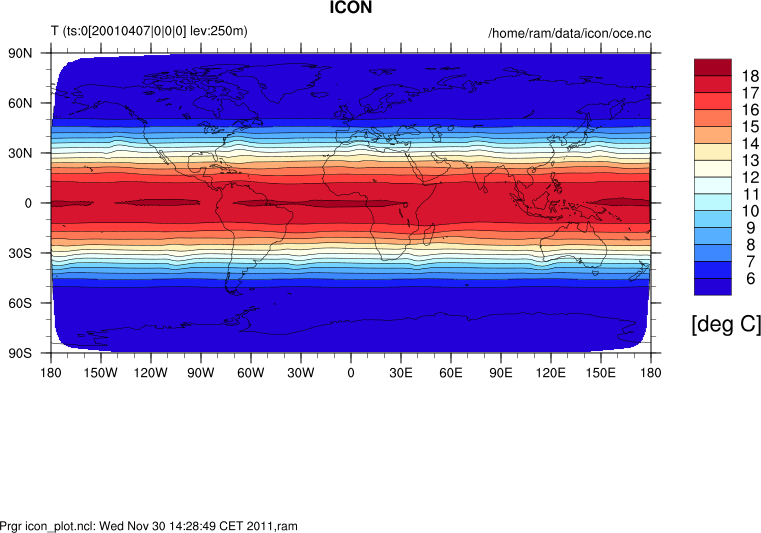
\includegraphics[width=0.95\linewidth]{pictures/contour_plot.png}
\caption{Example of contour plot}\label{fig:contour-plot}
\end{figure}

\subsubsection{Vector plots}
Use {\tt vecVars} instead of {\tt varName}. To adjust the length of the reference vector, use the variable {\tt vecRefLength}.

\begin{small}
\begin{verbatim}
ncl icon_plot.ncl 'vecVars="U V"' 'iFile="iFILENAME"' vecRefLength=0.01
\end{verbatim}
\end{small}

\begin{figure}[h!]%
\centering
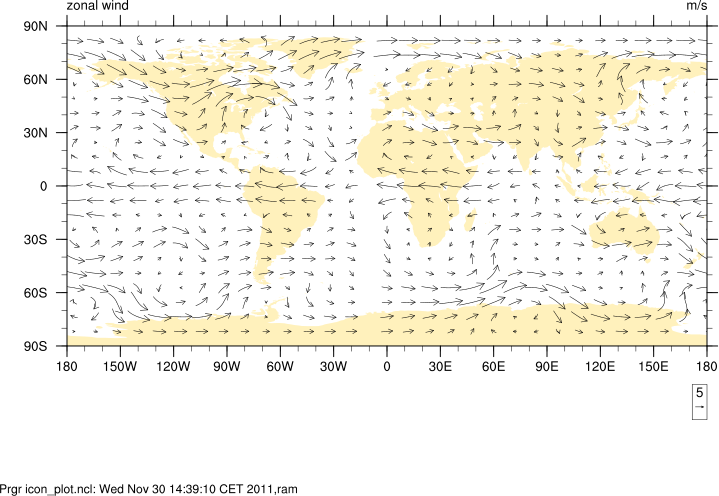
\includegraphics[width=0.95\linewidth]{pictures/vector_plot.png}
\caption{Example of vector plot}\label{fig:vector-plot}
\end{figure}

\subsubsection{Overlay of scalar and vector variables}
Contour and vector plots can be combined into a single plot by overlaying both. Following this approach, such an overlay plot will be created, if {\tt varName} and {\tt vecVars} are given: 

\begin{small}
\begin{verbatim}
ncl icon_plot.ncl 'varName="T"' 'iFile="iFILENAME"' 'vecVars="U V"'
\end{verbatim}
\end{small}

\begin{figure}[h!]%
\centering
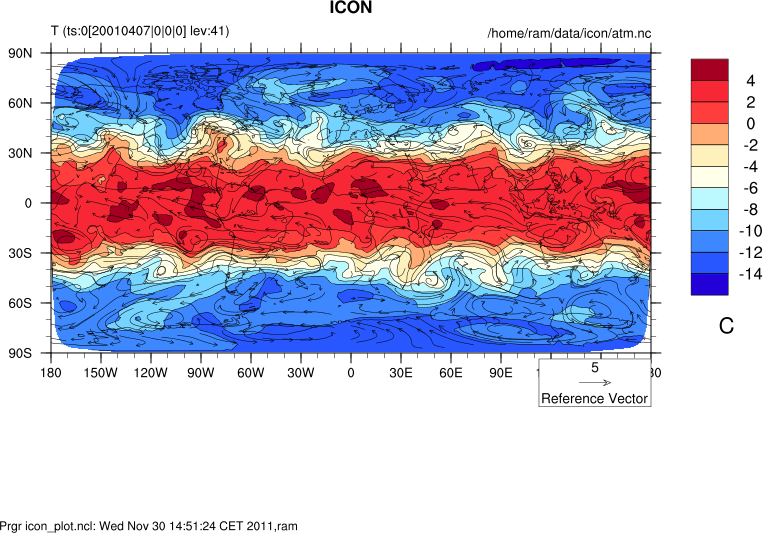
\includegraphics[width=0.95\linewidth]{pictures/overlay_plot.png}
\caption{Example of overlay plot}\label{fig:overlay-plot}
\end{figure}

\subsubsection{Vertical sections}
Data for sections have to be interpolated first. This is done internally and you do not have to care about it. Section plot are created, if a start and and end point of a section is given. For this purpose, the variables {\tt secLC} (section-left-corner) and {\tt secRC} (section-right-corner) have to be used. Theses variable have to be {\tt (lon,lat)} arrays like {\tt secLC=(/20.,30./)}.

Example call:

\begin{small}
\begin{verbatim}
ncl icon_plot.ncl 'varName="T"' 'iFile="iFILENAME"'  \
    'secLC=(/0,80/)' 'secRC=(/0,-80/)'
\end{verbatim}
\end{small}

{\tt secPoints} is an option to set the accuracy of the plot. The representing of the location of the section is suppressed by setting {\tt showSecMap=False}. Its default value is {\tt True}.

\begin{figure}[h!]%
\centering
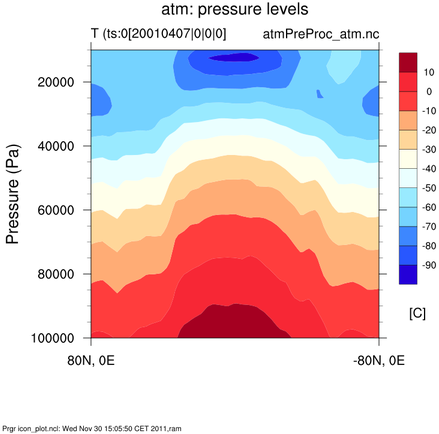
\includegraphics[width=0.95\linewidth]{pictures/vertsection_plot.png}
\caption{Example of vertical sections plot}\label{fig:vertsections-plot}
\end{figure}

\subsubsection{Display the ICON grid}
Set the parameter {\tt showGrid} to {\tt True} and for scalar variables, the ICON grid is represented instead of the contour plot. For large grids, this can take a long time.

\subsection{Regional plots}
Use the variables {\tt mapLLC} (map-Lower-Left-Corner) and {\tt mapURC} (map-Upper-Right-Corner) to select special regions of the earth. Here is a list of useful examples:

\begin{table}[htd]
\caption{Examples of useful regional plots}
\begin{center}
\begin{tabular}{lll}\hline
Trop. Atlantic &	{\tt 'mapLLC=(/-60, -25/)'}	& {\tt 'mapURC=(/ 25,25/)'}\\
North Polar	&{\tt 'mapLLC=(/-200, 20/)'}	& {\tt 'mapURC=(/160,90/)'}\\
North Atlantic	&{\tt 'mapLLC=(/-100,-15/)'}	& {\tt 'mapURC=(/ 35,65/)'}\\
Labrador/Panama	&{\tt 'mapLLC=(/-200, -5/)'}	 &{\tt 'mapURC=(/ 35,85/)'}\\
North Atlantic/Eurasia&	{\tt 'mapLLC=(/ -80, -5/)'}&	 {\tt 'mapURC=(/ 75,85/)'}\\
Asia	&{\tt 'mapLLC=(/ 20,-15/)'}	& {\tt 'mapURC=(/160,85/)'}\\\hline
\end{tabular}
\end{center}
\end{table}

\newpage

\subsection{Masking}
Masking can be done in two different ways:
\begin{enumerate}
\item Manually mask the data with CDO before running the plot scripts, i.e. use the ifthen operator or perform a division with the mask variable:
\begin{small}
\begin{verbatim}
 cdo div iconInput.nc -selname,mask_variable iconInput.nc maskedOutput.nc
\end{verbatim}
\end{small}
\item Let the plot script perform the masking using the NCL's mask function. For this purpose, the commandline variables {\tt maskName} and {\tt maskFile} have to be used. If the mask variable is part of the regular input file, {\tt maskFile} can be left out.
\end{enumerate}

Both methods have their pros and cons. Whereas the second methods works fine for all types of horizontal representation, the first produces better results for vertical cross sections.

\subsection{Data on other grids}
Although {\tt icon\_plot.ncl} is implemented for ICON, it can be used for data an regular grids, too. In this case, internal interpolation is not performed.

\subsection{All options}\label{all_options}
{\tt icon\_plot.ncl} has built-in documentation of all options. Use
\begin{small}
\begin{verbatim}
ncl icon_plot.ncl help=True 
\end{verbatim}
\end{small}

%MORE INFORMATION IN REDMINE!!!! (including graphics etc., ask Daniel for access)

\section{ncview/GrADS}
Ncview (\href{http://meteora.ucsd.edu/~pierce/ncview_home_page.html}{http://meteora.ucsd.edu/\~{}pierce/ncview\_home\_page.html}) and GrADS (\href{http://www.iges.org/grads/}{http://www.iges.org/grads/}) can be used after converting icon data sets to a regular grid. This can easily be done with cdo:
\begin{small}
\begin{verbatim}
cdo -P 8 -r remapnn,r180x90 icon.nc regular_icon.nc
\end{verbatim}
\end{small}
This uses nearest neighbor interpolation and hereby keeps the model values. When using a higher regular resolution the triangular icon grid keeps visible.

\section{Other Possibilities}
\begin{itemize}
\item GMT is useful, when the grid should be visualized.
\item ParaView is an alternative to display data on an unstructured grid. As a caveat, the model output has first to be converted into the vtk format.
\end{itemize}


\newpage
\subsection*{Discussion}

%This sction is for discussion only. Please add your notes, your name and date.
%Document last edited by \textit{Daniel Rieger} on \textit{26.11.2013}.\\
Document last edited by \textit{\krauti} on \textit{29.11.2013}.\\
Note: -


\chapter{ICON Namelists Overview}
%%%%%%%%%%%%%%%%%%%%%%%%%%%%%%%%%%%%%%%%%%%%%%%
% Progression Bar
% |=================>  |
% empty chapter        chapter finished
%%%%%%%%%%%%%%%%%%%%%%%%%%%%%%%%%%%%%%%%%%%%%%%

\section{Namelist Annotation}
Every ICON run generates annotated lists of namelist parameters during the setup. These lists are written to text files {\tt nml.atmo.log}, {\tt nml.cpl.log}, {\tt nml.ocean.log} and have the following form:

\begin{small}
\begin{verbatim}
NAMELIST IO_NML
    OUT_EXPNAME          'case4                        [...]' (truncated)
                         >> DEFAULT: 'IIIEEEETTTT      [...]' (truncated)
    OUT_FILETYPE         2
    LKEEP_IN_SYNC        F
    DT_DATA              43200.000000000000
                         >> DEFAULT: 21600.000000000000
    DT_DIAG              1728000.0000000000
                         >> DEFAULT: 86400.000000000000
\end{verbatim}
\end{small}

and so on.

The {\tt DEFAULT} annotation denotes all those parameters that have been modified by the user; in this case the default value of the namelist parameter is stated together with the modified value. All other namelist parameters are listed only with their default values.

\begin{landscape}
%% Because html converters don't know tabularnewline
\providecommand{\tabularnewline}{\\}
%%%%%%%%%%%%%%%%%%%%%%%%%%%%%% User specified LaTeX commands.
%\makeatletter

\newenvironment{longtab}
{
\begin{longtable}
{|>{\raggedright}p{4cm}
 |>{\raggedright}p{1.5cm}
 |>{\raggedright}p{1.5cm}
 |>{\raggedright}p{1cm}
 |>{\raggedright}p{8cm}
 |>{\raggedright}p{4cm}|}
\hline
Parameter& Type& Default& Unit& Description & Scope
\tabularnewline
\hline
\endhead
}
{
\hline
\end{longtable}
}

% ------------------------------------------------------
% new environment for documentation of namelist changes
% that are incompatible with former versions.
% ------------------------------------------------------

\newenvironment{changeitem}[3]
{
 \rule[-1em]{0.2ex}{4em}\hspace*{1em}%
 \begin{minipage}{9.95\textwidth}
 \begin{tabbing}
 \hspace*{3cm} \= ~ \kill
 \textcolor{red}{\emph{Change:}}         \> \textbf{#1} \\
 \textcolor{red}{\emph{Date of Change:}} \> \textbf{#2} \\
 \textcolor{red}{\emph{Revision:}}       \> \textbf{#3} \\
 \end{tabbing}
 \end{minipage}
}{\vspace*{1em}}


% ------------------------------------------------------
% new environment for short comments:
% ------------------------------------------------------

\newenvironment{note}{%
\begin{list}{}%
         {}%
         \item[\textbf{Note:} ] ~\\%
}{%
\end{list}
}


\section{ICON Namelists}

\subsection{Scripts, Namelist files and Programs}

Run scripts starting the programs for the grid generation and the
models are stored in run/. These scripts write namelist files containing
the specified Fortran namelists. Programs are stored in $<$ icon home$>$/build/$<$architecture$>$/bin/.


\begin{table}[htd]
\caption{Namelist files}
\begin{center}
\begin{tabular}{llll}\hline
\textbf{Namelist file} & \textbf{Purpose} & \textbf{Made by script} & \textbf{Used by program} \\\hline
NAMELIST\_GRAPH   & Generate graphs     & create\_global\_grids.run & grid\_command \\
NAMELIST\_GRID    & Generate grids      & create\_global\_grids.run & grid\_command \\
NAMELIST\_GRIDREF & Gen. nested domains & create\_global\_grids.run & grid\_command \\
NAMELIST\_ICON    & Run ICON models     & exp.<name>.run & control\_model   \\ \hline
\end{tabular}
\end{center}
\label{table:namelistfiles}
\end{table}

\newpage

\subsection{Namelist parameters}

The following subsections tabulate all available Fortran namelist
parameters by name, type, default value, unit, description, and scope:

\begin{itemize}
\item \emph{Type} refers to the type of the Fortran variable, in which the
value is stored: I=INTEGER, L=LOGICAL, R=REAL, C=character string
\item \emph{Default} is the preset value, if defined, that is assigned to
this parameter within the programs.
\item \emph{Unit} shows the unit of the control parameter, where applicable.
\item \emph{Description} explains in a few words the purpose of the parameter.
\item \emph{Scope} explains under which conditions the namelist parameter
has any effect, if its scope is restricted to specific settings of
other namelist parameters.
\end{itemize}
Information on the file, where the namelist is defined and used, is
given at the end of each table.


\section{Namelist parameters for grid generation}

\subsection{Namelist parameters defining the atmosphere grid}

%-----------------------------------------------------------------------------
% graph_ini:
%-----------------------------------------------------------------------------
\subsubsection{graph\_ini (NAMELIST\_GRAPH)}

\begin{longtab}

%\hline
\textbf{nroot}&
I&
2&
&
root subdivision of initial edges&
\tabularnewline

%\hline
\textbf{grid\_levels}&
I&
4&
&
number of edge bisections following the root subdivision&
\tabularnewline

%\hline
\textbf{lplane}&
L&
.FALSE.&
&
switch for generating a double periodic planar grid. The root level
consists of 8 triangles.&
\tabularnewline

\end{longtab}

Defined and used in: \verb+src/grid_generator/mo_io_graph.f90+

%-----------------------------------------------------------------------------
% grid_ini:
%-----------------------------------------------------------------------------
\subsubsection{grid\_ini (NAMELIST\_GRID)}

\begin{longtab}

%\hline
\textbf{nroot}&
I&
2&
&
root subdivision of initial edges&
\tabularnewline

%\hline
\textbf{grid\_levels}&
I&
4&
&
number of edge bisections following the root subdivision&
\tabularnewline

%\hline
\textbf{lplane}&
L&
.FALSE.&
&
switch for generating planar grid. The root level consists of 8 triangles.&
\tabularnewline

\end{longtab}

Defined and used in: \verb+src/grid_generator/mo_io_grid.f90+

%-----------------------------------------------------------------------------
% grid_options:
%-----------------------------------------------------------------------------
\subsubsection{grid\_options (NAMELIST\_GRID)}

\begin{longtab}

%\hline
\textbf{x\_rot\_angle}&
R&
0.0&
deg&
Rotation of the icosahedron about the x-axis (connecting the origin
and {[}0$^\circ$E, 0$^\circ$N])&
\tabularnewline

%\hline
\textbf{y\_rot\_angle} &
R&
0.0&
deg&
Rotation of the icosahedron about the y-axis (connecting the origin
and {[}90$^\circ$E, 0$^\circ$N), done after the rotation about the x-axis.&
\tabularnewline

%\hline
\textbf{z\_rot\_angle} &
R&
0.0&
deg&
rotation of the icosahedron about the z-axis (connecting the origin
and {[}0$^\circ$E, 90$^\circ$N), done after the rotation about the y-axis.&
\tabularnewline

%\hline
\textbf{itype\_optimize}&
I&
4&
&
Grid optimization type&
\tabularnewline
&
&
&
&
0: no optimization&
\tabularnewline
&
&
&
&
1: Heikes Randall&
\tabularnewline
&
&
&
&
2: equal area&
\tabularnewline
&
&
&
&
3: c-grid small circle&
\tabularnewline
&
&
&
&
4: spring dynamics&
\tabularnewline

%\hline
\textbf{l\_c\_grid} &
L &
.FALSE. &
&
C-grid constraint on last level&
\tabularnewline

%\hline
\textbf{maxlev\_optim} &
I &
100 &
&
Maximum grid level where the optimization is applied&
i\_type\_optimize = 1 or 4
\tabularnewline

%\hline
\textbf{beta\_spring} &
R &
0.90&
&
tuning factor for target grid length &
i\_type\_optimize = 4
\tabularnewline

\end{longtab}

Defined and used in: \verb+src/grid_generator/mo_io_grid.f90+


%-----------------------------------------------------------------------------
% plane_options:
%-----------------------------------------------------------------------------
\subsubsection{plane\_options (NAMELIST\_GRID)}

\begin{longtab}

%\hline
tria\_arc\_km &
R &
10.0 &
km&
length of triangle edge on plane&
lplane=.TRUE.
\tabularnewline

\end{longtab}

The number of grid points is generated by root level section and further
bisections. The double periodic root level consists of 8 triangles.
The spatial coordinates are $-1<=x<=1$, and $-\sqrt{3}/2<=y<=\sqrt{3}/2$.
Currently the planar option can only be used as an $f$-plane.

\noindent Defined and used in: \verb+src/grid_generator/mo_io_grid.f90+


%-----------------------------------------------------------------------------
% gridref_ini:
%-----------------------------------------------------------------------------
\subsubsection{gridref\_ini (NAMELIST\_GRIDREF)}

\begin{longtab}

%\hline
\textbf{grid\_root}&
I&
2&
&
root subdivision of initial edges&
\tabularnewline

%\hline
\textbf{start\_lev}&
I&
4&
&
number of edge bisections following the root subdivision&
\tabularnewline

%\hline
\textbf{n\_dom}&
I&
2&
&
number of logical model domains, including the global one&
\tabularnewline

%\hline
\textbf{n\_phys\_dom}&
I&
n\_dom&
&
number of physical model domains, may be larger than n\_dom (in this case, domain merging is applied)&
\tabularnewline

%\hline
\textbf{parent\_id}&
I(n\_phys\_ dom-1)&
i&
&
ID of parent domain (first entry refers to first nested domain; needs to be
specified only in case of more than one nested domain per grid level)&
\tabularnewline

%\hline
\textbf{logical\_id}&
I(n\_phys\_ dom-1)&
i+1&
&
logical grid ID of domain (first entry refers to first nested domain; needs to be
specified only in case of domain merging, i.e. n\_dom $<$ n\_phys\_dom) &
\tabularnewline

%\hline
\textbf{l\_plot}&
L&
.FALSE.&
&
produces GMT plots showing the locations of the nested domains&
\tabularnewline

%\hline
\textbf{l\_circ}&
L&
.TRUE.&
&
Create circular (.T.) or rectangular (.F.) refined domains &
\tabularnewline

%\hline
\textbf{l\_rotate}&
L&
.FALSE.&
&
Rotates center point into the equator in case of l\_circ = .FALSE. & lcirc=.FALSE.
\tabularnewline

%\hline
\textbf{write\_hierarchy}&
I&
1&
&
0: Output only computational grids \\
1: Output in addition parent grid of global model domain (required for computing physics on a reduced grid) \\
2: Output all grids back to level 0 (required for hierarchical search algorithms) &
\tabularnewline

%\hline
\textbf{bdy\_indexing\_depth}&
I&
max\_rlcell (=8)&
&
Number of cell rows along the lateral boundary of a model domain for which the refin\_ctrl
fields contain the distance from the lateral boundary; needs to be enlarged when lateral
boundary nudging is required for one-way nesting &
\tabularnewline

%\hline
\textbf{radius}&
R(n\_dom-1)&
30.&
deg&
radius of nested domain (first entry refers to first nested domain; needs to be
specified for each nested domain separately)&
lcirc=.TRUE.
\tabularnewline

%\hline
\textbf{hwidth\_lon}&
R(n\_dom-1)&
20.&
deg&
zonal half-width of refined domain (first entry refers to first nested domain; needs to be
specified for each nested domain separately)&
lcirc=.FALSE.
\tabularnewline

%\hline
\textbf{hwidth\_lat}&
R(n\_dom-1)&
20.&
deg&
meridional half-width of refined domain (first entry refers to first nested domain; needs to be
specified for each nested domain separately)&
lcirc=.FALSE.
\tabularnewline

%\hline
\textbf{center\_lon}&
R(n\_dom-1)&
90.&
deg&
center longitude of refined domain (first entry refers to first nested domain; needs to be
specified for each nested domain separately)&
\tabularnewline

%\hline
\textbf{center\_lat}&
R(n\_dom-1)&
30.&
deg&
center latitude of refined domain (first entry refers to first nested domain; needs to be
specified for each nested domain separately)&
\tabularnewline

\end{longtab}

Defined and used in: \verb+src/grid_generator/mo_gridrefinement.f90+


%-----------------------------------------------------------------------------
% gridref_metadata:
%-----------------------------------------------------------------------------
\subsubsection{gridref\_metadata (NAMELIST\_GRIDREF)}

\begin{longtab}

%\hline
number\_of\_grid\_used &
I(n\_dom+ 1)&
0&
&
sets the number of grid used in the netcdf header; the number of entries must be n\_dom+1
because the first number refers to the radiation grid &
\tabularnewline

%\hline
centre&
I&
0&
&
centre running the grid generator: 78 - edzw (DWD), 252 - MPIM &
\tabularnewline

%\hline
subcentre&
I&
0&
&
subcentre to be assigned by centre, usually 0 &
\tabularnewline

%\hline
outname\_style&
I&
1&
&
Output name style\\
1: Standard: \emph{iconR\textcolor{red}{X}B\textcolor{red}{XX}\_DOM\textcolor{red}{XX}.nc}\\
2: DWD: \emph{icon\_grid\_\textcolor{red}{XXXX}\_R\textcolor{red}{XX}B\textcolor{red}{XX}\_\textcolor{red}{X}.nc} &
\tabularnewline

\end{longtab}



%MMMMMMMMMMMMMMMMMMMMMMMMMMMMMMMMMMMMMMMMMMMMMMMMMMMMMMMMMMMMMMMMMMMMMMMMMMMMMM
%MMMMMMMMMMMMMMMMMMMMMMMMMMMMMMMMMMMMMMMMMMMMMMMMMMMMMMMMMMMMMMMMMMMMMMMMMMMMMM
%MMMMMMMMMMMMMMMMMMMMMMMMMMMMMMMMMMMMMMMMMMMMMMMMMMMMMMMMMMMMMMMMMMMMMMMMMMMMMM

\section{Namelist parameters defining the ICON model}

Namelist parameters for the ICON models are organized in several thematic
Fortran namelists controling the experiment, and the properties of
dynamics, transport, physics etc.


%------------------------------------------------------------------------------
% coupling_nml:
%------------------------------------------------------------------------------
\subsection{coupling\_nml}
\begin{longtab}

%\hline
name &
C &
blank &  &
short name of the coupling field &
\tabularnewline

%\hline
dt\_coupling &
I &
0 &
s &
coupling time step / coupling interval &
\tabularnewline

%\hline
dt\_model &
I &
0 &
s &
model time step &
\tabularnewline

%\hline
lag &
I &
0 &   &
offset to coupling event in number of model time steps &
\tabularnewline

%\hline
l\_time\_average &
L &
.FALSE. &  &
.TRUE.: time averaging between two coupling events &
\tabularnewline

%\hline
l\_time\_accumulation &
L &
.FALSE. &  &
.TRUE.: accumulation of coupling fields in time between two coupling events &
\tabularnewline

%\hline
l\_diagnostic &
L &
.FALSE. &  &
.TRUE.: simple diagnostics (min, max, avg) for coupling fields is switched on &
\tabularnewline

%\hline
l\_activated &
L &
.FALSE. &  &
.TRUE.: activate the coupling of the respective coupling field &
\tabularnewline

\end{longtab}

Defined and used in: \verb+src/namelists/mo_coupling_nml.f90+


%-----------------------------------------------------------------------------
% diffusion_nml: horizontal (numerical) diffusion
%-----------------------------------------------------------------------------
\subsection{diffusion\_nml}
\begin{longtab}

%\hline
\textbf{lhdiff\_temp}&
L& .TRUE. & &
Diffusion on the temperature field&
\tabularnewline

%\hline
\textbf{lhdiff\_vn}&
L& .TRUE. & &
Diffusion on the horizontal wind field&
\tabularnewline

%\hline
\textbf{lhdiff\_w}&
L& .TRUE. & &
Diffusion on the vertical wind field&
\tabularnewline

%\hline
hdiff\_order&
I&{4~(hydro)} \\ {5 (NH)}& &
Order of $\nabla$ operator for diffusion:\\
-1: no diffusion\\
2: $\nabla^{2}$ diffusion (not available for NH model on triangles!)\\
3: Smagorinsky $\nabla^{2}$ diffusion
(includes frictional heating for the hexagonal model if lhdiff\_temp=.TRUE.) &
\tabularnewline
& & & & 4: $\nabla^{4}$ diffusion&
\tabularnewline
& & & &
5: Smagorinsky $\nabla^{2}$ diffusion combined with $\nabla^{4}$
background diffusion as specified via hdiff\_efdt\_ratio&
\tabularnewline
& & & &
defaults: 2 for hexagonal model, 4 for hydrostatic triangular model, 5 for nonhydrostatic triangular NH model&
\tabularnewline
& & & & 24 or 42: $\nabla{2}$ diffusion from model top to a certain level
(cf. k2\_pres\_max and k2\_klev\_max below);
$\nabla^{4}$ for the lower levels.  &
24 and 42 currently allowed only in the hydrostatic atm model
(run\_nml:iequation = 1 or 2).
\tabularnewline

%\hline
itype\_vn\_diffu&
I& 1 & &
Reconstruction method used for Smagorinsky diffusion: \\
1: u/v reconstruction at vertices only \\
2: u/v reconstruction at cells and vertices& iequations=3, hdiff\_order=3 or 5
\tabularnewline

%\hline
itype\_t\_diffu&
I& 2 & &
Discretization of temperature diffusion: \\
1: $K_h \nabla^2 T$ \\
2: $\nabla \cdot (K_h \nabla T)$  & iequations=3, hdiff\_order=3 or 5
\tabularnewline

%\hline
k2\_pres\_max&
R& -99.& Pa &
Pressure level above which $\nabla^2$ diffusion is applied.&
hdiff\_order = 24 or 42, and run\_nml:iequation = 1 or 2.
\tabularnewline

%\hline
k2\_klev\_max&
I& 0&&
Index of the vertical level till which (from the model top)
$\nabla^2$ diffusion is applied.
If a positive value is specified for k2\_pres\_max,
k2\_klev\_max is reset accordingly during the initialization
of a model run.&
hdiff\_order = 24 or 42, and run\_nml:iequation = 1 or 2.
\tabularnewline

%\hline
hdiff\_efdt\_ratio&
R& 1.0 (hydro) \\ 36.0 (NH) & &
ratio of e-folding time to time step (or 2{*} time step when using
a 3 time level time stepping scheme) (only for triangles currently;
for triangular NH model, values above 30 are recommended when using hdiff\_order=5) &
\tabularnewline

%\hline
hdiff\_w\_efdt\_ratio&
R& 15.0  & &
ratio of e-folding time to time step for diffusion on vertical wind speed & iequations=3
\tabularnewline

%\hline
hdiff\_min\_efdt\_ratio&
R& 1.0 & &
minimum value of hdiff\_efdt\_ratio near model top & iequations=3  .AND. hdiff\_order=4
\tabularnewline

%\hline
hdiff\_tv\_ratio&
R& 1.0& &
Ratio of diffusion coefficients for temperature and normal wind: $T:v_{n}$&
\tabularnewline

%\hline
hdiff\_multfac&
R& 1.0& &
Multiplication factor of normalized diffusion coefficient for nested
domains&
n\_dom$>$1\tabularnewline

%\hline
\textbf{hdiff\_smag\_fac}&
R& 0.15 (hydro) \\ 0.015 (NH)& &
Scaling factor for Smagorinsky diffusion&
for triangles only with iequations=3, for hexagons with hdiff\_order=3
\tabularnewline

\end{longtab}

Defined and used in: \verb+src/namelists/mo_diffusion_nml.f90+


%-----------------------------------------------------------------------------
% dynamics_nml:
%-----------------------------------------------------------------------------
\subsection{dynamics\_nml}
This namelist is relevant if run\_nml:ldynamics=.TRUE.

\begin{longtab}

%\hline
\textbf{iequations}&
I& 1& &
Equations and prognostic variables. Use positive indices for the atmosphere
and negative indices for the ocean.&\tabularnewline
&&&&0: shallow water model&\tabularnewline
&&&&1: hydrostatic atmosphere, T&\tabularnewline
&&&&2: hydrostatic atm., $\theta \cdot$dp&\tabularnewline
&&&&3: non-hydrostatic atmosphere&\tabularnewline
&&&&-1: hydrostatic ocean&
\tabularnewline


%\hline
idiv\_method &
I& 1& &
Method for divergence computation:&
\tabularnewline
& & & & 1: Standard Gaussian integral. Hydrostatic atm.~model:
for unaveraged normal components,
Non-hydrostatic atm.~model: for averaged normal components &
\tabularnewline
& & & & 2: bilinear averaging of divergence& \tabularnewline

%\hline
divavg\_cntrwgt&
R& 0.5& &
Weight of central cell for divergence averaging&
idiv\_method= 2
\tabularnewline

%\hline
sw\_ref\_height &
R &  0.9* 2.94e4/g & m &
Reference height of shallow water model used for
linearization in the semi-implicit time stepping scheme&
\tabularnewline

%\hline
lcoriolis &
L & .TRUE.& &
Coriolis force&
\tabularnewline

\end{longtab}

Defined and used in: \verb+src/namelists/mo_dynamics_nml.f90+


%------------------------------ switches for ECHAM physics


%------------------------------------------------------------------------------
% echam_conv_nml:
%------------------------------------------------------------------------------
\subsection{echam\_conv\_nml}

\begin{longtab}

%\hline
\textbf{iconv}&
I & 1 &&
Choice of cumulus convection scheme.\par
1: Nordeng scheme\par
2: Tiedtke scheme\par
3: hybrid scheme &
iforcing = 2 .AND. lconv = .TRUE.
\tabularnewline

%\hline
ncvmicro&
I & 0 &&
Choice of convective microphysics scheme.&

iforcing = 2 .AND. lconv = .TRUE.
\tabularnewline

%\hline
lmfpen &
L& .TRUE.&&
Switch on penetrative convection.&
iforcing = 2 .AND. lconv = .TRUE.
\tabularnewline

%\hline
lmfmid &
L& .TRUE.&&
Switch on midlevel convection.&
iforcing = 2 .AND. lconv = .TRUE.
\tabularnewline

%\hline
lmfdd &
L& .TRUE.&&
Switch on cumulus downdraft.&
iforcing = 2 .AND. lconv = .TRUE.
\tabularnewline

%\hline
lmfdudv &
L& .TRUE.&&
Switch on cumulus friction.&
iforcing = 2 .AND. lconv = .TRUE.
\tabularnewline

%\hline
cmftau &
R & 10800. &&
Characteristic convective adjustment time scale.&
iforcing = 2 .AND. lconv = .TRUE.
\tabularnewline

%\hline
cmfctop &
R & 0.3 &&
Fractional convective mass flux (valid range [0,1])
across the top of cloud &
iforcing = 2 .AND. lconv = .TRUE.
\tabularnewline

%\hline
cprcon &
R & 1.0e-4 &&
Coefficient for determining conversion from cloud water to rain.&
iforcing = 2 .AND. lconv = .TRUE.
\tabularnewline

%\hline
cminbuoy &
R & 0.025 &&
Minimum excess buoyancy.&
iforcing = 2 .AND. lconv = .TRUE.
\tabularnewline

%\hline
entrpen &
R & 1.0e-4 &&
Entrainment rate for penetrative convection.&
iforcing = 2 .AND. lconv = .TRUE.
\tabularnewline

%\hline
dlev &
R & 3.e4 & Pa &
Critical thickness necessary for the onset of convective precipitation.&
iforcing = 2 .AND. lconv = .TRUE.
\tabularnewline

\end{longtab}

Defined and used in: \verb+src/namelists/mo_echam_conv_nml.f90+


\newpage

%------------------------------------------------------------------------------
% echam_phy_nml:
%------------------------------------------------------------------------------
\subsection{echam\_phy\_nml}

\begin{longtab}

\textbf{lrad} &
L& .TRUE.&&
Switch on radiation.& iforcing = 2
\tabularnewline

%\hline
\textbf{lvdiff} &
L& .TRUE.&&
Switch on turbulent mixing (i.e. vertical diffusion).&
iforcing = 2
\tabularnewline

%\hline
\textbf{lconv} &
L& .TRUE.&&
Switch on cumulus convection.& iforcing = 2
\tabularnewline

%\hline
\textbf{lcond} &
L& .TRUE.&&
Switch on large scale condensation.& iforcing = 2
\tabularnewline

%\hline
\textbf{icover} &
I& 1 &&
1 = diagnostic Sunquist cloud cover scheme, \par 2 = prognostic Tompkins cloud cover scheme.&
iforcing = 2\par
Note: icover = .TRUE. runs, but has not been evaluated (yet) in ICON.
\tabularnewline

%\hline
\textbf{lgw\_hines} &
L& .FALSE.&&
.TRUE. for atmospheric gravity wave drag by the Hines scheme&
iforcing = 2\par
\tabularnewline

%\hline
\textbf{lssodrag} &
L& .FALSE.&&
.TRUE. for subgrid scale orographic drag& iforcing = 2\par {\color{red}Not implemeted yet}
\tabularnewline

%\hline
\textbf{llandsurf} &
L& .FALSE.&&
.TRUE. for surface exchanges& iforcing = 2\par {\color{red}Not implemeted yet}
\tabularnewline

%\hline
\textbf{lice} &
L& .FALSE.&&
.TRUE. for sea-ice temperature calculation& iforcing = 2\par {\color{red}Not implemeted yet}
\tabularnewline

%\hline
\textbf{lmeltpond} &
L& .FALSE.&&
.TRUE. for calculation of meltponds& iforcing = 2\par {\color{red}Not implemeted yet}
\tabularnewline

%\hline
\textbf{lhd} &
L& .FALSE.&&
.TRUE. for hydrologic discharge model& iforcing = 2\par
{\color{red}Not implemeted yet}
\tabularnewline

%\hline
\textbf{lmlo} &
L& .FALSE.&&
.TRUE. for mixed layer ocean& iforcing = 2\par {\color{red}Not implemeted yet}
\tabularnewline

%\hline
\textbf{dt\_rad} &
R&
3600.&
s&
time interval of full radiation computation&
run\_nml/iforcing = iecham
\tabularnewline

%\hline
\end{longtab}

Defined and used in: \verb+src/namelists/mo_echam_phy_nml.f90+


%------------------------------------------------------------------------------
% gribout_nml:
%------------------------------------------------------------------------------
\subsection{gribout\_nml}
\begin{longtab}

%\hline
backgroundProcess&
I& 0 & &
Background process \\
- GRIB2 code table backgroundProcess.table &
filetype=2
\tabularnewline

%\hline
generatingCenter&
I& -1 & &
Output generating center. If this key is not set, center information is taken from the grid file\\
DWD: 78 \\
MPIMET: 98 \\
ECMWF: 98 &
filetype=2
\tabularnewline

%\hline
generatingProcess\par Identifier&
I(n\_dom)& 1 & &
generating Process Ident- ifier \\
- GRIB2 code table generatingProcessIdentifier.table &
filetype=2
\tabularnewline

%\hline
generatingSubcenter&
I& -1 & &
Output generating Subcenter. If this key is not set, subcenter information is taken from the grid file\\
DWD: 255\\
MPIMET: 232\\
ECMWF: 0 &
filetype=2
\tabularnewline

lspecialdate\_invar&
L& .FALSE. &&
SPecial reference date for invariant and climatological fields\\
.TRUE.: set special reference date 0001-01-01, 00:00\\
.FASLE.: no special reference date &
filetype = 2
\tabularnewline

%\hline
ldate\_grib\_act&
L& .TRUE. & &
GRIB creation date\\
.TRUE.: add creation date\\
.FALSE.: add dummy date &
filetype=2
\tabularnewline

%\hline
lgribout\_24bit&
L& .FALSE. & &
If TRUE, write thermodynamic fields $\rho$, $\theta_{v}$, $T$, $p$ with 24bit precision instead of 16bit &
filetype=2
\tabularnewline

%\hline
localDefinitionNumber&
I& 254 & &
local Definition Number\\
- GRIB2 code table grib2LocalSectionNumber.78.table &
filetype=2
\tabularnewline

%\hline
localNumberOfExperi- ment&
I& 1 & &
local Number of Experiment &
filetype=2
\tabularnewline

%\hline
numberOfForecastsIn- Ensemble&
I& -1 & &
Local definiton for ensemble products,
(only set if value changed from default) &
filetype=2
\tabularnewline

%\hline
perturbationNumber&
I& -1 & &
Local definiton for ensemble products,
(only set if value changed from default) &
filetype=2
\tabularnewline

%\hline
preset&
C& ''none'' & &
Setting this different to ''none'' enables a couple of defaults for
the other \texttt{gribout\_nml} namelist parameters. If, additionally, the
user tries to set any of these other parameters to a conflicting
value, an error message is thrown. 
Possible values are ''none'', ''deterministic'', ''ensemble''.
&
filetype=2
\tabularnewline


%\hline
productionStatusOfPro-\par cessedData&
I& 1 & &
Production status of data\\
- GRIB2 code table 1.3 &
filetype=2
\tabularnewline

%\hline
significanceOfReference- Time &
I& 1& &
Significance of reference time\\
- GRIB2 code table 1.2 &
filetype=2
\tabularnewline

%\hline
typeOfEnsembleForecast&
I& -1 & &
Local definiton for ensemble products
(only set if value changed from default) &
filetype=2
\tabularnewline

%\hline
typeOfGeneratingPro- cess&
I& 2 & &
Type of generating process \\
- GRIB2 code table 4.3 &
filetype=2
\tabularnewline

%\hline
typeOfProcessedData&
I& 1 & &
Type of data \\
- GRIB2 code table 1.4 &
filetype=2
\tabularnewline

%\hline
\end{longtab}

Defined and used in: \verb+src/namelists/mo_gribout_nml.f90+


%-------------------------------------------------------------------
% grid_nml: horizontal grid
%-------------------------------------------------------------------
\subsection{grid\_nml}
\begin{longtab}

%\hline
cell\_type&
I & 3& &
Cell type: not used &
\tabularnewline

%\hline
lplane &
L & .FALSE.& &
planar option&
\tabularnewline

%\hline
is\_plane\_torus &
L & .FALSE.& &
f-plane approximation on triangular grid &
\tabularnewline

%\hline
corio\_lat &
R & 0.0& deg&
Center of the f-plane is located at this geographical latitude &
lplane=.TRUE. and is\_plane\_torus=.TRUE.
\tabularnewline

%\hline
grid\_angular \_velocity &
R & Earth's & rad/s &
The angular velocity in rad per sec. &
\tabularnewline

%%\hline
%start\_lev &
%I & 4& &
%coarsest bisection level&
%\tabularnewline

%\hline
\textbf{l\_limited\_area} &
L & .FALSE.& & &
\tabularnewline

%\hline
grid\_rescale\_factor &
R & 1.0   &  &
The geometry and the timestep will be multiplied by this factor.\\
The angular velocity will be divided by this factor.
&
\tabularnewline

%\hline
\textbf{lfeedback} &
L(n\_dom) & .TRUE.& &
Specifies if feedback to parent grid is performed. Setting lfeedback(1)=.false. turns off feedback
for all nested domains; to turn off feedback for selected nested domains, set lfeedback(1)=.true.
and set ``.false." for the desired model domains&
n\_dom$>$1
\tabularnewline

%\hline
ifeedback\_type &
I & 2& &
1: incremental feedback \\ 2: relaxation-based feedback \\
Note: vertical nesting requires option 2 to run numerically stable over longer time periods & n\_dom$>$1
\tabularnewline

%\hline
start\_time &
R(n\_dom) & 0.   & s &
Time when a nested domain starts to be active (namelist entry is ignored for the global domain)
& n\_dom$>$1
\tabularnewline

%\hline
end\_time &
R(n\_dom) & 1.E30  & s &
Time when a nested domain terminates (namelist entry is ignored for the global domain)
& n\_dom$>$1
\tabularnewline

%\hline
patch\_weight &
R(n\_dom) & 0.& &
If patch\_weight is set to a value $>$ 0 for any of the first level child patches,
processor splitting will be performed, i.e. every of the first level child patches
gets a subset of the total number or processors corresponding to its patch\_weight.
A value of 0. corresponds to exactly 1 processor for this patch, regardless of
the total number of processors. For the root patch and higher level childs,
patch\_weight is not used. However, patch\_weight must be set to 0 for these patches
to avoid confusion.&
n\_dom$>$1
\tabularnewline

%\hline
lredgrid\_phys &
L & .FALSE.& &
If set to .true.  is calculated on a reduced grid (= one grid level higher) &
\tabularnewline

%\hline
\textbf{dynamics\_grid\_ filename} &
C & & &
Array of the grid filenames to be used by the dycore.
May contain the keyword \texttt{<path>} which will be substituted by
\texttt{model\_base\_dir}. &
\tabularnewline

%\hline
\textbf{dynamics\_parent\_ grid\_id} &
I & & &
Array of the indexes of the parent grid filenames, as described by the dynamics\_grid\_filename array.
Indexes start at 1, an index of 0 indicates no parent. &
\tabularnewline

%\hline
\textbf{radiation\_grid\_ filename} &
C & & &
Array of the grid filenames to be used for the radiation model.
Filled only if the radiation grid is different from the dycore grid.
May contain the keyword \texttt{<path>} which will be substituted by
\texttt{model\_base\_dir}.
&
\tabularnewline

%\hline
\textbf{dynamics\_radiation\_g rid\_link} &
I & & &
Array of the indexes linking the dycore grids, as described by the dynamics\_grid\_filename array,
and the radiation\_grid\_filename array. It provides the link index of the radiation\_grid\_filename,
for each entry of the dynamics\_grid\_filename array.
Indexes start at 1, an index of 0 indicates that the radiation grid is the same as the dycore grid.
Only needs to be filled when the radiation\_grid\_filename is defined. &
\tabularnewline

%\hline
create\_vgrid &
L & .FALSE. & &
.TRUE.: Write vertical grid files containing (\texttt{vct\_a}, \texttt{vct\_b}, \texttt{z\_ifc}, and \texttt{z\_ifv}. &
\tabularnewline

%\hline
vertical\_grid\_filename &
C (n\_dom) & & &
Array of filenames. These files contain the vertical grid definition (\texttt{vct\_a}, \texttt{vct\_b}, \texttt{z\_ifc}. &
\tabularnewline

\end{longtab}

Defined and used in: \verb+src/namelists/mo_grid_nml.f90+



%-------------------------------------------------------------------
% gridref_nml: grid refinement and nesting
%-------------------------------------------------------------------
\subsection{gridref\_nml}
\begin{longtab}

%\hline
grf\_intmethod\_c&
I& 2& &
Interpolation method for grid refinement (cell-based dynamical variables):&
n\_dom$>$1\tabularnewline
& & & & 1: parent-to-child copying & \tabularnewline
& & & & 2: gradient-based interpolation & \tabularnewline

%\hline
grf\_intmethod\_ct&
I& 2& &
Interpolation method for grid refinement (cell-based tracer variables):&
n\_dom$>$1\tabularnewline
& & & & 1: parent-to-child copying & \tabularnewline
& & & & 2: gradient-based interpolation & \tabularnewline

%\hline
grf\_intmethod\_e&
I& 6& &
Interpolation method for grid refinement (edge-based variables):&
n\_dom$>$1\tabularnewline
& & & & 1: inverse-distance weighting (IDW) & \tabularnewline
& & & & 2: RBF interpolation & \tabularnewline
& & & & 3: combination gradient-based / IDW & \tabularnewline
& & & & 4: combination gradient-based / RBF & \tabularnewline
& & & & 5/6: same as 3/4, respectively, but direct interpolation of mass fluxes along nest interface edges & \tabularnewline

%\hline
grf\_velfbk&
I& 1& & Method of velocity feedback:&
n\_dom$>$1\tabularnewline
& & & & 1: average of child edges 1 and 2 & \tabularnewline
& & & & 2: 2nd-order method using RBF interpolation & \tabularnewline

%\hline
grf\_scalfbk&
I& 2& & Feedback method for dynamical scalar variables ($T, p_{sfc}$):&
n\_dom$>$1\tabularnewline
& & & & 1: area-weighted averaging & \tabularnewline
& & & & 2: bilinear interpolation & \tabularnewline

%\hline
grf\_tracfbk&
I& 2& & Feedback method for tracer variables:&
n\_dom$>$1\tabularnewline
& & & & 1: area-weighted averaging & \tabularnewline
& & & & 2: bilinear interpolation & \tabularnewline

%\hline
grf\_idw\_exp\_e12&
R& 1.2& &
exponent of generalized IDW function for child edges 1/2 &
n\_dom$>$1\tabularnewline

%\hline
grf\_idw\_exp\_e34&
R& 1.7& &
exponent of generalized IDW function for child edges 3/4 &
n\_dom$>$1\tabularnewline

%\hline
rbf\_vec\_kern\_grf\_e&
I& 1& &
RBF kernel for grid refinement (edges):&
n\_dom$>$1\tabularnewline
& & & & 1: Gaussian & \tabularnewline
& & & & 2: $1/(1+r^{2})$ & \tabularnewline
& & & & 3: inverse multiquadric & \tabularnewline

%\hline
rbf\_scale\_grf\_e&
R& 0.5& &
RBF scale factor for grid refinement (edges)&
n\_dom$>$1\tabularnewline

%\hline
denom\_diffu\_t&
R& 135& &
Deniminator for lateral boundary diffusion of temperature&
n\_dom$>$1\tabularnewline

%\hline
denom\_diffu\_v&
R& 200& &
Deniminator for lateral boundary diffusion of velocity&
n\_dom$>$1\tabularnewline

%\hline
l\_mass\_consvcorr&
L& .FALSE.& &
.TRUE.: Apply mass conservation correction in feedback routine &
n\_dom$>$1\tabularnewline

%\hline
l\_density\_nudging &
L& .FALSE.& &
.TRUE.: Apply density nudging near lateral nest boundary if grf\_intmethod\_e $\le$ 4&
n\_dom$>$1 .AND. lfeedback = .TRUE. \tabularnewline

\hline
fbk\_relax\_timescale &
R & 10800& &
Relaxation time scale for feedback &
n\_dom>1 .AND. lfeedback = .TRUE. .AND. ifeedback\_type = 2 \tabularnewline

\end{longtab}

Defined and used in: \verb+src/namelists/mo_gridref_nml.f90+


%------------------------------------------------------------------------------
% gw_hines_nml:
%------------------------------------------------------------------------------
\subsection{gw\_hines\_nml (Scope: lgw\_hines = .TRUE. in echam\_phy\_nml)}

\begin{longtab}

%\hline
lheatcal    &
L           &
.FALSE.     &&
.TRUE.: compute drag, heating rate and diffusion coefficient from the dissipation of gravity waves&
\tabularnewline
&&&&
.FALSE.: compute drag only &
\tabularnewline

%\hline
emiss\_lev  &
I           &
10          &&
Index of model level, counted from the surface, from which the gravity wave spectra are emitted &
\tabularnewline

%\hline
rmscon      &
R           &
1.0         &
m/s         &
Root mean square gravity wave wind at the emission level &
\tabularnewline

%\hline
kstar       &
R           &
5.0e-5      &
1/m         &
Typical gravity wave horizontal wavenumber &
\tabularnewline

%\hline
m\_min      &
R           &
0.0         &
1/m         &
Minimum bound in  vertical wavenumber &
\tabularnewline

%\hline
lrmscon\_lat &
L            &
.FALSE.      &
             &
.TRUE.:  use latitude dependent rms wind &
\tabularnewline
&&&& - |latitude| $>$= lat\_rmscon: use rmscon &
\tabularnewline
&&&& - |latitude| $<$= lat\_rmscon\_eq: use rmscon\_eq &
\tabularnewline
&&&& - lat\_rmscon\_eq $<$ |latitude| $<$ lat\_rmscon: use linear interpolation between rmscon\_eq and rmscon &
\tabularnewline
&&&& .FALSE.: use globally constant rms wind rmscon &
\tabularnewline

%\hline
lat\_rmscon\_eq &
R               &
5.0             &
deg N           &
rmscon\_eq is used equatorward of this latitude &
lrmscon\_lat = .TRUE.
\tabularnewline

%\hline
lat\_rmscon     &
R               &
10.0            &
deg N           &
rmscon is used polward of this latitude &
lrmscon\_lat = .TRUE.
\tabularnewline

%\hline
rmscon\_eq      &
R               &
1.2             &
m/s             &
is used equatorward of latitude lat\_rmscon\_eq &
lrmscon\_lat = .TRUE.
\tabularnewline

\end{longtab}

Defined and used in: \verb+src/namelists/mo_gw_hines_nml.f90+


%-----------------------------------------------------------------------------
% ha_dyn_nml: hydrostatic atm dynamics
%-----------------------------------------------------------------------------
\subsection{ha\_dyn\_nml}

This namelist is relevant if
run\_nml:ldynamics=.TRUE.
and dynamics\_nml:iequations=IHS\_ATM\_TEMP or IHS\_ATM\_THETA.

\begin{longtab}

%\hline
\textbf{itime\_scheme}&
I& 4& &
Time integration scheme:& \tabularnewline
& & & & 11: pure advection (no dynamics)& \tabularnewline
& & & & 12: 2 time level semi implicit (not yet implemented)&
\tabularnewline
& & & & 13: 3 time level explicit&
\tabularnewline
& & & & 14: 3 time level with semi implicit correction&
\tabularnewline
& & & & 15: standard 4th-order Runge-Kutta method (4-stage)&
\tabularnewline
& & & & 16: SSPRK(5,4) scheme (5-stage)&
\tabularnewline

%\hline
ileapfrog\_startup&
I& 1& &
How to integrate the first time step when the leapfrog scheme
is chosen. 1 = Euler forward; 2 = a series of sub-steps. &
itime\_scheme= 13 or 14 \tabularnewline

%\hline
asselin\_coeff&
R& 0.1& &
Asselin filter coefficient&
itime\_scheme= 13 or 14 \tabularnewline

%\hline
si\_2tls &
R & 0.6 & &
weight of time step n+1. Valid range: [0,1] &
itime\_scheme=12\tabularnewline

%\hline
si\_expl\_scheme &
I & 2 & &
scheme for the explicit part used in the 2 time level
semi-implicit time stepping scheme. 1 = Euler forward;
2 = Adams-Bashforth 2nd order &
itime\_scheme=12\tabularnewline

%\hline
si\_cmin&
R & 30.0 & m/s&
semi implicit correction is done for eigenmodes with speeds larger
than si\_cmin&
itime\_scheme=14 and lsi\_3d=.FALSE.\tabularnewline

%\hline
si\_coeff&
R & 1.0 & &
weight of the semi implicit correction&
itime\_scheme=14 \tabularnewline

%\hline
si\_offctr&
R & 0.7 & &
&
itime\_scheme=14 \tabularnewline

%\hline
si\_rtol &
R & 1.0e-3 & &
relative tolerance for GMRES solver&
itime\_scheme=14 \tabularnewline

%\hline
lsi\_3d&
L& .FALSE.& &
3D GMRES solver or decomposistion into 2D problems&
lshallow\_water=.FALSE. and itime\_scheme=14\tabularnewline
%\hline

%\hline
\textbf{ldry\_dycore} &
L & .TRUE. & &
Assume dry atmosphere &
iequations$\in$\{1,2\}
\tabularnewline

%\hline
\textbf{lref\_temp} &
L & .FALSE. & &
Set a background temperature profile as base state
when computing the pressure gradient force &
iequations$\in$\{1,2\}
\tabularnewline

\end{longtab}


%------------------------------------------------------------------------------
% initicon_nml
%------------------------------------------------------------------------------
\subsection{initicon\_nml}

\begin{longtab}

%\hline
\textbf{init\_mode}&
I & 1& &
1: start from DWD analysis \\
2: start from IFS analysis \\
3: combined mode: IFS atm + GME soil \\
4: start from COSMO-DE forecast &
\tabularnewline

dt\_iau&
R & 10800 & s &
Time interval during which an incremental analysis update (IAU) is performed &
init\_mode=5
\tabularnewline

%\hline
type\_iau\_wgt&
I & 1 &  &
Weighting function for performing IAU\\
1: Top-Hat\\
2: SIN2 &
init\_mode=5
\tabularnewline

%\hline
\textbf{nlevsoil\_in}&
I & 4 & &
number of soil levels of input data&
init\_mode=2
\tabularnewline

%\hline
zpbl1 &
R & 500.0& m&
bottom height (AGL) of layer used for gradient computation&
\tabularnewline

%\hline
zpbl2 &
R & 1000.0& m&
top height (AGL) of layer used for gradient computation&
\tabularnewline

%\hline
l\_sst\_in&
L & .TRUE.& &
Logical switch. If true, the surface temperature of the water sea points is initialized
with the SST provided in the ifs2icon file. If false, it is initialized with the skin
temperature. If the SST is not provided in the ifs2icon file,l\_sst\_in is reset to false.  &
init\_mode=2
\tabularnewline

%\hline
lread\_ana&
L & .TRUE.& &
If .FALSE., ICON is started from first guess only. Analysis field is not required, and skipped if provided. &
init\_mode=1,3
\tabularnewline


%\hline
l\_coarse2fine\_mode&
L(max\_ dom) & .FALSE.& &
If true, apply corrections for coarse-to-fine mesh interpolation to wind and temperature &
\tabularnewline

%\hline
\textbf{ifs2icon\_filename}&
C &
&
&
Filename of IFS2ICON input file, default
''\texttt{<path>ifs2icon\_R<nroot>B<jlev>\_DOM <idom>.nc}''.
May contain the keywords \texttt{<path>} which will be substituted by
\texttt{model\_base\_dir}, as well as \texttt{nroot}, \texttt{jlev},
and \texttt{idom} defining the current patch. & init\_mode=2
\tabularnewline

%\hline
\textbf{dwdfg\_filename}&
C &
&
&
Filename of DWD first-guess input file, default
''\texttt{<path>dwdFG\_R<nroot>B<jlev>\_DOM <idom>.nc}''.
May contain the keywords \texttt{<path>} which will be substituted by
\texttt{model\_base\_dir}, as well as \texttt{nroot}, \texttt{jlev},
and \texttt{idom} defining the current patch. & init\_mode=1,3
\tabularnewline

%\hline
\textbf{dwdana\_filename}&
C &
&
&
Filename of DWD analysis input file, default
''\texttt{<path>dwdana\_R<nroot>B<jlev>\_DOM
<idom>.nc}''.
May contain the keywords \texttt{<path>} which will be substituted by
\texttt{model\_base\_dir}, as well as \texttt{nroot}, \texttt{jlev},
and \texttt{idom} defining the current patch. & init\_mode=1
\tabularnewline

%\hline
\textbf{filetype} &
I& -1 (undef.)& &
One of CDI's FILETYPE\_XXX constants.
Possible values: 2 (=FILETYPE\_GRB2), 4 (=FILETYPE\_NC2).
If this parameter has not been set, we try to determine the file type by its extension "*.grb*" or ".nc".
&
\tabularnewline


%\hline
\textbf{ana\_varlist} &
C& & &
List of mandatory analysis fields that must be present in the analysis file. If these fields cannot be found in the analysis
file, the model aborts. For all other analysis fields, the FG-fields will serve as fallback position.
& init\_mode=1
\tabularnewline


%\hline
\textbf{ana\_varnames\_map\_ file} &
C& & &
Dictionary file which maps internal variable names onto
GRIB2 shortnames or NetCDF var names.
This is a text file with two columns separated by whitespace, where
left column: ICON variable name, right column: GRIB short name.
&
\tabularnewline

\end{longtab}

Defined and used in: \verb+src/namelists/mo_initicon_nml.f90+


%------------------------------------------------------------------------------
% interpol_nml: horizontal interpolation/reconstruction
%------------------------------------------------------------------------------
\subsection{interpol\_nml}
\begin{longtab}

%\hline
l\_intp\_c2l&
L& .TRUE.& &
If .TRUE. directly interpolate scalar variables from cell centers to
lon-lat points, otherwise do gradient interpolation and
reconstruction.&
\tabularnewline

%\hline
l\_mono\_c2l&
L& .TRUE.& &
Monotonicity can be enforced by demanding that the interpolated
value is not higher or lower than the stencil point values.&
\tabularnewline

%\hline
llsq\_high\_consv&
L& .TRUE.& &
conservative (T) or non-conservative (F) least-squares reconstruction for high order transport&
\tabularnewline

%\hline
lsq\_high\_ord&
I& 3& &
polynomial order for high order reconstruction& \tabularnewline
& & & & 1: linear & ihadv\_tracer=4 \tabularnewline
& & & & 2: quadratic & \tabularnewline
& & & & 30: cubic (no $3^{rd}$ order cross deriv.) & \tabularnewline
& & & & 3: cubic & \tabularnewline

%\hline
llsq\_lin\_consv&
L& .FALSE.& &
conservative (T) or non-conservative (F) least-squares reconstruction for 2nd order (linear) transport&
\tabularnewline

%\hline
nudge\_efold\_width&
R& 2.5& &
e-folding width (in units of cell rows) for lateral boundary nudging coefficient &
\tabularnewline

%\hline
nudge\_max\_coeff&
R& 0.02& &
Maximum relaxation coefficient for lateral boundary nudging&
\tabularnewline

%\hline
nudge\_zone\_width&
I& 8& &
Total width (in units of cell rows) for lateral boundary nudging zone. 
If < 0 the patch boundary\_depth\_index is used. &
\tabularnewline

%\hline
rbf\_dim\_c2l&
I& 10& &
stencil size for direct lon-lat interpolation:
 4 = nearest neighbor,
13 = vertex stencil,
10 = edge stencil.&
\tabularnewline

%\hline
rbf\_scale\_mode\_ll&
I& 2& &
Specifies, how the RBF shape parameter is
determined for lon-lat interpolation.
1 : lookup table based on grid level (default)
2 : determine automatically.
So far, this routine only estimates the smallest value for the shape parameter for which the Cholesky is likely to succeed in floating point arithmetic.
&
\tabularnewline

%\hline
rbf\_vec\_kern\_c&
I& 1& &
Kernel type for reconstruction at cell centres:& \tabularnewline
& & & & 1: Gaussian & \tabularnewline
& & & & 3: inverse multiquadric & \tabularnewline

%\hline
rbf\_vec\_kern\_e&
I& 3& &
Kernel type for reconstruction at edges:& \tabularnewline
& & & & 1: Gaussian & \tabularnewline
& & & & 3: inverse multiquadric & \tabularnewline

%\hline
rbf\_vec\_kern\_ll&
I& 1& &
Kernel type for reconstruction at lon-lat-points:& \tabularnewline
& & & & 1: Gaussian & \tabularnewline
& & & & 3: inverse multiquadric & \tabularnewline

%\hline
rbf\_vec\_kern\_v&
I& 1& &
Kernel type for reconstruction at vertices:& \tabularnewline
& & & & 1: Gaussian & \tabularnewline
& & & & 3: inverse multiquadric & \tabularnewline

%\hline
rbf\_vec\_scale\_c&
R(n\_dom)& resolution-dependent& &
Scale factor for RBF reconstruction at cell centres&
\tabularnewline

%\hline
rbf\_vec\_scale\_e&
R(n\_dom)& resolution-dependent& &
Scale factor for RBF reconstruction at edges&
\tabularnewline

%\hline
rbf\_vec\_scale\_v&
R(n\_dom)& resolution-dependent& &
Scale factor for RBF reconstruction at vertices&
\tabularnewline

\end{longtab}

Defined and used in: \verb+src/namelists/mo_interpol_nml.f90+


%------------------------------------------------------------------------------
% io_nml:
%------------------------------------------------------------------------------
\subsection{io\_nml}
\begin{longtab}

%\hline
lkeep\_in\_sync&
L& .FALSE. & &
Sync output stream with file on disk after each timestep&
\tabularnewline

%\hline
dt\_diag&
R& 86400. & &
diagnostic integral output interval &
\tabularnewline


%\hline
\textbf{dt\_checkpoint}&
R& 2592000 & s&
Time interval for writing restart files.
Note that if the value of dt\_checkpoint resulting from
model default or user's specification is longer than time\_nml:dt\_restart,
it will be reset (by the model) to dt\_restart so
that at least one restart file is generated during the restart cycle.
&
\texttt{output /= "none"} (\texttt{run\_nml})
\tabularnewline

%\hline
inextra\_2d&
I &
0&&
Number of extra 2D Fields for diagnostic/debugging output. &
iequations = 3 {\color{red}(to be done for 1, 2)}
\tabularnewline
%\hline
inextra\_3d&
I &
0&&
Number of extra 3D Fields for diagnostic/debugging output. &
iequations = 3 {\color{red}(to be done for 1, 2)}
\tabularnewline

%\hline
lflux\_avg&
L& .TRUE. & &
if .FALSE. the output fluxes are accumulated  \\
 from the beginning of the run                \\
if .TRUE. the output fluxes are average values\\
 from the beginning of the run, except of     \\
 TOT\_PREC that would be accumulated &
iequations=3\\
iforcing=3
\tabularnewline

%\hline
itype\_pres\_msl&
I& 1 & &
Specifies method for computation of mean sea level pressure (and geopotential at
pressure levels below the surface). \\
1: GME-type extrapolation, \\
2: stepwise analytical integration, \\
3: current IFS method, \\
4: IFS method with consistency correction
&
\tabularnewline

%\hline
itype\_rh&
I& 1 & &
Specifies method for computation of relative humidity \\
1: WMO-type: water only (e\_s=e\_s\_water), \\
2: IFS-type: mixed phase (water and ice), \\
3: IFS-type with clipping ($\mathrm{rh}\leq100$)
&
\tabularnewline

%\hline
 output\_nml\_dict &
C&' '& &
 File containing the mapping of variable names to the internal ICON names.
 May contain the keyword \texttt{<path>} which will be substituted by
 \texttt{model\_base\_dir}.\\
 The format of this file: \\
 One mapping per line, first the name as given in the \texttt{ml\_varlist},
 \texttt{hl\_varlist}, \texttt{pl\_varlist} or \texttt{il\_varlist}
 of the \texttt{output\_nml} namelists, then the internal ICON name,
 separated by an arbitrary number of blanks.
 The line may also start and end with an arbitrary number of blanks.
 Empty lines or lines starting with \# are treated as comments. \\
 Names not covered by the mapping are used as they are.
&
\texttt{output\_nml} namelists
\tabularnewline

%\hline
 netcdf\_dict &
C&' '& &
 File containing the mapping from internal names to names written to NetCDF.
 May contain the keyword \texttt{<path>} which will be substituted by
 \texttt{model\_base\_dir}.\\
 The format of this file: \\
 One mapping per line, first the name written to NetCDF,
 then the internal name, separated by an arbitrary number of blanks
 (\emph{inverse to the definition of \emph{output\_nml\_dict}}).
 The line may also start and end with an arbitrary number of blanks.
 Empty lines or lines starting with \# are treated as comments. \\
 Names not covered by the mapping are output as they are. \\
 Note that the specification of output variables, e.\,g.\ in
 \texttt{ml\_varlist}, is independent from this renaming, see
 the namelist parameter \texttt{varnames\_map\_file} for this.
&
\texttt{output\_nml} namelists,
NetCDF output
\tabularnewline

%\hline
lzaxis\_reference&
L& .TRUE. & &
FALSE: use vertical axis ZAXIS\_HYBRID for 3D atmospheric fields\\
TRUE: use vertical axis ZAXIS\_REFERENCE for 3D atmospheric fields &
will be removed after some testing phase
\tabularnewline

%\hline
\end{longtab}

Defined and used in: \verb+src/namelists/mo_io_nml.f90+


%------------------------------------------------------------------------------
% les_nml:
%------------------------------------------------------------------------------
\subsection{les\_nml (parameters for LES turbulence scheme; valid for inwp\_turb=5)}

\begin{longtab}

%\hline
sst & R & 300 & K &
sea surface temperature for idealized LES simulations &
nh\_test\_name=CBL, RICO\\
isrfc\_type=5,4
\tabularnewline

%\hline
shflx & R & -999 & Km/s &
Kinematic sensible heat flux at surface &
isrfc\_type = 2
\tabularnewline

%\hline
lhflx & R & -999 & m/s &
Kinematic latent heat flux at surface &
isrfc\_type = 2
\tabularnewline

%\hline
isrfc\_type & I & 1 &  &
surface type \\
1 = TERRA land physics \\
2 = fixed surface fluxes \\
3 = fixed buoyancy fluxes \\
4 = RICO test case \\
5 = fixed SST &
\tabularnewline

%\hline
ufric & R & -999 & m/s &
friction velocity for idealized LES simulations &
\tabularnewline

%\hline
is\_dry\_cbl & L & .FALSE. &  &
switch for dry convective boundary layer simulations &
\tabularnewline

%\hline
karman\_constant & R & 0.4 &  &
von Karman constant &
\tabularnewline

%\hline
smag\_constant & R & 0.12 &  &
Smagorinsky constant &
\tabularnewline

%\hline
turb\_prandtl & R & 0.333333 &  &
turbulent Prandtl number &
\tabularnewline

%\hline
bflux & R & -999 &  m$^2$/s$^3$ &
buoyancy flux for idealized LES simulations (Stevens 2007) &
isrfc\_type=3
\tabularnewline

%\hline
tran\_coeff & R & -999 &  m/s &
transfer coefficient near surface for idealized LES simulation (Stevens 2007)&
isrfc\_type=3
\tabularnewline

%\hline
vert\_scheme\_type & I & 2 &   &
type of time integration scheme in vertical diffusion \\
1 = explicit \\
2 = fully implicit \\ &
\tabularnewline

%\hline
sampl\_freq\_sec & R & 60 & s  &
sampling frequency in seconds for statistical (1D and 0D) output &
\tabularnewline

%\hline
avg\_interval\_sec & R & 900 & s  &
(time) averaging interval in seconds for 1D statistical output &
\tabularnewline

%\hline
expname & C & ICOLES &   &
expname to name the statistical output file &
\tabularnewline

%\hline
ldiag\_les\_out & L & .TRUE. &   &
Control for the statistical output in LES mode &
\tabularnewline

\end{longtab}

Defined and used in: \verb+src/namelists/mo_les_nml.f90+


%------------------------------------------------------------------------------
% limarea_nml:
%------------------------------------------------------------------------------
\subsection{limarea\_nml (Scope: l\_limited\_area=1 in grid\_nml)}

\begin{longtab}

%\hline
\textbf{itype\_latbc}&
I & 0& &
Type of lateral boundary nudging. Nudge from\\
0: the initial data,\\
1: IFS data analysis/forecast (if \texttt{init\_mode}=4, we take COSMO-DE data),\\
2: ICON output data (with the identical 3d grid)&
\tabularnewline

%\hline
\textbf{dtime\_latbc}&
R &
10800.0& s
&
Time difference between two consecutive boundary data.
&
itype\_latbc $\ge$ 1
\tabularnewline

%\hline
\textbf{nlev\_latbc}&
I &
0& s
&
Number of vertical levels in boundary data.
&
itype\_latbc $\ge$ 1
\tabularnewline

%\hline
\textbf{latbc\_filename}&
C &
&
&
Filename of boundary data input file, default:\\
''\texttt{prepiconR<nroot>B<jlev>\_<y><m><d><h>.nc}''.
\texttt{<y>}, \texttt{<m>}, \texttt{<d>}, and \texttt{<h>} 
will be automatically replaced during the run-time. In case
the time span between two consecutive boundary data is less than 1 hour, 
one can use \texttt{<min>} and \texttt{<sec>}.
These files must be located in
the \texttt{latbc\_path} directory.
&
itype\_latbc $\ge$ 1
\tabularnewline

%\hline
\textbf{latbc\_path}&
C &
&
&
Absolute path to boundary data.
&
itype\_latbc $\ge$ 1
\tabularnewline


\end{longtab}

Defined and used in: \verb+src/namelists/mo_limarea_nml.f90+


%------------------------------------------------------------------------------
% nwp_lnd_nml:
%------------------------------------------------------------------------------
\subsection{lnd\_nml}

\begin{longtab}

nlev\_snow &
I&
2&
&
number of snow layers\\
for {\tt lmulti\_snow=.true.}&
lmulti\_snow=.true.
\tabularnewline
%\hline
\textbf{ntiles} &
I&
1&
&
number of tiles&
\tabularnewline

%\hline
\textbf{lsnowtile} &
L&
.FALSE.&
&
.TRUE.: consider snow-covered and snow-free tiles separately &
ntiles$>$1
\tabularnewline

%\hline
frlnd\_thrhld &
R&
0.05&
&
fraction threshold for creating a land grid point &
ntiles$>$1
\tabularnewline

%\hline
frlake\_thrhld &
R&
0.05&
&
fraction threshold for creating a lake grid point &
ntiles$>$1
\tabularnewline
%\hline
frsea\_thrhld &
R&
0.05&
&
fraction threshold for creating a sea grid point &
ntiles$>$1
\tabularnewline

%\hline
frlndtile\_thrhld &
R&
0.05&
&
fraction threshold for retaining the respective tile for a grid point&
ntiles$>$1
\tabularnewline

\textbf{lmulti\_snow} &
L&
.TRUE.&
&
.TRUE. for use of multi-layer snow model&
\tabularnewline

%\hline
max\_toplaydepth &
R &
0.25&
m &
maximum depth of uppermost snow layer & lmulti\_snow=.TRUE.
\tabularnewline

%\hline
idiag\_snowfrac &
I & 1 &  & Type of snow-fraction diagnosis:\\ 
1 = based on SWE only\\
2--4 = more advanced experimental methods &
\tabularnewline

%\hline
itype\_lndtbl &
I & 1 &  & Table values used for associating surface parameters to land-cover classes: \\
1 = defaults from extpar (GLC2000 and GLOBCOVER2009)\\
2 = Tuned version based on IFS values for globcover classes (GLOBCOVER2009 only)\\
3 = even more tuned version (EXPERIMENTAL!!, GLOBCOVER2009 only) &
\tabularnewline

%\hline
itype\_root &
I & 2 &  & root density distribution: \\
1 = constant\\
2 = exponential &
\tabularnewline

%\hline
\textbf{lseaice} &
L&
.TRUE.&
&
.TRUE. for use of sea-ice model&
\tabularnewline
%\hline
\textbf{llake} &
L&
.TRUE.&
&
.TRUE. for use of lake model&
\tabularnewline
%\hline
sstice\_mode &
I&
1&
&
1: SST and sea ice fraction are read from the analysis and kept constant. The
sea ice fraction can be modified by the seaice model.\\
2: SST and sea ice fraction are updated daily, based on climatological monthly
means\\
3: SST and sea ice fraction are updated daily, based on actual monthly means\\
4: SST and sea ice fraction are updated daily, based on actual daily means,
not yet implemented&
iequations=3\\
iforcing=3
\tabularnewline
%\hline
sst\_td\_filename &
C&
&
&
Filename of SST input files for time dependent SST.
Default is "$<$path$>$SST\_$<$year$>$\_<month>\_$<$gridfile$>$". May contain the
keyword $<$path$>$ which will be substituted by model\_base\_dir&
sstice\_mode=2,3
\tabularnewline
%\hline
ci\_td\_filename &
C&
&
&
Filename of sea ice fraction input files for time dependent sea ice fraction.
Default is "$<$path$>$CI\_$<$year$>$\_$<$month$>$\_$<$gridfile$>$". May contain
the keyword $<$path$>$ which will be substituted by model\_base\_dir&
sstice\_mode=2,3
\tabularnewline
\end{longtab}

Defined and used in: \verb+src/namelists/mo_lnd_nwp_nml.f90+


%------------------------------------------------------------------------------
% ls_forcing_nml:
%------------------------------------------------------------------------------
\subsection{ls\_forcing\_nml (parameters for large-scale forcing; valid for torus geometry)}

\begin{longtab}

%\hline
is\_ls\_forcing& L & .FALSE. &  &
switch for enabling large-scale (LS) forcing on torus grid &
is\_plane\_torus=.TRUE.
\tabularnewline

%\hline
is\_subsidence\_moment & L & .FALSE. &  &
switch for enabling LS vertical advection due to subsidence for momentum equations&
is\_plane\_torus=.TRUE.
\tabularnewline

%\hline
is\_subsidence\_heat & L & .FALSE. &  &
switch for enabling LS vertical advection due to subsidence for thermal equations &
is\_plane\_torus=.TRUE.
\tabularnewline


%\hline
is\_advection & L & .FALSE. &  &
switch for enabling LS horizontal advection (currently only for thermal equations)&
is\_plane\_torus=.TRUE.
\tabularnewline

%\hline
is\_geowind & L & .FALSE. &  &
switch for enabling geostrophic wind &
is\_plane\_torus=.TRUE.
\tabularnewline

%\hline
is\_rad\_forcing & L & .FALSE. &  &
switch for enabling radiative forcing &
is\_plane\_torus=.TRUE. \\
inwp\_rad=.FALSE.
\tabularnewline

%\hline
is\_geowind & L & .FALSE. &  &
switch for enabling geostrophic wind &
is\_plane\_torus=.TRUE.
\tabularnewline

%\hline
is\_theta & L & .FALSE. &  &
switch to indicate that the prescribed radiative forcing is for potential temperature &
is\_plane\_torus=.TRUE. \\
is\_rad\_forcing=.TRUE.
\tabularnewline

\end{longtab}

Defined and used in: \verb+src/namelists/mo_ls_forcing_nml.f90+


\subsection{master\_model\_nml (repeated for each model)}
\begin{longtab}

%\hline
\textbf{model\_name} &
C & & &
Character string for naming this component.&
\tabularnewline

%\hline
\textbf{model\_namelist\_ filename} &
C & & &
File name containing the model namelists.&
\tabularnewline

%\hline
\textbf{model\_type} &
I & 0 & &
Identifies which component to run.
atmosphere=1, ocean=2, radiation=3,
dummy\_model=99 &
\tabularnewline

%\hline
model\_min\_rank &
I & 0 & &
Start MPI rank for this model.&
\tabularnewline

%\hline
model\_max\_rank &
I & -1 & &
End MPI rank for this model.&
\tabularnewline

%\hline
model\_inc\_rank &
I & 0 & &
Stride of MPI ranks.&
\tabularnewline

%\hline
model\_restart\_info\_ filename &
C & restart. info & &
Name (including full path) of the restart info file for this model&
\tabularnewline

\end{longtab}


%------------------------------------------------------------------------------
% master_nml: the minimum one needs to specify about an integration
%------------------------------------------------------------------------------
\subsection{master\_nml}
\begin{longtab}

%\hline
\textbf{l\_restart}&
L & .FALSE. & &
If .TRUE.: Current experiment is started from a restart.&
\tabularnewline

%\hline
\textbf{model\_base\_dir} &
C & ' ' & &
General path which may be used in file names of other name lists:
If a file name contains the keyword "\texttt{<path>}", then this
\texttt{model\_base\_dir} will be substituted.
 &
\tabularnewline

\end{longtab}

\newpage

%------------------------------------------------------------------------------
% meteogram_output_nml:
%------------------------------------------------------------------------------
\subsection{meteogram\_output\_nml}
\begin{longtab}

%\hline
lmeteogram\_enabled&
L(n\_dom) &
.FALSE.&&
Flag. True, if meteogram of output variables is desired.&
\tabularnewline

%\hline
zprefix&
C(n\_dom) &
``METEO GRAM\_''&&
string with file name prefix for output file&
\tabularnewline

%\hline
ldistributed&
L(n\_dom) &
.TRUE.&&
Flag. Separate files for each PE.&
\tabularnewline

%\hline
n0\_mtgrm&
I(n\_dom) &
1&&
initial time step for meteogram output&
\tabularnewline

%\hline
ninc\_mtgrm&
I(n\_dom) &
1&&
output interval (in time steps)&
\tabularnewline

%\hline
stationlist\_tot&
&
53.633,  9.983, 'Hamburg' &&
list of meteogram stations (triples with lat, lon, name string)&
\tabularnewline

%\hline
\end{longtab}

Defined and used in: \verb+src/namelists/mo_mtgrm_nml.f90+


%------------------------------------------------------------------------------
% nh_pzlev_nml:
%------------------------------------------------------------------------------
\subsection{nh\_pzlev\_nml}
\begin{longtab}

%\hline
\textbf{nzlev} &
I& 10 & &
number of height levels&
iequations=3
\tabularnewline

%\hline
\textbf{nplev} &
I& 10 & &
number of pressure levels&
iequations=3
\tabularnewline

%\hline
\textbf{nilev} &
I& 3 & &
number of isentropes&
iequations=3
\tabularnewline

%\hline
\textbf{zlevels} &
R& 10000,\\ 9000,\\...,\\1000,\\0 & m&
array of height levels&
iequations=3\\
\textcolor{red}{level ordering from TOA to bottom}
\tabularnewline

%\hline
\textbf{plevels} &
R&  100000,\\ 90000,\\ 80000,\\...,\\10000& Pa &
array of pressure levels&
iequations=3\\
\textcolor{red}{level ordering from TOA to bottom}
\tabularnewline

%\hline
\textbf{ilevels} &
R&  340,\\ 320,\\ 300 & K &
array of isentropic levels&
iequations=3\\
\textcolor{red}{level ordering from TOA to bottom}
\tabularnewline

\end{longtab}

Defined and used in: \verb+src/namelists/mo_nh_pzlev_nml.f90+


%-----------------------------------------------------------------------------
% nonhydrostatic_nml:
%-----------------------------------------------------------------------------
\subsection{nonhydrostatic\_nml (relevant if run\_nml:iequations=3)}

\begin{longtab}

%\hline
\textbf{itime\_scheme}&
I& 4& &
Options for predictor-corrector time-stepping scheme:& \tabularnewline
& & & &
4: Contravariant vertical velocity is computed in the predictor step only,
   velocity tendencies are computed in the corrector step only (most efficient option) \\
5: Contravariant vertical velocity is computed in both substeps (beneficial for numerical
   stability in very-high resolution setups with extremely steep slops, otherwise no significant impact)\\
6: As 5, but velocity tendencies are also computed in both substeps (no apparent benefit, but more expensive) &
iequations=3
\tabularnewline

%\hline
rayleigh\_type&
I& 2& &
Type of Rayleigh damping\\
1: CLASSICAL (requires velocity reference state!)\\
2: Klemp (2008) type &
\tabularnewline

%\hline
\textbf{rayleigh\_coeff}&
R(n\_dom)& 0.05& &
Rayleigh damping coefficient $1/\tau_{0}$ (Klemp, Dudhia, Hassiotis: MWR136, pp.3987-4004);
higher values are recommended for R2B6 or finer resolution&
\tabularnewline

%\hline
\textbf{damp\_height}&
R(n\_dom)& 45000& m&
Height at which Rayleigh damping of vertical wind starts (needs to be adjusted to model top height; the damping
layer should have a depth of at least 20 km when the model top is above the stratopause)&
\tabularnewline

%\hline
htop\_moist\_proc&
R& 22500.0& m&
Height above which moist physics and advection of cloud and precipitation variables are turned off&
\tabularnewline

%\hline
hbot\_qvsubstep&
R& 22500.0& m&
Height above which QV is advected with substepping scheme (must be at least as large as htop\_moist\_proc)&
ihadv\_tracer=22, 32, 42 or 52
\tabularnewline


%\hline
vwind\_offctr&
R& 0.15& &
Off-centering in vertical wind solver. Higher values may be needed for R2B5 or coarser grids when the model top is above 50 km.&
\tabularnewline

%\hline
rhotheta\_offctr&
R& -0.1& &
Off-centering of density and potential temperature at interface level (may be set to 0.0 for R2B6 or finer grids) &
\tabularnewline

%\hline
veladv\_offctr&
R& 0.25& &
Off-centering of velocity advection in corrector step &
\tabularnewline

%\hline
ivctype&
I& 2& &
Type of vertical coordinate:\\
1: Gal-Chen hybrid \\
2: SLEVE (uses sleve\_nml)&
\tabularnewline

%\hline
iadv\_rcf&
I& 5& &
reduced calling frequency (rcf) for transport/diffusion/physics \\
1: no rcf (every dynamics-step)\\
n$>$1: transport every n-th step \\
Setting odd values (besides 1) requires l\_nest\_rcf = .TRUE.&
\tabularnewline

%\hline
lhdiff\_rcf&
L& .TRUE. & &
.TRUE.: Compute diffusion only at advection time steps (in this case,
divergence damping is applied in the dynamical core) &
\tabularnewline

%\hline
lextra\_diffu&
L& .TRUE. & &
.TRUE.: Apply additional momentum diffusion at grid points close to the stability limit for vertical advection (becomes effective
extremely rarely in practice; this is mostly an emergency fix for pathological cases with very large orographic gravity waves)
& 
\tabularnewline

%\hline
lbackward\_integr&
L& .FALSE. & &
.TRUE.: Integrate backward in time (preparation for testing a digital filter initialization)
& 
\tabularnewline

%\hline
divdamp\_fac&
R& 0.0025& &
Scaling factor for divergence damping&
lhdiff\_rcf = .TRUE.
\tabularnewline

%\hline
divdamp\_order&
I& 4& &
Order of divergence damping: \\
2 = second-order divergence damping \\
4 = fourth-order divergence damping \\
24 = combined second-order and fourth-order divergence damping and enhanced vertical wind off-centering during the initial spinup phase (does not allow checkpointing/restarting ealier than 2.5 hours of integration) &
lhdiff\_rcf = .TRUE.
\tabularnewline

%\hline
divdamp\_type&
I& 3 & &
Type of divergence damping: \\
2 = divergence damping acting on 2D divergence \\
3 = divergence damping acting on 3D divergence \\
32 = combination of 3D div. damping in the troposphere with transition to 2D div. damping in the stratosphere (recommended for data assimilation cycle only!) &
lhdiff\_rcf = .TRUE.
\tabularnewline

%\hline
l\_nest\_rcf&
L& .TRUE.& &
Synchronize interpolation/feedback calls with advection (transport) time steps.
l\_nest\_rcf is automatically reset to .FALSE. if iadv\_rcf=1 &
\tabularnewline

%\hline
l\_masscorr\_nest&
L& .FALSE.& &
.TRUE.: Apply mass conservation correction also in nested domain &
\tabularnewline

%\hline
iadv\_rhotheta&
I& 2& &
Advection method for rho and rhotheta:\\
1: simple second-order upwind-biased scheme \\
2: 2nd order Miura horizontal &
\tabularnewline
& & & & 3: 3rd order Miura horizontal (not recommended)&
\tabularnewline

%\hline
igradp\_method&
I& 3& &
Discretization of horizontal pressure gradient:\\
1: conventional discretization with metric correction term\\
2: Taylor-expansion-based reconstruction of pressure (advantageous at very high resolution)\\
3: Similar discretization as option 2, but uses hydrostatic approximation
for downward extrapolation over steep slopes \\
4: Cubic/quadratic polynomial interpolation for pressure reconstruction \\
5: Same as 4, but hydrostatic approximation for downward extrapolation over steep slopes &
\tabularnewline

%\hline
l\_zdiffu\_t&
L& .TRUE.& &
.TRUE.: Compute Smagorinsky temperature diffusion truly horizontally over steep slopes&
 hdiff\_order=3/5 .AND. lhdiff\_temp = .true.
\tabularnewline

%\hline
thslp\_zdiffu&
R& 0.025& &
Slope threshold above which truly horizontal temperature diffusion is activated&
hdiff\_order=3/5 .AND. lhdiff\_temp=.true. .AND. l\_zdiffu\_t=.true.
\tabularnewline

%\hline
thhgtd\_zdiffu&
R& 200& m&
Threshold of height difference between neighboring grid points above which
truly horizontal temperature diffusion is activated (alternative criterion to thslp\_zdiffu)&
 hdiff\_order=3/5 .AND. lhdiff\_temp=.true. .AND. l\_zdiffu\_t=.true.
\tabularnewline

%\hline
exner\_expol&
R& 1./3.& &
Temporal extrapolation (fraction of dt) of Exner function for computation of horizontal pressure gradient.
This damps horizontally propagating sound waves. For R2B5 or coarser grids, values between 1/2 and 2/3 are recommended.&
\tabularnewline

%\hline
l\_open\_ubc&
L& .FALSE.& &
.TRUE.: Use open upper boundary condition (rather than w=0) to allow vertical motions related to diabatic heating to
extend beyond the model top&
\tabularnewline


%\hline
\end{longtab}

Defined and used in: \verb+src/namelists/mo_nonhydrostatic_nml.f90+


%------------------------------------------------------------------------------
% nwp_phy_nml:
%------------------------------------------------------------------------------
\subsection{nwp\_phy\_nml}

The switches for the physics schemes and the time steps can be set for each model domain individually.
If only one value is specified, it is copied to all child domains, implying that the same set
of parameterizations and time steps is used in all domains. If the number of values given
in the namelist is larger than 1 but less than the number of model domains, then the settings
from the highest domain ID are used for the remaining model domains. If the time steps are not
an integer multiple of the advective time step (dtime*iadv\_rcf), then the time step of the
respective physics parameterization is automatically rounded to the next higher integer multiple
of the advective time step.

\begin{longtab}

%\hline
\textbf{inwp\_gscp}&
I (max\_ dom)&
1&
&
cloud microphysics and precipitation\\
0: none\\
1: hydci (COSMO-EU microphysics)\\
9: Kessler scheme &
run\_nml/iforcing = inwp
\tabularnewline

%\hline
qi0&
R&
0.0&
kg/kg &
cloud ice threshold for autoconversion &
inwp\_gscp=1
\tabularnewline

%\hline
qc0&
R&
0.0&
kg/kg &
cloud water threshold for autoconversion &
inwp\_gscp=1
\tabularnewline

mu\_rain&
R&
0.0&
1 &
shape parameter for gamma distribution for rain&
inwp\_gscp$>$0
\tabularnewline

%\hline
\textbf{inwp\_convection}&
I (max\_ dom)&
1&
&
convection\\
0: none\\
1: Tiedtke/Bechtold convection
&run\_nml/iforcing = inwp
\tabularnewline

%\hline
\textbf{inwp\_cldcover}&
I (max\_ dom)&
1&
&
cloud cover scheme for radiation\\
0: no clouds (only QV)\\
1: diagnostic cloud cover (by Martin Koehler)\\
2: prognostic total water variance (not yet started)\\
3: clouds from COSMO SGS cloud scheme\\
4: clouds as in turbulence (turbdiff)\\
5: grid scale clouds
&run\_nml/iforcing = inwp
\tabularnewline

%\hline
\textbf{inwp\_radiation}&
I (max\_ dom)&
1&
&
radiation\\
0: none\\
1: RRTM radiation\\
2: Ritter-Geleyn radiation
&run\_nml/iforcing = inwp
\tabularnewline

%\hline
\textbf{inwp\_satad}&
I&
1&
&
saturation adjustment\\
0: none\\
1:
&run\_nml/iforcing = inwp
\tabularnewline

%\hline
\textbf{inwp\_turb}&
I (max\_ dom)&
1&
&
vertical diffusion and transfer\\
0: none\\
1: COSMO diffusion and transfer\\
2: GME turbulence scheme\\
3: EDMF-DUALM (work in progress)\\
5: Classical Smagorinsky diffusion
&run\_nml/iforcing = inwp
\tabularnewline
%\hline
\textbf{inwp\_sso}&
I (max\_ dom)&
1&
&
subgrid scale orographic drag\\
0: none\\
1: (COSMO) Lott and Miller scheme
&run\_nml/iforcing = inwp
\tabularnewline

%\hline
\textbf{inwp\_gwd}&
I (max\_ dom)&
1&
&
non-orographic gravity wave drag\\
0: none\\
1:Orr-Ern-Bechtold-scheme(IFS)
&run\_nml/iforcing = inwp
\tabularnewline


%\hline
\textbf{inwp\_surface}&
I (max\_ dom)&
1&
&
surface scheme\\
0: none\\
1: TERRA
&run\_nml/iforcing = inwp
\tabularnewline


%\hline
ustart\_raylfric&
R& 160.0& m/s& wind speed at which extra Rayleigh friction starts &
inwp\_gwd $>$ 0
\tabularnewline


%\hline
efdt\_min\_raylfric&
R& 10800.& s & minimum e-folding time of Rayleigh friction (effective for u $>$ ustart\_raylfric + 90 m/s) &
inwp\_gwd $>$ 0
\tabularnewline

%\hline
latm\_above\_top&
L (max\_ dom)& .FALSE.&  & .TRUE.: take into account atmosphere above model top for radiation computation &
inwp\_radiation $>$ 0
\tabularnewline

%\hline
itype\_z0&
I & 2 &  & Type of roughness length data used for turbulence scheme: \\
1 = including contribution from sub-scale orography \\
2 = land-cover-related roughness only &
inwp\_turb $>$ 0
\tabularnewline

%\hline
\textbf{dt\_conv} &
R (max\_ dom)&
600.&
s&
time interval of convection call\\
currently each subdomain has the same value
&run\_nml/iforcing = inwp
\tabularnewline

%\hline
\textbf{dt\_rad} &
R (max\_ dom)&
1800.&
s&
time interval of radiation call\\
currently each subdomain has the same value
&run\_nml/iforcing = inwp
\tabularnewline

%\hline
\textbf{dt\_sso}&
R (max\_ dom)&
1200.&
s&
time interval of sso call\\
currently each subdomain has the same value
&run\_nml/iforcing = inwp
\tabularnewline

%\hline
\textbf{dt\_gwd} &
R (max\_ dom)&
1200.&
s&
time interval of gwd call\\
currently each subdomain has the same value
&run\_nml/iforcing = inwp
\tabularnewline

%\hline
lrtm\_filename &
C(:)&
``rrtmg\_ lw.nc''&
&
NetCDF file containing longwave absorption coefficients and other data
for RRTMG\_LW k-distribution model. &
\tabularnewline

%\hline
cldopt\_filename &
C(:)&
``ECHAM 6\_CldOpt Props.nc''&
&
NetCDF file with RRTM Cloud Optical Properties for ECHAM6. &
\tabularnewline

\end{longtab}


Defined and used in: \verb+src/namelists/mo_atm_phy_nwp_nml.f90+


\subsection{ocean\_physics\_nml}

\begin{longtab}

%\hline
i\_sea\_ice    & I & 1  && 0: No sea ice, 1: Include sea ice& \tabularnewline
&&&& .FALSE.: compute drag only & \tabularnewline
%\hline
richardson\_factor\_tracer  & I & 0.5e-5 & m/s&  & \tabularnewline
%\hline
richardson\_factor\_veloc  & I & 0.5e-5 & m/s&  & \tabularnewline
%\hline
l\_constant\_mixing  & L & .FALSE. & &  & \tabularnewline

\end{longtab}


%------------------------------------------------------------------------------
% output_nml:
%------------------------------------------------------------------------------
\subsection{output\_nml}

Please note: There may be several instances of
output\_nml in the namelist file, every one defining a list of variables with
separate attributes for output.

\begin{longtab}

%\hline
\textbf{dom(:) }&
I&-1& &
 Array of domains for which this name-list is used.
 If not specified (or specified as -1 as the first array member),
 this name-list will be used for all domains. \\
 Attention: Depending on the setting of the parameter l\_output\_phys\_patch
 these are either logical or physical domain numbers!
&
\tabularnewline

%\hline
\textbf{file\_interval} &
C&\'' \''& &
Defines the length of a file in terms of an ISO-8601 duration string. An example for this time stamp format is given below. This namelist parameter can be set instead of \texttt{steps\_per\_file}.
&
\tabularnewline

%\hline
\textbf{filename\_format} &
C&see description.& &
 Output filename format. Includes keywords \texttt{path}, \texttt{output\_filename}, \texttt{physdom}, etc. (see below).
 Default is \texttt{<output\_filename>\_DOM<physdom>\_<levtype>\_ <jfile>}
&
\tabularnewline

%\hline
filetype &
I&4& &
One of CDI's FILETYPE\_XXX constants.
Possible values: 2 (=FILETYPE\_GRB2), 4 (=FILETYPE\_NC2), 5 (=FILETYPE\_NC4)
&
\tabularnewline

%\hline
h\_levels(:) &
R&None& m &
 height levels \\
 {\color{red} Not yet implemented.} \\
 {\color{red} The height levels are currently always taken from array zlevels in namelist nh\_pzlev\_nml. }
&
\tabularnewline

%\hline
\textbf{hl\_varlist(:) }&
C&None& &
 Name of height level fields to be output.
&
\tabularnewline

%\hline
i\_levels(:) &
R&None& K &
 isentropic levels \\
 {\color{red} Not yet implemented.} \\
 {\color{red} The isentropic levels are currently always taken from array ilevels in namelist nh\_pzlev\_nml. }
&
\tabularnewline

%\hline
\textbf{il\_varlist(:) }&
C&None& &
 Name of isentropic level fields to be output.
&
\tabularnewline

%\hline
\textbf{include\_last} &
L&.TRUE.& &
 Flag whether to include the last time step
&
\tabularnewline

%\hline
\textbf{ml\_varlist(:)} &
C&None& &
 Name of model level fields to be output.
&
\tabularnewline

%\hline
 \textbf{mode }&
I&2& &
 1 = forecast mode, 2 = climate mode \\
 In climate mode the time axis of the output file
 is set to TAXIS\_ABSOLUTE. In forecast mode it is set
 to TAXIS\_RELATIVE. Till now the forecast mode only
 works if the output is at multiples of 1 hour
&
\tabularnewline

%\hline
 north\_pole(2) &
R&0,90& &
 definition of north pole for rotated lon-lat grids.
&
\tabularnewline

%\hline
 \textbf{output\_bounds(3)} &
R&None& &
 Post-processing times (in seconds): start, end, increment.
 We choose  the advection time step matching or following the 
 requested output time, therefore we require \texttt{output\_bounds(3) < dtime*iadv\_rcf}.
 See namelist parameters \texttt{output\_start}, \texttt{output\_end}, \texttt{output\_interval}
 for an alternative specification of output events.
&
\tabularnewline

%\hline
\textbf{output\_filename }&
C&None& &
 Output filename prefix (which may include path).
 Domain number, level type, file number and extension will be added,
 according to the format given in namelist parameter ``filename\_format''.
&
\tabularnewline

%\hline
\textbf{output\_grid} &
L&.FALSE.& &
 Flag whether grid information is added to output.
&
\tabularnewline

%\hline
\textbf{output\_end }&
C&\'' \''& &
 ISO8601 time stamp for end of output.
 An example for this time stamp format is given below.
 See namelist parameter \texttt{output\_bounds} for an alternative specification of output events.
&
\tabularnewline

%\hline
\textbf{output\_interval} &
C&\'' \''& &
 ISO8601 time stamp for repeating output intervals.
 We choose  the advection time step matching or following the 
 requested output time, therefore we require \texttt{output\_bounds(3) < dtime*iadv\_rcf}.
 An example for this time stamp format is given below.
 See namelist parameter \texttt{output\_bounds} for an alternative specification of output events.
\tabularnewline

%\hline
 \textbf{output\_start }&
C&\'' \''& &
 ISO8601 time stamp for begin of output.
 An example for this time stamp format is given below.
 See namelist parameter \texttt{output\_bounds} for an alternative specification of output events.
&
\tabularnewline

%\hline
 \textbf{pe\_placement\_il}&
I(:)& -1 & &
Advanced output option:
Explicit assignment of output MPI ranks to the isentropic level output file.
At most \texttt{stream\_partitions\_il} different ranks can be specified.
See namelist parameter \texttt{pe\_placement\_ml} for further details.
&
\tabularnewline

%\hline
 \textbf{pe\_placement\_hl}&
I(:)& -1 & &
Advanced output option:
Explicit assignment of output MPI ranks to the height level output file.
At most \texttt{stream\_partitions\_hl} different ranks can be specified.
See namelist parameter \texttt{pe\_placement\_ml} for further details.
&
\tabularnewline

%\hline
 \textbf{pe\_placement\_ml }&
I(:)& -1 & &
Advanced output option:
Explicit assignment of output MPI ranks to the model level output file.
At most \texttt{stream\_partitions\_ml} different ranks can be specified,
out of the following list: \texttt{0} $\ldots$ (\texttt{num\_io\_procs} - 1).
If this namelist parameters is not provided, then the output ranks are chosen
in a Round-Robin fashion among those ranks that are not occupied by explicitly
placed output files.
&
\tabularnewline

%\hline
 \textbf{pe\_placement\_pl}&
I(:)& -1 & &
Advanced output option:
Explicit assignment of output MPI ranks to the pressure level output file.
At most \texttt{stream\_partitions\_pl} different ranks can be specified.
See namelist parameter \texttt{pe\_placement\_ml} for further details.
&
\tabularnewline

%\hline
p\_levels(:) &
R&None& hPa &
 pressure levels \\
 {\color{red} Not yet implemented.} \\
 {\color{red} The pressure levels are currently always taken from array plevels in namelist nh\_pzlev\_nml. }
&
\tabularnewline

%\hline
\textbf{pl\_varlist(:)} &
C&None& &
 Name of pressure level fields to be output.
&
\tabularnewline

%\hline
 ready\_file &
 C & \''default\'' & &
 A \emph{ready file} is a technique for handling dependencies between the NWP processes.
 The completion of the write process is signalled by creating a small file 
 with name \texttt{ready\_file}.
 Different \texttt{output\_nml}'s may be joined together to form a single ready file event.
 The setting of \texttt{ready\_file = "default"} does not create a ready file.
 The ready file name may contain string tokens \texttt{<path>}, \texttt{<datetime>}, \texttt{<ddhhmmss>}
 which are substituted as described for the namelist parameter \texttt{filename\_format}.
&
\tabularnewline

%\hline
 reg\_def\_mode &
I&0& &
Specify if the "delta" value prescribes an interval size or
the total *number* of intervals:
0: switch automatically between increment and no. of grid points,
1: \texttt{reg\_lon/lat\_def(2)} specifies increment,
2: \texttt{reg\_lon/lat\_def(2)} specifies no. of grid points.
&
remap=1
\tabularnewline

%\hline
 \textbf{reg\_lat\_def(3)} &
R&None& &
 start, increment, end latitude in degrees.
 Alternatively, the user may set the number of grid points instead of an increment.
 Details for the setting of regular grids is given below together with an example. 
&
remap=1
\tabularnewline

%\hline
 \textbf{reg\_lon\_def(3)} &
R&None& &
 The regular grid points are specified by three values: start, increment, end given in degrees.
 Alternatively, the user may set the number of grid points instead of an increment.
 Details for the setting of regular grids is given below together with an example. 
&
remap=1
\tabularnewline

%\hline
 \textbf{remap }&
I&0& &
 interpolate horizontally, 0: none, 1: to regular lat-lon grid
&
\tabularnewline

%\hline
\textbf{steps\_per\_file }&
I&-1& &
 Max number of output steps in one output file. If this number is reached, a new output
 file will be opened.
&
\tabularnewline

%\hline
 steps\_per\_file\_inclfirst &
L&see descr.& &
 Defines if first step is counted wrt. \texttt{steps\_per\_file} files count.
 The default is \texttt{.FALSE.} for GRIB2 output, and \texttt{.TRUE.} otherwise.
&
\tabularnewline

%\hline
 stream\_partitions\_hl &
I&1& &
Splits height level output of this namelist into several concurrent alternating files.
See namelist parameter \texttt{stream\_partitions\_ml} for details.
&
\tabularnewline

%\hline
 stream\_partitions\_il &
I&1& &
Splits isentropic level output of this namelist into several concurrent alternating files.
See namelist parameter \texttt{stream\_partitions\_ml} for details.
&
\tabularnewline

%\hline
 stream\_partitions\_ml &
I&1& &
Splits model level output of this namelist into several concurrent alternating files.
The output is split into $N$ files, where the start date of part $i$ gets an offset
of $(i-1)*\texttt{output\_interval}$. 
The output interval is then replaced by $N*\texttt{output\_interval}$,
the \texttt{include\_last} flag is set to \texttt{.FALSE.}, 
the \texttt{steps\_per\_file\_inclfirst} flag is set to \texttt{.FALSE.}, 
and
the \texttt{steps\_per\_file} counter is set to \texttt{1}.
&
\tabularnewline

%\hline
 stream\_partitions\_pl &
I&1& &
Splits pressure level output of this namelist into several concurrent alternating files.
See namelist parameter \texttt{stream\_partitions\_ml} for details.
&
\tabularnewline

%\hline
 taxis\_tunit &
I&3& &
 1 = TUNIT\_SECOND\\ 
 2 = TUNIT\_MINUTE\\
 3 = TUNIT\_HOUR\\
 Time unit of the TAXIS\_RELATIVE time axis.
 For a complete list of possible values see cdi.inc
& mode=1
\tabularnewline

%\hline
\end{longtab}


% -------------------------------------------------------------
\paragraph{Interpolation onto regular grids:}
% -------------------------------------------------------------

Horizontal interpolation onto regular grids is possible through the namelist setting  \texttt{remap=1}, where
the mesh is defined by the parameters
\begin{itemize}
  \item \texttt{reg\_lon\_def}: mesh latitudes in degrees,
  \item \texttt{reg\_lat\_def}: mesh longitudes in degrees,
  \item \texttt{north\_pole}: definition of north pole for rotated lon-lat grids.
\end{itemize}
The regular grid points in \texttt{reg\_lon\_def}, \texttt{reg\_lat\_def} are each specified by three values, given in degrees:
\emph{start}, \emph{increment}, \emph{end}.
The mesh then contains all grid points $start + k * increment <= end$, where $k$ is an integer.
Instead of defining an increment it is also possible to prescribe the number of grid points.
\begin{itemize}
  \item Setting the namelist parameter \texttt{reg\_def\_mode=0}: 
        Switch automatically from increment specification to no. of grid points,
        when the  \texttt{reg\_lon/lat\_def(2)} value is larger than 5.0.
  \item 1: \texttt{reg\_lon/lat\_def(2)} specifies increment
  \item 2: \texttt{reg\_lon/lat\_def(2)} specifies no. of grid points
\end{itemize}
For longitude values the last grid point is omitted if the end point matches the start point, e.g. for 0 and 360 degrees.

\begin{tabbing}
  \parbox{0.7\textwidth}{\textbf{Examples}} \= \\
  local grid with 0.5 degree increment: \>
  \texttt{reg\_lon\_def = -30.,0.5,30.}
  \\ \>
  \texttt{reg\_lat\_def = 90.,-0.5, -90.}
  %
  \\[0.5em]
  global grid with 720x361 grid points: \>
  \texttt{reg\_lon\_def = 0.,720,360.}
  \\ \>
  \texttt{reg\_lat\_def = -90.,360,90.}
\end{tabbing}


% -------------------------------------------------------------
\paragraph{Time stamp format:}
% -------------------------------------------------------------

The namelist parameters \texttt{output\_start}, \texttt{output\_end}, \texttt{output\_interval} allow
the specification of time stamps according to ISO 8601.
The general format for time stamps is \texttt{YYYY-MM-DDThh:mm:ss}
where \texttt{Y}: year, \texttt{M}: month, \texttt{D}: day for dates, 
and   \texttt{hh}: hour, \texttt{mm}: minute, \texttt{ss}: second for time strings.  
The general format for durations is \texttt{PnYnMnDTnHnMnS}.
See, for example, \texttt{http://en.wikipedia.org/wiki/ISO\_8601} for details and further specifications.

\color{red}NOTE: as the mtime library underlaying the output driver
  currently has some restrictions concerning the specification of durations:\begin{enumerate}
\item Any number \texttt{n} in \texttt{PnYnMnDTnHnMnS} must have two digits. For instance use \texttt{"PT06H"} instead of \texttt{"PT6H"}
\item In a duration string \texttt{PnyearYnmonMndayDTnhrHnminMnsecS} the numbers \texttt{nxyz} must not pass the carry over number to the next larger time unit: 0<=nmon<=12, 0<=nhr<=23, 0<=nmin<=59, 0<=nsec<=59.999. For instance use \texttt{"P01D"} instead of \texttt{"PT24H"}, or \texttt{"PT01M"} instead of \texttt{"PT60S"}.
\end{enumerate}

Soon the formatting problem will be resolved and the valid number ranges will be enlarged.
(2013-12-16).\color{black}

\begin{tabbing}
  \parbox{0.7\textwidth}{\textbf{Examples}} \= \\
  date and time representation (\texttt{output\_start}, \texttt{output\_end}) \>
  \texttt{2013-10-27T13:41:00Z} \\
  duration (\texttt{output\_interval}) \>
  \texttt{P00DT06H00M00S} \\
\end{tabbing}



% -------------------------------------------------------------
\paragraph{Variable Groups:}
% -------------------------------------------------------------
Using the \texttt{"group:"} keyword for the namelist parameters \texttt{ml\_varlist}, \texttt{hl\_varlist}, \texttt{pl\_varlist},
sets of common variables can be added to the output:
\begin{tabbing}
\hspace*{0.4\textwidth} \= \kill
\texttt{group:all}                     \>      output of all variables (caution: do not combine with \underline{mixed} vertical interpolation) \\
\texttt{group:atmo\_ml\_vars}          \>      basic atmospheric variables on model levels                          \\
\texttt{group:atmo\_pl\_vars}          \>      same set as atmo\_ml\_vars, but except pres\\
\texttt{group:atmo\_zl\_vars}          \>      same set as atmo\_ml\_vars, but expect height\\
\texttt{group:nh\_prog\_vars}          \>      additional prognostic variables of the nonhydrostatic model          \\
\texttt{group:atmo\_derived\_vars}     \>      derived atmospheric variables                                        \\
\texttt{group:rad\_vars}               \>                                                                           \\
\texttt{group:precip\_vars}            \>                                                                           \\
\texttt{group:cloud\_diag}             \>                                                                           \\
\texttt{group:pbl\_vars}               \>                                                                           \\
\texttt{group:phys\_tendencies}        \>                                                                           \\
\texttt{group:land\_vars}              \>                                                                           \\
\texttt{group:multisnow\_vars}         \>     tile-averaged variables
\end{tabbing}


\begin{note}
      There exists a special syntax which allows to remove variables from the output list, e.\,g.\ if
      these undesired variables were contained in a previously selected group.\\
      Typing \texttt{"-\textnormal{<varname>}"} (for example \texttt{"-temp"}) removes the
      variable from the union set of group variables and other selected variables.
      Note that typos are not detected but that the corresponding variable is
      simply not removed!
\end{note}

\paragraph{Keyword substitution in output filename (\texttt{filename\_format}):}
\begin{tabbing}
\hspace*{0.4\textwidth} \= \kill
\texttt{path}              \>  substituted by \texttt{model\_base\_dir}                 \\
\texttt{output\_filename}  \>  substituted by \texttt{output\_filename}                 \\
\texttt{physdom}           \>  substituted by physical patch ID                         \\
\texttt{levtype}           \>  substituted by level type ``ML'', ``PL'', ``HL'', ``IL'' \\
\texttt{levtype\_l}        \>  like \texttt{levtype}, but in lower case                 \\
\texttt{jfile}             \>  substituted by output file counter                       \\
\texttt{datetime}          \>  substituted by ISO-8601 date-time stamp in format \texttt{YYYY-MM-DDThh:mm:ss.sssZ} \\
\texttt{datetime2}         \>  substituted by ISO-8601 date-time stamp in format \texttt{YYYYMMDDThhmmssZ}         \\
\texttt{datetime3}         \>  substituted by ISO-8601 date-time stamp in format \texttt{YYYYMMDDThhmmss.sssZ}     \\
\texttt{ddhhmmss}          \>  substituted by \emph{relative} day-hour-minute-second string \\
\texttt{hhhmmss}           \>  substituted by \emph{relative} hour-minute-second string     \\
\texttt{npartitions}       \>  If namelist is split into concurrent files: number of stream partitions.           \\
\texttt{ifile\_partition}  \>  If namelist is split into concurrent files: stream partition index of this file.   \\
\texttt{total\_index}      \>  If namelist is split into concurrent files: substituted by the file counter \\ 
                           \>  (like in \texttt{jfile}), which an "unsplit" namelist would have produced
\end{tabbing}


Defined and used in: \verb+src/namelists/mo_name_list_output.f90+

\newpage

%------------------------------------------------------------------------------
% parallel_nml:
%------------------------------------------------------------------------------
\subsection{parallel\_nml}
\begin{longtab}

%\hline
\textbf{nproma} &
I & 1& &
chunk length&
\tabularnewline

%\hline
n\_ghost\_rows &
I & 1& &
number of halo cell rows&
\tabularnewline

%\hline
division\_method &
I & 1& &
method of domain decomposition\\
0: read in from file \\
1: use built-in geometric subdivision \\
2: use METIS&
\tabularnewline


%\hline
division\_file\_name &
C &  & &
Name of division file &
division\_method = 0
\tabularnewline

%\hline
ldiv\_phys\_dom &
L & .TRUE. & &
.TRUE.: split into physical domains before computing domain decomposition (in case of merged domains)\\
(This reduces load imbalance; turning off this option is not recommended except for very small processor numbers) &
division\_method = 1
\tabularnewline

%\hline
p\_test\_run &
L & .FALSE.& &
.TRUE. means verification run for MPI parallelization (PE 0
processes full domain) &
\tabularnewline

%\hline
l\_test\_openmp &
L & .FALSE.& &
if .TRUE. is combined with p\_test\_run=.TRUE. and OpenMP paralllelization,
the test PE gets only 1 thread in order to verify the OpenMP paralllelization&
p\_test\_run = .TRUE.
\tabularnewline

%\hline
l\_log\_checks &
L & .FALSE.& &
if .TRUE. messages are generated during each synchonization step
(use for debugging only)&
\tabularnewline

%\hline
l\_fast\_sum &
L & .FALSE.& &
if .TRUE., use fast (not processor-configuration-invariant) global summation&
\tabularnewline

%\hline
use\_dycore\_barrier &
L & .FALSE.& &
if .TRUE., set an MPI barrier at the beginning of the nonhydrostatic solver (do not use for production runs!)&
\tabularnewline

%\hline
itype\_exch\_barrier &
I & 0 & &
1: set an MPI barrier at the beginning of each MPI exchange call\\
2: set an MPI barrier after each MPI WAIT call \\
3: 1+2 (do not use for production runs!) &
\tabularnewline

%\hline
iorder\_sendrecv &
I & 1& &
Sequence of send/receive calls: \\
 1 = irecv/send \\
 2 = isend/recv  \\
 3 = isend/irecv
\tabularnewline

%\hline
itype\_comm &
I & 1& &
1: use local memory for exchange buffers \\
3: asynchronous halo communication for dynamical core (currently deactivated)&
\tabularnewline

%\hline
\textbf{num\_io\_procs} &
I & 0& &
Number of I/O processors (running exclusively for doing I/O)&
\tabularnewline

%\hline 
\textbf{num\_restart\_procs} &
I & 0& &
Number of restart processors (running exclusively for doing restart)&
\tabularnewline

%\hline
pio\_type &
I & 1& &
Type of parallel I/O. Only used if number of I/O processors greater number of domains.
Experimental!&
\tabularnewline

% % %\hline
% % nh\_stepping\_threads &
% % I & 1& &
% % The number of OpenMP threads to be used by the non-hydrostatic dycore. Only used if the \_\_OMP\_RADIATION\_\_
% % flag is set during compilation. Experimental! &
% % \tabularnewline
% %
% % %\hline
% % radiation\_threads &
% % I & 1& &
% % The number of OpenMP threads to be used by the radiation. Only used if the \_\_OMP\_RADIATION\_\_
% % flag is set during compilation. Experimental! &
% % \tabularnewline

%\hline
use\_icon\_comm &
L & .FALSE. & &
Enable the use of MPI bulk communication through the icon\_comm\_lib &
\tabularnewline

%\hline
icon\_comm\_debug &
L & .FALSE. & &
Enable debug mode for the icon\_comm\_lib &
\tabularnewline

%\hline
max\_send\_recv \_buffer\_size &
I & 131072 & &
Size of the send/receive buffers for the icon\_comm\_lib. &
\tabularnewline

%\hline
use\_dp\_mpi2io &
L & .FALSE. & &
 Enable this flag if output fields shall be gathered by the output processes in DOUBLE PRECISION. &
\tabularnewline

%\hline
restart\_chunk\_size &
I & 1 & &
Number of levels to be buffered by the asynchronous restart process.
The (asynchronous) restart is capable of writing and communicating
more than one 2D slice at once. &
\tabularnewline

\end{longtab}

Defined and used in: \verb+src/namelists/mo_parallel_nml.f90+


%------------------------------------------------------------------------------
% radiation_nml:
%------------------------------------------------------------------------------
\subsection{radiation\_nml}

\begin{longtab}

%\hline
ldiur &
L&
.TRUE.&
&
switch for solar irradiation: \\.TRUE.:diurnal cycle, \\.FALSE.:zonally averaged irradiation&
\tabularnewline

%\hline
nmonth &
I&
0&
&
0: Earth circles on orbit\\1-12: Earth orbit position fixed for specified month&
\tabularnewline

%\hline
lyr\_perp &
L&
.FALSE.&
&
.FALSE.: transient Earth orbit following VSOP87 \\ .TRUE.: Earth orbit of year yr\_perp of the VSOP87 orbit is perpertuated &
\tabularnewline

%\hline
yr\_perp &
L&
-99999&
&
year used for lyr\_perp = .TRUE.&
\tabularnewline

%\hline
isolrad &
I&
3&
&
Insolation scheme\\
0: Use original SRTM insolation.\\
1: Use insolation from external file containing the spectrally
resolved insolation (monthly means)\\
2: Use preindustrial insolation as in CMIP5 (average from 1844--1856)\\
3: Use insolation for AMIP--type CMIP5 simulation (average from 1979--1988)
 &
\tabularnewline

%\hline
izenith&
I&
3\par
4 (for iforcing = inwp) &
&
Choice of zenith angle formula for the radiative transfer computation.\par
0: Sun in zenith everywhere\par
1: Zenith angle depends only on latitude\par
2: Zenith angle depends only on latitude. Local time of day fixed at 07:14:15 for radiative transfer computation (sin(time of day) = 1/pi\par
3: Zenith angle changing with latitude and time of day\par
4: Zenith angle and irradiance changing with season, latitude, and time of day (iforcing=inwp only)
&
\tabularnewline

%\hline
\textbf{albedo\_type}&
I&
1&
&
Type of surface albedo\\
1: based on soil type specific tabulated values (dry soil)\\
2: MODIS albedo
&
iforcing=inwp
\tabularnewline

%\hline
irad\_h2o\par
irad\_co2\par
irad\_ch4\par
irad\_n2o\par
irad\_o3\par
irad\_o2\par
irad\_cfc11\par
irad\_cfc12\par
irad\_aero\par
&
I&
1\par
2\par
3\par
3\par
3\par
2\par
2\par
2\par
2\par
&
&
Switches for the concentration of radiative agents\par
0: 0.\par
1: prognostic variable\par
2: global constant\par
3: externally specified\par
irad\_aero = 5: Tanre aerosol climatology {\color{red}for run\_nml/iforcing = 3 (NWP) }\par
irad\_aero = 6: Tegen aerosol climatology {\color{red}for run\_nml/iforcing = 3 (NWP) .AND. itopo =1 } \par
irad\_o3 = 2: ozone climatology from MPI \par
irad\_o3 = 4: ozone clim for Aqua Planet Exp \par
irad\_o3 = 6: ozone climatology with T5 geographical distribution and Fourier series for seasonal cycle {\color{red}for run\_nml/iforcing = 3 (NWP)} \par
irad\_o3 = 7: GEMS ozone climatology (from IFS) {\color{red}for run\_nml/iforcing = 3 (NWP)}
&
Note: until further notice, please use \par
irad\_h2o = 1\par
irad\_co2 = 2\par
and 0 for all the other agents for run\_nml/iforcing = 2 (ECHAM).\par
\tabularnewline
%\hline
vmr\_co2\par
vmr\_ch4\par
vmr\_n2o\par
vmr\_o2\par
vmr\_cfc11\par
vmr\_cfc12\par
&
R&
353.9e-6\par
\mbox{1693.6e-9}\par
309.5e-9\par
0.20946\par
\mbox{252.8e-12}\par
\mbox{466.2e-12}
&
&
Volume mixing ratio of the radiative agents&
\tabularnewline
%\hline
\end{longtab}

Defined and used in: \verb+src/namelists/mo_radiation_nml.f90+


%------------------------------------------------------------------------------
% run_nml
%------------------------------------------------------------------------------
\subsection{run\_nml}

\begin{longtab}

%\hline
\textbf{nsteps} &
I & 0 & &
number of time steps of this run.&
\tabularnewline

%\hline
\textbf{dtime} &
R & 600.0& s&
time step&
\tabularnewline


%\hline
\textbf{ltestcase} &
L & .TRUE.& &
Idealized testcase runs&
\tabularnewline

%\hline
\textbf{ldynamics}&
L& .TRUE.& &
Compute adiabatic dynamic tendencies&
\tabularnewline

%\hline
\textbf{iforcing}&
I&
0&
&
Forcing of dynamics and transport by parameterized processes. Use positive indices for the
atmosphere and negative indices for the ocean.\\
0: no forcing\\
1: Held-Suarez forcing\\
2: ECHAM forcing\\
3: NWP forcing\\
4: local diabatic forcing without physics\\
5: local diabatic forcing with physics\\
-1: MPIOM forcing (to be done)&
\tabularnewline

%\hline
\textbf{ltransport}&
L& .FALSE.& &
Compute large-scale tracer transport&
\tabularnewline

%\hline
\textbf{ntracer}&
I& 0& &
Number of advected tracers handled by the large-scale transport scheme&
\tabularnewline

%\hline
\textbf{lvert\_nest} &
L & .FALSE.& &
If set to .true. vertical nesting is switched on (i.e.\ variable number of vertical levels) &
\tabularnewline

%\hline
\textbf{num\_lev}&
I(max\_ dom)& 31& &
Number of full levels (atm.) for each domain&
lvert\_nest=.TRUE.
\tabularnewline

%\hline
nshift&
I(max\_ dom)& 0& &
vertical half level of parent domain which coincides with
upper boundary of the current domain&
lvert\_nest=.TRUE.
\tabularnewline

%\hline
ltimer&
L & .TRUE.& &
TRUE: Timer for monitoring thr runtime of specific routines is on (FALSE = off)&
\tabularnewline

%\hline
timers\_level&
I & 1& &
&
\tabularnewline

%\hline
activate\_sync\_timers&
L & F& &
TRUE: Timer for monitoring runtime of communication routines (FALSE = off)&
\tabularnewline

%\hline
\textbf{msg\_level}&
I & 10& &
controls how much printout is written during runtime. \\
For values less than 5, only the time step is written.&
\tabularnewline

%\hline
msg\_timestamp&
L & .FALSE.& &
If .TRUE., precede output messages by time stamp.&
\tabularnewline

%\hline
test\_mode&
I & 0& &
Setting a value larger than 0 activates a dummy mode in which time stepping is changed
into just doing iterations, and MPI communication is replaced by copying some value from
the send buffer into the receive buffer (does not work with nesting and reduced radiation
grid because the send buffer may then be empty on some PEs) & iequations = 3
\tabularnewline

%\hline
debug\_check\_level&
I & 0& &
Setting a value larger than 0 activates debug checks.
& 
\tabularnewline

%\hline
\textbf{output} &
C(:)& ``nml'', ''totint'' & &
Main switch for enabling/disabling components of the model output. One or more choices can be set (as an array of string constants). Possible choices are:
\begin{itemize}
\item ``none'': switch off all output;
\item``nml'': new output mode (cf.\ \texttt{output\_nml});
\item``totint'': computation of total integrals.
\end{itemize}
If the \texttt{output} namelist parameter is not set explicitly, the default setting ``nml'',''totint'' is assumed.
 &
\tabularnewline

\hline
restart\_filename&
C &
&
&
File name for restart/checkpoint files (containg keyword
substitution patterns \texttt{<gridfile>}, \texttt{<idom>}, \texttt{<rsttime>}, \texttt{<mtype>}).
default: ''\texttt{<gridfile>\_restart\_<mtype>\_<rsttime>.nc}''.
&
\tabularnewline

\hline
profiling\_output&
I & 1& &
controls how profiling printout is written: 
TIMER\_MODE\_AGGREGATED=1, 
TIMER\_MODE\_DETAILED=2,
TIMER\_MODE\_WRITE\_FILES=3.
&
\tabularnewline

\end{longtab}

Defined and used in: \verb+src/namelists/mo_run_nml.f90+


\subsection{sea\_ice\_nml}

\begin{longtab}

  %\hline
  i\_ice\_therm &
  I             &
  2             &&
  Switch for thermodynamic model: \\
  1: Zero-layer model \\
  2: Two layer Winton (2000) model \\
  3: Zero-layer model with analytical forcing (for diagnostics) \\
  4: Zero-layer model for atmosphere-only runs (for diagnostics) &
  In an ocean run i\_sea\_ice must be >=1. In an atmospheric run the ice surface type must be defined.
  \tabularnewline

  i\_ice\_dyn   &
  I             &
  0             &&
  Switch for sea-ice dynamics: \\
  0: No dynamics \\
  1: FEM dynamics (from AWI) &
  \tabularnewline

  i\_ice\_albedo        &
  I                     &
  1                     &&
  Switch for albedo model. Only one is implemented so far. &
  \tabularnewline

  i\_Qio\_type          &
  I                     &
  2                     &&
  Switch for ice-ocean heat-flux calculation method: \\
  1: Proportional to ocean cell thickness (like MPI-OM) \\
  2: Proportional to speed difference between ice and ocean &
  Defaults to 1 when i\_ice\_dyn=0 and 2 otherwise.
  \tabularnewline

  kice  &
  I     &
  1     &&
  Number of ice classes (must be one for now) &
  \tabularnewline

  hnull &
  R     &
  0.5   &
  m     &
  Hibler's $h_0$ parameter for new-ice growth. &
  \tabularnewline

  hmin  &
  R     &
  0.05  &
  m     &
  Minimum sea-ice thickness allowed. &
  \tabularnewline

  ramp\_wind    &
  R             &
  10            &
  days          &
  Number of days it takes the wind to reach correct strength. Only used at the start of an OMIP/NCEP simulation (not after restart). &
  \tabularnewline

\end{longtab}


%-----------------------------------------------------------------------------
% sleve_nml:
%-----------------------------------------------------------------------------
\subsection{sleve\_nml (relevant if nonhydrostatic\_nml:ivctype=2)}
\begin{longtab}

%\hline
\textbf{min\_lay\_thckn}&
R& 50& m&
Layer thickness of lowermost layer; specifying zero or a negative value leads to constant layer thicknesses
determined by top\_height and nlev&
\tabularnewline

%\hline
\textbf{top\_height}&
R& 23500.0& m&
Height of model top&
\tabularnewline

%\hline
stretch\_fac&
R& 1.0& &
Stretching factor to vary distribution of model levels;
values $<$1 increase the layer thickness near the model top&
\tabularnewline

%\hline
decay\_scale\_1&
R& 4000& m&
Decay scale of large-scale topography component&
\tabularnewline

%\hline
decay\_scale\_2&
R& 2500& m&
Decay scale of small-scale topography component&
\tabularnewline

%\hline
decay\_exp&
R& 1.2& &
Exponent of decay function&
\tabularnewline

%\hline
\textbf{flat\_height} &
R& 16000& m&
Height above which the coordinate surfaces are flat&
\tabularnewline

%\hline
lread\_smt &
L& .FALSE.& &
read smoothed topography from file (TRUE) or compute internally (FALSE)&
\tabularnewline

%\hline
\end{longtab}

Defined and used in: \verb+src/namelists/mo_sleve_nml.f90+


%------------------------------------------------------------------------------
% time_nml
%------------------------------------------------------------------------------
\subsection{time\_nml}
\begin{longtab}

%\hline
calendar&
I& 1& &
Calendar type: \\
0=Julian/Gregorian \\
1=proleptic Gregorian\\
2=30day/month,360day/year &
\tabularnewline

%\hline
dt\_restart &
R & 86400.*30.& s &
Length of restart cycle in seconds.
Note that the frequency of writing restart files is controlled by
io\_nml:dt\_checkpoint. If the value of dt\_checkpoint resulting from
model default or user's specification is longer than dt\_restart,
it will be reset (by the model) to dt\_restart so
that at least one restart file is generated during the restart cycle.
If dt\_restart is larger than but not a multiple of dt\_checkpoint,
restart file will NOT be generated at the end of the restart cycle.
&
\tabularnewline

%\hline
ini\_datetime\_string &
C & '2008- 09-01T 00:00:00Z' &&
Initial date and time of the simulation&
\tabularnewline

%\hline
end\_datetime\_string &
C & '2008- 09-01T 01:40:00Z' &&
End date and time of the simulation&
\tabularnewline

%\hline
is\_relative\_time &
L & .FALSE. &&
.TRUE., if time loop shall start with
step 0 regardless whether we are in a standard run or in a
restarted run (which means re-initialized run).
\tabularnewline

\end{longtab}

% -------------------------------------------------------------
\paragraph{Length of the run}
% -------------------------------------------------------------

If "nsteps" in run\_nml is positive, then nsteps*dtime
is used to compute the end date and time of the run.

Else the initial date and time, the end date and time, dt\_restart,
as well as the time step are used to compute "nsteps".

\newpage

%------------------------------------------------------------------------------
% transport_nml:
%------------------------------------------------------------------------------
\subsection{transport\_nml (used if run\_nml/ltransport=.TRUE.)}

\begin{longtab}

%\hline
\textbf{lvadv\_tracer}&
L& .TRUE.& & TRUE : compute vertical tracer advection& \tabularnewline
& &       & & FALSE: do not compute vertical tracer advection &
\tabularnewline

%\hline
\textbf{ihadv\_tracer}&
I(ntracer)&
2& & Tracer specific method to compute horizontal advection:& \tabularnewline
& & 5& & 0: no horiz. transport (note that tracer mass $\rho q$ instead of the specific tracer quantity $q$ is kept constant) & \tabularnewline
& & & & 1: upwind (1st order) & \tabularnewline
& & & & 2: Miura (2nd order, lin. reconstr.)&  \tabularnewline
& & & & 3: Miura3 (quadr. or cubic reconstr.)& lsq\_high\_ord $\in$ [2,3] \tabularnewline
& & & & 4: FFSL (quadr. or cubic reconstr.)& lsq\_high\_ord $\in$ [2,3] \tabularnewline
& & & & 5: hybrid Miura3/FFSL (quadr. or cubic reconstr.)& lsq\_high\_ord $\in$ [2,3] \tabularnewline
& & & & 20: miura (2nd order, lin. reconstr.) with subcycling&  \tabularnewline
& & & & 22: combination of miura and miura with subcycling&  \tabularnewline
& & & & 32: combination of miura3 and miura with subcycling&  \tabularnewline
& & & & 42: combination of FFSL and miura with subcycling& \tabularnewline
& & & & 52: combination of hybrid FFSL/Miura3 with subcycling& \tabularnewline


%\hline
ivadv\_tracer&
I(ntracer)&
3& & Tracer specific method to compute vertical advection:& lvadv\_tracer=TRUE \tabularnewline
& & & & 0: no vert. transport (note that tracer mass $\rho q$ instead of the specific tracer quantity $q$ is kept constant) & \tabularnewline
& & & & 1: upwind (1st order)& \tabularnewline
& & & & 3: ppm\_cfl ($3^{\mathrm{rd}}$ order, handles $\mathrm{CFL}>1$)& \tabularnewline
& & & & 30: ppm (3rd order)& \tabularnewline

%\hline
iadv\_tke& 
I& 
0& & Type of TKE advection & inwp\_turb=1 \tabularnewline
&  & & & 0: no TKE advection & \tabularnewline
&  & & & 1: vertical advection only & \tabularnewline
&  & & & 2: vertical and horizontal advection &\tabularnewline


%\hline
lstrang &
L& .FALSE.& & splitting into fractional steps & \tabularnewline
& & & & - second order Strang splitting (.TRUE.) & \tabularnewline
& & & & - first order Godunov splitting (.FALSE.)& \tabularnewline

%\hline
ctracer\_list&
C& ''& & list of tracer names &
\tabularnewline

%\hline
\textbf{itype\_hlimit}&
I(ntracer)&
3& & Type of limiter for horizontal transport:& \tabularnewline
& & 4& & 0: no limiter& \tabularnewline
& & & & 3: monotonous flux limiter& ihadv\_tracer$\,\ne\,$'iup3[4]'\tabularnewline
& & & & 4: positive definite flux limiter& \tabularnewline

%\hline
\textbf{itype\_vlimit}&
I(ntracer)&
1& & Type of limiter for vertical transport:& \tabularnewline
& & & & 0: no limiter& \tabularnewline
& & & & 1: semi-monotone slope limiter& \tabularnewline
& & & & 2: monotonous slope limiter& \tabularnewline
& & & & 4: positive definite flux limiter& \tabularnewline

%\hline
niter\_fct&
I& 1& & number of iterations  of monotone flux correction procedure& ihadv\_tracer = 3, 32, 4 \\ itype\_hlimit = 3
\tabularnewline

%\hline
beta\_fct&
R& 1.005& & factor of allowed over-/undershooting in monotonous limiter & 
ihadv\_tracer = 3, 32, 4, 42, 5, 52 \\ itype\_hlimit = 3
\tabularnewline

%\hline
iord\_backtraj&
I& 1& & order of backward trajectory calculation:& \tabularnewline
& & & & 1: first order& \tabularnewline
& & & & 2: second order (iterative; currently 1 iteration hardcoded)& ihadv\_tracer='miura'
\tabularnewline

%\hline
igrad\_c\_miura&
I& 1& & Method for gradient reconstruction at cell center for 2nd order miura& \tabularnewline
& & & & 1: Least-squares (linear, non-consv)& ihadv\_tracer=2\tabularnewline
& & & & 2: Green-Gauss&
\tabularnewline

%\hline
ivcfl\_max&
I& 5& &
determines stability range of vertical PPM-scheme in terms of the maximum allowable CFL-number&
ivadv\_tracer=3
\tabularnewline

%\hline
llsq\_svd&
L&
.FALSE.&
&
use QR decomposition (FALSE) or SV decomposition (TRUE) for least squares design matrix A&
\tabularnewline

%\hline
lclip\_tracer&
L& .FALSE.& & Clipping of negative values&
\tabularnewline

%\hline
\end{longtab}

Defined and used in: \verb+src/namelists/mo_advection_nml.f90+


%------------------------------------------------------------------------------
% turbdiff_nml:
%------------------------------------------------------------------------------
\subsection{turbdiff\_nml}

\begin{longtab}

%\hline
itype\_tran &
I            & 2      &&
type of surface-atmosphere transfer& inwp\_turb = 1
\tabularnewline

%\hline
imode\_tran &
I                &      1      & &
mode of surface-atmosphere transfer & inwp\_turb = 1
\tabularnewline

%\hline
icldm\_tran &
I                &      0      & &
mode of cloud representation in transfer parametr & inwp\_turb = 1
\tabularnewline

%\hline
imode\_turb &
I                &      3      & &
mode of turbulent diffusion parametrization & inwp\_turb = 1
\tabularnewline

%\hline
icldm\_turb &
I                &      2      & &
mode of cloud representation in turbulence parametr & inwp\_turb = 1
\tabularnewline

%\hline
itype\_sher &
I                &      1      & &
type of shear production for TKE & inwp\_turb = 1
\tabularnewline

%\hline
ltkesso &
L                &     .FALSE.      & &
calculation SSO-wake turbulence production for TKE & inwp\_turb = 1
\tabularnewline

%\hline
ltkecon &
L                &     .FALSE.      & &
consider convective buoyancy production for TKE & inwp\_turb = 1
\tabularnewline

%\hline
lexpcor &
L                &     .FALSE.      & &
explicit corrections of the implicit calculated turbul. diff. & inwp\_turb = 1
\tabularnewline

%\hline
ltmpcor &
L                &     .FALSE.      & &
consideration of thermal TKE-sources in the enthalpy budget & inwp\_turb = 1
\tabularnewline

%\hline
lprfcor &
L                &     .FALSE.      & &
using the profile values of the lowest main level instead of the mean value of the lowest layer for surface flux calulations & inwp\_turb = 1
\tabularnewline

%\hline
lnonloc &
L                &     .FALSE.      & &
nonlocal calculation of vertical gradients used for turbul. diff. & inwp\_turb = 1
\tabularnewline

%\hline
lcpfluc &
L                &     .FALSE.      & &
consideration of fluctuations of the heat capacity of air & inwp\_turb = 1
\tabularnewline

%\hline
limpltkediff &
L                &     .TRUE.      & &
consideration of fluctuations of the heat capacity of air & inwp\_turb = 1
\tabularnewline

%\hline
itype\_wcld &
I                &     2      & &
type of water cloud diagnosis & inwp\_turb = 1
\tabularnewline

%\hline
itype\_synd &
I                &     2      & &
type of diagnostics of synoptical near surface variables & inwp\_turb = 1
\tabularnewline

%\hline
lconst\_z0 &
L                &     .FALSE.      & &
TRUE: horizontally homogeneous roughness length z0 & inwp\_turb = 1
\tabularnewline

%\hline
const\_z0 &
R                &     0.001      & m &
value for horizontally homogeneous roughness length z0 & inwp\_turb = 1 \\
lconst\_z0=.TRUE.
\tabularnewline

%\hline
tkhmin &
R                &     0.75      & $\mathrm{m^2/s}$ &
Scaling factor for minimum vertical diffusion coefficient (proportional to $1/\sqrt{Ri}$ inwp\_turb = 10, constant for inwp\_turb = 1)
 for for heat and moisture & inwp\_turb = 1,10 \\
\tabularnewline

%\hline
tkmmin &
R                &     0.75      & $\mathrm{m^2/s}$ &
Scaling factor for minimum vertical diffusion coefficient  (proportional to $1/\sqrt{Ri}$ inwp\_turb = 10, constant for inwp\_turb = 1)
  for momentum & inwp\_turb = 1,10 \\
\tabularnewline

\end{longtab}

Defined and used in: \verb+src/namelists/mo_turbdiff_nml.f90+


%------------------------------------------------------------------------------
% vdiff_nml:
%------------------------------------------------------------------------------
\subsection{vdiff\_nml}

\begin{longtab}

%\hline
lsfc\_mon\_flux &
L& .TRUE.&&
Switch on surface momentum flux.& lvdiff = .TRUE.
\tabularnewline

%\hline
lsfc\_heat\_flux &
L                & .TRUE.           & &
Switch on surface sensible and latent heat flux.& lvdiff = .TRUE.
\tabularnewline

\end{longtab}

Defined and used in: \verb+src/namelists/mo_vdiff_nml.f90+



\section{Namelist parameters for testcases (NAMELIST\_ICON)}

The ICON model code includes several experiments, so-called test cases,
for the shallow water model as well as the 3-dimensional atmosphere.
Depending on the specified experiment, initial conditions and boundary
conditions are computed internally.

%-------------------------------------------------------------------
% ha_testcase_nml:
%-------------------------------------------------------------------
\subsection{ha\_testcase\_nml (Scope: ltestcase=.TRUE. and iequations=[0,1,2] in run\_nml)}
\begin{longtab}

%\hline
ctest\_name&
C& 'JWw'& &
Name of test case: &
\tabularnewline
& & & &
'SW\_GW': gravity wave&
lshallow\_water=.TRUE.
\tabularnewline
& & & &
'USBR': unsteady solid body rotation &
lshallow\_water=.TRUE.
\tabularnewline
& & & &
'Will\_2': Williamson test 2&
lshallow\_water=.TRUE.
\tabularnewline
& & & &
'Will\_3': Williamson test 3&
lshallow\_water=.TRUE.
\tabularnewline
& & & &
'Will\_5': Williamson test 5&
lshallow\_water=.TRUE.
\tabularnewline
& & & &
'Will\_6': Williamson test 6&
lshallow\_water=.TRUE.
\tabularnewline
& & & &
'GW': gravity wave (nlev=20 only!) &
lshallow\_water=.FALSE.
\tabularnewline
& & & &
'LDF': local diabatic forcing test without physics&
lshallow\_water=.FALSE.\\and iforcing=4
\tabularnewline
& & & &
'LDF-Moist': local diabatic forcing test with physics initalised with zonal wind field &
lshallow\_water=.FALSE.,\\and iforcing=5
\tabularnewline
& & & &
'HS': Held-Suarez test &
lshallow\_water=.FALSE.
\tabularnewline
& & & &
'JWs': Jablonowski-Will. steady state&
lshallow\_water=.FALSE.
\tabularnewline
& & & &
'JWw': Jablonowski-Will. wave test&
lshallow\_water=.FALSE.
\tabularnewline
& & & &
'JWw-Moist': Jablonowski-Will. wave test including moisture&
lshallow\_water=.FALSE.
\tabularnewline
& & & &
'APE': aqua planet experiment&
lshallow\_water=.FALSE.
\tabularnewline
& & & &
'MRW': mountain induced Rossby wave&
lshallow\_water=.FALSE.
\tabularnewline
& & & &
'MRW2': modified mountain induced Rossby wave&
lshallow\_water=.FALSE.
\tabularnewline
& & & &
'PA': pure advection&
lshallow\_water=.FALSE.
\tabularnewline
& & & &
'SV': stationary vortex&
lshallow\_water=.FALSE.,
ntracer = 2
\tabularnewline
& & & &
'DF1': deformational flow test 1&
\tabularnewline
& & & &
'DF2': deformational flow test 2&
\tabularnewline
& & & &
'DF3': deformational flow test 3&
\tabularnewline
& & & &
'DF4': deformational flow test 4&
\tabularnewline
& & & &
'RH': Rossby-Haurwitz wave test&
lshallow\_water=.FALSE.
\tabularnewline

%\hline
rotate\_axis\_deg&
R& 0.0& deg&
Earth's rotation axis pitch angle&
ctest\_name= 'Will\_2', 'Will\_3', 'JWs', 'JWw', 'PA', 'DF1234'
\tabularnewline

%\hline
gw\_brunt\_vais&
R& 0.01& 1/s&
Brunt Vaisala frequency&
ctest\_name= 'GW'
\tabularnewline

%\hline
gw\_u0&
R& 0.0& m/s&
zonal wind parameter&
ctest\_name= 'GW'
\tabularnewline

%\hline
gw\_lon\_deg&
R& 180.0& deg&
longitude of initial perturbation&
ctest\_name= 'GW'
\tabularnewline

%\hline
gw\_lat\_deg&
R& 0.0& deg&
latitude of initial perturbation&
ctest\_name= 'GW'
\tabularnewline

%\hline
jw\_uptb&
R& 1.0& m/s (?)&
amplitude of the wave pertubation&
ctest\_name= 'JWw'
\tabularnewline

%\hline
mountctr\_lon\_deg&
R& 90.0& deg&
longitude of mountain peak&
ctest\_name= 'MRW(2)'
\tabularnewline

%\hline
mountctr\_lat\_deg&
R& 30.0& deg&
latitude of mountain peak&
ctest\_name= 'MRW(2)'
\tabularnewline

%\hline
mountctr\_height&
R& 2000.0& m&
mountain height&
ctest\_name= 'MRW(2)'
\tabularnewline

%\hline
mountctr\_half\_width&
R& 1500000.0& m&
mountain half width&
ctest\_name= 'MRW(2)'
\tabularnewline

%\hline
mount\_u0&
R& 20.0& m/s&
wind speed for MRW cases&
ctest\_name= 'MRW(2)'
\tabularnewline

%\hline
rh\_wavenum&
I& 4& &
wave number&
ctest\_name= 'RH'
\tabularnewline

%\hline
rh\_init\_shift\_deg&
R& 0.0& deg&
pattern shift&
ctest\_name= 'RH'
\tabularnewline

%\hline
ihs\_init\_type&
I& 1& &
Choice of initial condition for the Held-Suarez test. 1: the zonal
state defined in the JWs test case; other integers: isothermal state
(T=300~K, ps=1000 hPa, u=v=0.)&
ctest\_name= 'HS'
\tabularnewline

%\hline
lhs\_vn\_ptb&
L& .TRUE.& &
Add random noise to the initial wind field in the Held-Suarez test. &
ctest\_name= 'HS'
\tabularnewline

%\hline
hs\_vn\_ptb\_scale&
R& 1.& m/s &
Magnitude of the random noise added to the initial wind field in the
Held-Suarez test. &
ctest\_name= 'HS'
\tabularnewline

%\hline
lrh\_linear\_pres&
L& .FALSE.& &
Initialize the relative humidity using a linear function of pressure. &
ctest\_name= 'JWw-Moist','APE', 'LDF-Moist'
\tabularnewline

%\hline
rh\_at\_1000hpa&
R& 0.75& &
relative humidity \[0,1\] at 1000 hPa &
ctest\_name= 'JWw-Moist','APE', 'LDF-Moist'
\tabularnewline

%\hline
linit\_tracer\_fv&
L& .TRUE.& &
Finite volume initialization for tracer fields &
ctest\_name='PA'
\tabularnewline

%\hline
ape\_sst\_case&
C& 'sst1'& &
SST distribution selection\\
'sst1': Control experiment\\
'sst2': Peaked experiment\\
'sst3': Flat experiment\\
'sst4': Control-5N experiment\\
'sst\_qobs': Qobs SST distribution exp\\
'sst\_ice': Control SST distribution with -1.8 C above 64 N/S.
&ctest\_name='APE'
\tabularnewline

%\hline
ildf\_init\_type&
I& 0& &
Choice of initial condition for the Local diabatic forcing test. 1: the zonal
state defined in the JWs test case; other: isothermal state
(T=300 K, ps=1000 hPa, u=v=0.)&
ctest\_name= 'LDF'
\tabularnewline

%\hline
ldf\_symm&
L& .TRUE.& &
Shape of local diabatic forcing:\\
.TRUE.: local diabatic forcing symmetric about the equator (at 0 N)\\
.FALSE.: local diabatic forcing asym. about the equator (at 30 N)
& ctest\_name= 'LDF','LDF-Moist'
\tabularnewline

\end{longtab}

Defined and used in: \verb+src/testcases/mo_ha_testcases.f90+



%-------------------------------------------------------------------------------
% nh_test_nml:
%-------------------------------------------------------------------------------
\subsection{nh\_testcase\_nml (Scope: ltestcase=.TRUE. and iequations=3 in run\_nml)}

\begin{longtab}

%\hline
nh\_test\_name&
C& 'jabw'& &
testcase selection&
\tabularnewline
&&&& '\textbf{zero}': no orography&
\tabularnewline
&&&& '\textbf{bell}': bell shaped mountain at 0E,0N&
\tabularnewline
&&&& '\textbf{schaer}': hilly mountain at 0E,0N&
\tabularnewline
&&&& '\textbf{jabw}': Initializes the full Jablonowski Williamson test case.&
\tabularnewline
&&&&'\textbf{jabw\_s}': Initializes the Jablonowski Williamson steady state test case.&
\tabularnewline
&&&&'\textbf{jabw\_m}': Initializes the Jablonowski Williamson test case with a mountain instead of the wind perturbation (specify mount\_height).&
\tabularnewline
&&&&'\textbf{mrw\_nh}': Initializes the full Mountain-induced Rossby wave test case.&
\tabularnewline
&&&&'\textbf{mrw2\_nh}': Initializes the modified mountain-induced Rossby wave test case.&
\tabularnewline
&&&&'\textbf{mwbr\_const}': Initializes the mountain wave with two layers test case.
The lower layer is isothermal and the upper layer has constant brunt
vaisala frequency. The interface has constant pressure.&
\tabularnewline
&&&&'\textbf{PA}': Initializes the pure advection test case.&
\tabularnewline
&&&&'\textbf{HS\_nh}': Initializes the Held-Suarez test case. At the moment
 with an isothermal atmosphere at rest (T=300K, ps=1000hPa,
u=v=0, topography=0.0).&
\tabularnewline
&&&&'\textbf{HS\_jw}': Initializes the Held-Suarez test case
with Jablonowski Williamson initial conditions and zero topography.&
\tabularnewline
&&&&'\textbf{APE\_nh}': Initializes the APE experiments. With the
jabw test case, including moisture.&
\tabularnewline
&&&&'\textbf{wk82}': Initializes the Weisman Klemp test case&
l\_limited\_area =.TRUE.
\tabularnewline
&&&&'\textbf{g\_lim\_area}': Initializes a series of general limited area test cases:
 itype\_atmos\_ana determines the atmospheric profile, itype\_anaprof\_uv
determines the wind profile and itype\_topo\_ana determines the topography&
\tabularnewline
&&&&'\textbf{dcmip\_pa\_12}': Initializes Hadley-like meridional circulation pure advection test case.&
\tabularnewline
&&&&'\textbf{dcmip\_rest\_200}': atmosphere at rest test (Schaer-type mountain)&
lcoriolis = .FALSE.
\tabularnewline
&&&&'\textbf{dcmip\_mw\_2x}': nonhydrostatic mountain waves triggered by Schaer-type mountain&
lcoriolis = .FALSE.
\tabularnewline
&&&&'\textbf{dcmip\_gw\_31}': nonhydrostatic gravity waves triggered by a localized perturbation (nonlinear)&
\tabularnewline
&&&&'\textbf{dcmip\_gw\_32}': nonhydrostatic gravity waves triggered by a localized perturbation (linear)&
l\_limited\_area =.TRUE. \\
and lcoriolis = .FALSE.
\tabularnewline
&&&&'\textbf{dcmip\_tc\_51}': tropical cyclone test case with 'simple physics' parameterizations (\textbf{not yet implemented})&
lcoriolis = .TRUE.
\tabularnewline
&&&&'\textbf{dcmip\_tc\_52}': tropical cyclone test case with with full physics in Aqua-planet mode&
lcoriolis = .TRUE.
\tabularnewline
&&&&'\textbf{CBL}': convective boundary layer simulations for LES package on torus (doubly periodic) grid&
is\_plane\_torus= .TRUE.
\tabularnewline
%\hline
jw\_up&
R& 1.0& m/s&
amplitude of the u-perturbation in jabw test case&
nh\_test\_name='jabw'
\tabularnewline

%\hline
u0\_mrw&
R& 20.0& m/s&
wind speed for mrw(2) and mwbr\_const cases&
nh\_test\_name= 'mrw(2)\_nh' and 'mwbr\_const'
\tabularnewline

%\hline
mount\_height\_mrw&
R& 2000.0& m&
maximum mount height in mrw(2) and mwbr\_const&
nh\_test\_name= 'mrw(2)\_nh' and 'mwbr\_const'
\tabularnewline

%\hline
mount\_half\_width&
R& 1500000.0& m&
half width of mountain in mrw(2), mwbr\_const and bell &
nh\_test\_name= 'mrw(2)\_nh', 'mwbr\_const' and 'bell'
\tabularnewline

%\hline
mount\_lonctr\_mrw\_deg&
R& 90.& deg&
lon of mountain center in mrw(2) and mwbr\_const&
nh\_test\_name= 'mrw(2)\_nh' and 'mwbr\_const'
\tabularnewline

%\hline
mount\_latctr\_mrw\_deg&
R& 30.& deg&
lat of mountain center in mrw(2) and mwbr\_const&
nh\_test\_name= 'mrw(2)\_nh' and 'mwbr\_const'
\tabularnewline


%\hline
temp\_i\_mwbr\_const&
R& 288.0& K&
temp at isothermal lower layer for mwbr\_const case&
nh\_test\_name= 'mwbr\_const'
\tabularnewline

%\hline
p\_int\_mwbr\_const&
R& 70000.& Pa&
pres at the interface of the two layers for mwbr\_const case&
nh\_test\_name= 'mwbr\_const'
\tabularnewline

%\hline
bruntvais\_u\_mwbr\_const&
R& 0.025& 1/s&
constant brunt vaissala frequency at upper layer for mwbr\_const case&
nh\_test\_name= 'mwbr\_const'
\tabularnewline

%\hline
mount\_height&
R& 100.0& m&
peak height of mountain&
nh\_test\_name=  'bell'
\tabularnewline

%\hline
layer\_thickness&
R& -999.0& m&
thickness of vertical layers&
If layer\_thickness $<$ 0, the vertical level distribution is read in from externally given HYB\_PARAMS\_XX.
\tabularnewline

%\hline
n\_flat\_level&
I& 2& &
level number for which the layer is still flat and not terrain-following&
layer\_thickness $>$ 0
\tabularnewline

%\hline
nh\_u0&
R& 0.0& m/s&
initial constant zonal wind speed &
nh\_test\_name = 'bell'
\tabularnewline

%\hline
nh\_t0&
R& 300.0& K&
initial temperature at lowest level &
nh\_test\_name = 'bell'
\tabularnewline

%\hline
nh\_brunt\_vais&
R& 0.01& 1/s&
initial Brunt-Vaisala frequency &
nh\_test\_name = 'bell'
\tabularnewline

%\hline
torus\_domain\_length&
R& 100000.0& m&
length of slice domain &
nh\_test\_name = 'bell', lplane=.TRUE.
\tabularnewline

%\hline
rotate\_axis\_deg&
R& 0.0& deg&
Earth's rotation axis pitch angle&
nh\_test\_name= 'PA'
\tabularnewline

%\hline
lhs\_nh\_vn\_ptb&
L& .TRUE.& &
Add random noise to the initial wind field in the Held-Suarez test. &
nh\_test\_name= 'HS\_nh'
\tabularnewline

%\hline
lhs\_fric\_heat&
L& .FALSE.& &
add frictional heating from Rayleigh friction in the Held-Suarez test.&
nh\_test\_name= 'HS\_nh'
\tabularnewline

%\hline
hs\_nh\_vn\_ptb\_scale&
R& 1.& m/s &
Magnitude of the random noise added to the initial wind field in the
Held-Suarez test. &
nh\_test\_name= 'HS\_nh'
\tabularnewline

%\hline
rh\_at\_1000hpa&
R& 0.7& 1 &
relative humidity at 1000 hPa &
nh\_test\_name= 'jabw', nh\_test\_name= 'mrw'
\tabularnewline

%\hline
qv\_max&
R& 20.e-3& kg/kg &
specific humidity in the tropics &
nh\_test\_name= 'jabw', nh\_test\_name= 'mrw'
\tabularnewline

%\hline
ape\_sst\_case&
C& 'sst1'& &
SST distribution selection\\
'sst1': Control experiment\\
'sst2': Peaked experiment\\
'sst3': Flat experiment\\
'sst4': Control-5N experiment\\
'sst\_qobs': Qobs SST distribution exp.&
 nh\_test\_name='APE\_nh'
\tabularnewline

%\hline
linit\_tracer\_fv&
L& .TRUE.& &
Finite volume initialization for tracer fields &
pure advection tests, only
\tabularnewline

%\hline
lcoupled\_rho&
L& .FALSE.& &
Integrate density equation 'offline'&
pure advection tests, only
\tabularnewline

%\hline
qv\_max\_wk&
R& 0.014 & Kg/kg &
maximum specific humidity near \\
the surface, range  0.012 - 0.016\\
used to vary the buoyancy&
nh\_test\_name='wk82'
\tabularnewline

%\hline
u\_infty\_wk&
R& 20. & m/s &
zonal wind at infinity height\\
range 0. - 45.               \\
used to vary the wind shear&
nh\_test\_name='wk82'
\tabularnewline

%\hline
bub\_amp&
R& 2.& K&
maximum amplitud of the thermal perturbation&
nh\_test\_name='wk82'
\tabularnewline

%\hline
bubctr\_lat&
R& 0.& deg&
latitude of the center of the thermal perturbation&
nh\_test\_name='wk82'
\tabularnewline

%\hline
bubctr\_lon&
R& 90.& deg&
longitude of the center of the thermal perturbation&
nh\_test\_name='wk82'
\tabularnewline

%\hline
bubctr\_z&
R& 1400.& m&
height of the center of the thermal perturbation&
nh\_test\_name='wk82'
\tabularnewline

%\hline
bub\_hor\_width&
R& 10000.& m&
horizontal radius of the thermal perturbation&
nh\_test\_name='wk82'
\tabularnewline

%\hline
bub\_ver\_width&
R& 1400.& m&
vertical radius of the thermal perturbation&
nh\_test\_name='wk82'
\tabularnewline

%\hline
itype\_atmo\_ana&
I& 1 & &
kind of atmospheric profile:\\
1 piecewise N constant layers\\
2 piecewise polytropic layers&
nh\_test\_name=\\'g\_lim\_area'
\tabularnewline
%\hline
itype\_anaprof\_uv&
I& 1 & &
kind of wind profile:\\
1 piecewise linear wind layers\\
2 constant zonal wind\\
3 constant meridional wind&
nh\_test\_name=\\'g\_lim\_area'
\tabularnewline
%\hline
itype\_topo\_ana&
I& 1 & &
kind of orography:\\
1 schaer test case mountain\\
2 gaussian\_2d mountain\\
3 gaussian\_3d mountain\\
any other no orography&
nh\_test\_name=\\'g\_lim\_area'
\tabularnewline
%\hline
nlayers\_nconst&
I& 1 & &
Number of the desired layers with a constant Brunt-Vaisala-frequency&
nh\_test\_name=\\'g\_lim\_area' and
itype\_atmo\_ana=1
\tabularnewline
%\hline
p\_base\_nconst&
R& 100000. & Pa &
pressure at the base of the first N constant layer&
nh\_test\_name=\\'g\_lim\_area' and
itype\_atmo\_ana=1
\tabularnewline
%\hline
theta0\_base\_nconst&
R& 288. & K &
potential temperature at the base of the first N constant layer&
nh\_test\_name=\\'g\_lim\_area' and
itype\_atmo\_ana=1
\tabularnewline
%\hline
h\_nconst&
R(nlayers \_nconst)& 0., 1500., 12000.  & m &
height of the base of each of the N constant layers&
nh\_test\_name=\\'g\_lim\_area' and
itype\_atmo\_ana=1
\tabularnewline
%\hline
N\_nconst&
R(nlayers \_nconst)& 0.01  & 1/s &
Brunt-Vaisala-frequency at each of the N constant layers&
nh\_test\_name=\\'g\_lim\_area' and
itype\_atmo\_ana=1
\tabularnewline
%\hline
rh\_nconst&
R(nlayers \_nconst)& 0.5  & \% &
relative humidity at the base of each N constant layers&
nh\_test\_name=\\'g\_lim\_area' and
itype\_atmo\_ana=1
\tabularnewline
%\hline
rhgr\_nconst&
R(nlayers \_nconst)& 0.  & \% &
relative humidity gradient at each of the N constant layers&
nh\_test\_name=\\'g\_lim\_area' and
itype\_atmo\_ana=1
\tabularnewline
%\hline
nlayers\_poly&
I& 2 & &
Number of the desired layers with constant gradient temperature&
nh\_test\_name=\\'g\_lim\_area' and
itype\_atmo\_ana=2
\tabularnewline
%\hline
p\_base\_poly&
R& 100000. & Pa &
pressure at the base of the first polytropic layer&
nh\_test\_name=\\'g\_lim\_area' and
itype\_atmo\_ana=2
\tabularnewline
%\hline
h\_poly&
R(nlayers \_poly)& 0., 12000.  & m &
height of the base of each of the polytropic layers&
nh\_test\_name=\\'g\_lim\_area' and
itype\_atmo\_ana=2
\tabularnewline
%\hline
t\_poly&
R(nlayers \_poly)& 288., 213.  & K &
temperature at the base of each of the polytropic layers&
nh\_test\_name=\\'g\_lim\_area' and
itype\_atmo\_ana=2
\tabularnewline
%\hline
rh\_poly&
R(nlayers \_poly)& 0.8, 0.2  & \% &
relative humidity at the base of each of the polytropic layers&
nh\_test\_name=\\'g\_lim\_area' and
itype\_atmo\_ana=2
\tabularnewline
%\hline
rhgr\_poly&
R(nlayers \_poly)& 5.e-5, 0. & \% &
relative humidity gradient at each of the polytropic layers&
nh\_test\_name=\\'g\_lim\_area' and
itype\_atmo\_ana=2
\tabularnewline
%\hline
nlayers\_linwind&
I& 2 & &
Number of the desired layers with constant U gradient &
nh\_test\_name=\\'g\_lim\_area' and
itype\_anaprof\_uv=1
\tabularnewline
%\hline
h\_linwind&
R(nlayers \_linwind)& 0., 2500.  & m &
height of the base of each of the linear wind layers&
nh\_test\_name=\\'g\_lim\_area' and
itype\_anaprof\_uv=1
\tabularnewline
%\hline
u\_linwind&
R(nlayers \_linwind)& 5,  10.  & m/s &
zonal wind at the base of each of the linear wind layers&
nh\_test\_name=\\'g\_lim\_area' and
itype\_anaprof\_uv=1
\tabularnewline
%\hline
ugr\_linwind&
R(nlayers \_linwind)& 0., 0. & 1/s &
zonal wind gradient at each of the linear wind layers&
nh\_test\_name=\\'g\_lim\_area' and
itype\_anaprof\_uv=1
\tabularnewline
%\hline
vel\_const&
R& 20. & m/s &
constant zonal/meridional wind (itype\_anaprof\_uv=2,3)&
nh\_test\_name=\\'g\_lim\_area' and
itype\_anaprof\_uv=2,3
\tabularnewline
%\hline
mount\_lonc\_deg&
R& 90. & deg &
longitud of the center of the  mountain&
nh\_test\_name=\\'g\_lim\_area'
\tabularnewline
%\hline
mount\_latc\_deg&
R& 0. & deg &
latitud of the center of the  mountain&
nh\_test\_name=\\'g\_lim\_area'
\tabularnewline
%\hline
schaer\_h0&
R& 250. & m &
h0 parameter for the schaer mountain&
nh\_test\_name=\\'g\_lim\_area' and
itype\_topo\_ana=1
\tabularnewline
%\hline
schaer\_a&
R& 5000. & m &
-a- parameter for the schaer mountain, \\
also half width in the north and south side of the
finite ridge to round the sharp edges&
nh\_test\_name=\\'g\_lim\_area' and
itype\_topo\_ana=1,2
\tabularnewline
%\hline
schaer\_lambda&
R& 4000. & m &
lambda parameter for the schaer mountain&
nh\_test\_name=\\'g\_lim\_area' and
itype\_topo\_ana=1
\tabularnewline
%\hline
lshear\_dcmip&
L& FALSE &  &
run dcmip\_mw\_2x with/without vertical wind shear\\
FALSE: dcmip\_mw\_21: non-sheared \\
TRUE : dcmip\_mw\_22: sheared &
nh\_test\_name=\\'dcmip\_mw\_2x'
\tabularnewline
%\hline
halfwidth\_2d&
R& 10000. & m &
half lenght of the finite ridge in the north-south
direction&
nh\_test\_name=\\'g\_lim\_area' and
itype\_topo\_ana=1,2
\tabularnewline
%\hline
m\_height&
R& 1000. & m &
height of the mountain&
nh\_test\_name=\\'g\_lim\_area' and
itype\_topo\_ana=2,3
\tabularnewline
%\hline
m\_width\_x&
R& 5000. & m &
half width of the gaussian mountain in the east-west direction \\
half width in the north-south direction in the rounding of the
finite ridge (gaussian\_2d)&
nh\_test\_name=\\'g\_lim\_area' and
itype\_topo\_ana=2,3
\tabularnewline
%\hline
m\_width\_y&
R& 5000. & m &
half width of the gaussian mountain in the north-south direction&
nh\_test\_name=\\'g\_lim\_area' and
itype\_topo\_ana=2,3
\tabularnewline
%\hline
gw\_u0&
R& 0. & m/s &
maximum amplitude of the zonal wind&
nh\_test\_name=\\'dcmip\_gw\_3X'
\tabularnewline
%\hline
gw\_clat&
R& 90. & deg &
Lat of perturbation center&
nh\_test\_name=\\'dcmip\_gw\_3X'
\tabularnewline
%\hline
gw\_delta\_temp&
R& 0.01 & K &
maximum temperature perturbation&
nh\_test\_name=\\'dcmip\_gw\_32'
\tabularnewline

%\hline
u\_cbl(2)&
R& 0:0 & m/s and 1/s &
to prescribe initial zonal velocity profile for convective boundary layer simulations where u\_cbl(1)
sets the constant and u\_cbl(2) sets the vertical gradient &
nh\_test\_name=CBL
\tabularnewline

%\hline
v\_cbl(2)&
R& 0:0 & m/s and 1/s &
to prescribe initial meridional velocity profile for convective boundary layer simulations where v\_cbl(1)
sets the constant and v\_cbl(2) sets the vertical gradient &
nh\_test\_name=CBL
\tabularnewline

%\hline
th\_cbl(2)&
R& 290:0.006 & K and K/m &
to prescribe initial potential temperature profile for convective boundary layer simulations where th\_cbl(1)
sets the constant and th\_cbl(2) sets the gradient &
nh\_test\_name=CBL
\tabularnewline

\end{longtab}

Defined and used in: \verb+src/testcases/mo_nh_testcases.f90+


\section{External data}
%------------------------------------------------------------------------------
% ext_par_nml:
%------------------------------------------------------------------------------
\subsection{extpar\_nml (Scope: itopo=1 in run\_nml)}

\begin{longtab}

%\hline
\textbf{itopo}&
I & 0& &
0: analytical topography/ext. data \\
1: topography/ext. data read from file&
\tabularnewline

%\hline
\textbf{n\_iter\_smooth\_topo} &
I(n\_dom) &
0&
&
iterations of topography smoother
&
itopo = 1
\tabularnewline

%\hline
fac\_smooth\_topo&
R &
0.015625&
&
pre-factor of topography smoother
&
n\_iter\_smooth\_topo $>$ 0
\tabularnewline

%\hline
heightdiff\_threshold&
R(n\_dom) &
3000.&
m &
height difference between neighboring grid points above which additional local nabla2 diffusion is applied
&
\tabularnewline

%\hline
l\_emiss&
L &
.TRUE.&
&
read and use  external surface emissivity map
&
itopo = 1
\tabularnewline

%\hline
\textbf{extpar\_filename}&
C &
&
&
Filename of external parameter input file,
default: ''\texttt{<path>extpar\_<gridfile>}''.
May contain the keyword \texttt{<path>} which will be substituted by
\texttt{model\_base\_dir}. &
\tabularnewline

%\hline
extpar\_varnames\_map\_ file&
C & ' '
&
&
Filename of external parameter dictionary,
This is a text file with two columns separated by whitespace, where
left column: NetCDF name, right column: GRIB short name.
 &
\tabularnewline

\end{longtab}

Defined and used in: \verb+src/namelists/mo_extpar_nml.f90+


\section{External packages}
%------------------------------------------------------------------------------
% art_nml:
%------------------------------------------------------------------------------
\subsection{art\_nml}

\begin{longtab}

%\hline
lart&
L & .FALSE.& &
main switch for ART-package&
\tabularnewline
lemi\_volc&
L & .FALSE.& &
Emission of volcanic ash&
\tabularnewline
lconv\_tracer&
L & .FALSE.& &
Convection of tracers&
\tabularnewline
lwash\_tracer&
L & .FALSE.& &
Washout of tracers&
\tabularnewline
lrad\_volc&
L & .FALSE.& &
Radiative impact of volcanic ash&
\tabularnewline
lcld\_tracer&
L & .FALSE.& &
Impact on clouds&
\tabularnewline
\end{longtab}

Defined and used in: \verb+src/namelists/mo_art_nml.f90+


\section{Information on vertical level distribution}

The hydrostatic and nonhydrostatic models need hybrid vertical level information to generate the
terrain following coorindates. The hybrid level specification is stored in
$<$icon home$>$/hyb\_params/HYB\_PARAMS\_$<$nlev$>$.
The {\bf hydrostatic} model assumes to get {\bf pressure based} coordinates, the {\bf nonhydrostatic}
model expects {\bf height based} coordinates. For further information see $<$icon home$>$/hyb\_params/README.



\end{landscape}
\newpage
\subsection*{Discussion}
%This sction is for discussion only. Please add your notes, your name and date.
Document last edited by \textit{addyourname} on \textit{insertdate}
Document last edited by \textit{S Gruber} on \textit{08-01-2014}.

%\input{content/programming_standard}

\newpage
\addcontentsline{toc}{chapter}{References}
\renewcommand{\bibname}{References}
\bibliographystyle{style/chicago_lmdocu}
\bibliography{icon_user_guide_bib,cr2016_02_16_rjs}

\clearpage
\addcontentsline{toc}{chapter}{Index}
\printindex

\end{document}
